\section{Introduction}

Inventors have always dreamed of machines that can think. When programmable computers were first conceived, people wondered whether machines might become intelligent, a hundred years before one was even built. Building intelligent machines involves the capability to learn from examples, experiences, or even from other machines \parencite{turing1950mind}. The true challenge for Artificial Intelligence (AI) is solving tasks that provide no supervision and involves its evolution of knowledge from experience. This is significantly different from the supervised learning algorithms discussed in Chapter \ref{chapter:2_CNN} and \ref{chapter:3_RNN}, where the task was well defined in terms of the labeled data, and the feedback provided to the learning algorithm was in the form of a correct response (ground truth/labeled data). In contrast to supervised learning, a far more complicated task will be to enable a learning technique to improve over time in an interactive environment through trial and error and using feedback from its actions and experiences. This type of learning (RL) when coupled with neural networks is the basis of Deep Reinforcement Learning (DRL), as shown in Figure \ref{fig:RL_DL_RL}.

To some extent, the psychology principle - `Law of effects' \parencite{thorndike1913psychology}, associated with the behaviour of animals, can be related to the foundation of Reinforcement Learning. The notion states that ``responses to experiences that produce a satisfying situation become more likely to occur again in that situation, and responses that produce a discomforting effect become less likely" \parencite{gray2011psychology}. This principle was advanced by Edward Thorndike, who was the first to introduce the concept of `reinforcement' in the area of the psychological principle of learning \parencite{thorndike1898animal}. The terms `satisfying' and `dissatisfying' in the definition were later replaced with the words `reinforcing' and `punishing' respectively \parencite{mazur2015learning}.

\begin{figure}[h!]
    \centering
    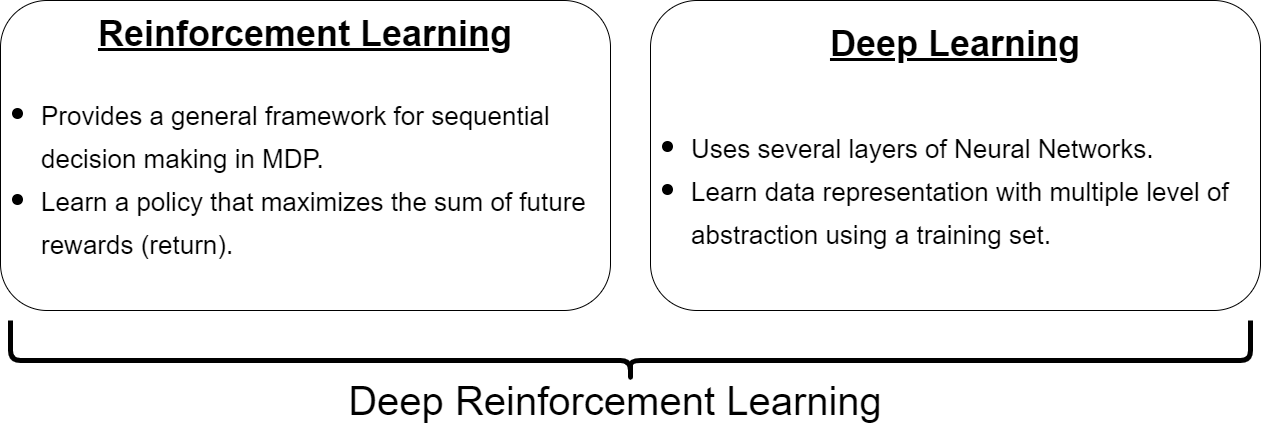
\includegraphics[width=\textwidth]{Figures/Ch_RL/RL_intro_DL_RL2.png}
    \caption{RL and DL combine to form DRL paradigm of algorithms.}
    \label{fig:RL_DL_RL}
\end{figure}

\begin{figure}[h!]
    \centering
    \includegraphics[width=\textwidth]{Figures/Ch_RL/RL_intro.png}
    \caption{Application of DRL in the field of (a) Atari games, (b) Game of Go and (c) Robotics}
    \label{fig:RL_intro}
\end{figure}

DRL is expected to revolutionize the field of AI and represents a step towards building autonomous systems with a higher-level understanding of the physical world. The field received a lot of attention for the development of an algorithm that can play a range of Atari games \parencite{silver2016mastering}. This was a breakthrough in artificial intelligence since scientists thought that it would take many more years to make machines win such complex games. Currently, deep NNs are enabling reinforcement learning to scale to previously intractable problems, such as creating a single system that can play multiple video games directly from pixels, named AlphaGo \parencite{silver2016mastering} and AlphaGo Zero \parencite{silver2017mastering}. DRL algorithms are also applied to robotics \parencite{kober2013reinforcement}, allowing control policies for robots to be learned directly from sensory inputs in the real world \parencite{levine2016end}, designing algorithms to automatically learn to allocate and schedule computer resources to waiting jobs, with the objective to minimize the average job slowdown \parencite{mao2016resource}, design a traffic light controller to solve the congestion problem \parencite{arel2010reinforcement}, Bidding and Advertisements \parencite{jin2018real}. Recently, DRL was tested on predicting the 3D shape that a protein will fold into. The results of the biennial protein-structure prediction challenge called CASP (Critical Assessment of Structure Prediction) is seen as a breakthrough in the application of DRL in the field of drug discovery \parencite{senior2020improved}, which is seen as a field that is not part of the conventional RL domains. While the present achievements of DRL in the field of robotics and computer games are impressive and required a massive amount of resources to discover, this chapter extends the work in the field of DRL to Topology Optimization.

\section{Literature survey}

\subsection{Application of ML algorithms in TO}

In the past decade, machine learning algorithms have been extensively studied in the field of Topology Optimization. This is due to the capability of ML algorithms to approximate highly non-linear functions. A trained ML surrogate model is capable of predicting structures based on the patterns and behaviors learned from the analysis of several examples. Machine Learning (ML) and in particular Deep Learning (DL) have also demonstrated some capabilities in reducing the computational cost associated with topology optimization. A comparison for most of the recent work in the field of TO involving ML algorithms is shown in Table \ref{tab:lit_rl}. As can be seen, most of the work is based on labeled data and involves supervised learning algorithms. After training with optimized solutions from conventional methods for TO- gradient-based or stochastic methods, a neural network can be trained in a supervised manner to predict solutions of the same TO problem under different input conditions. The differing conditions represent the geometries obtained during the process of TO optimization. In the field of solid mechanics, \cite{yu2019deep} used 100,000 optimal solutions to a simple mechanical compliance problem (distributing material in a domain so that the structure achieves maximum stiffness for given loading and constraints) with various boundary forces and the optimal mass fractions to train a neural network consisting of a Convolutional Neural Network (CNN) \parencite{lecun1998gradient} and conditional Generative Adversarial Network (cGAN \parencite{goodfellow2014generative}), which can predict near-optimal designs of mass fraction for any given boundary forces. Further, \cite{chandrasekhartounn} used neural networks to represent the density parameter in the Solid, Isotropic Microstructures with Penalization (SIMP) approach \parencite{rozvany1992generalized} for a TO process. In another approach, \cite{banga20183d} showed the potential of a 3D Encoder-Decoder based approach to convert the TO problem to an image segmentation \parencite{badrinarayanan2017segnet} one. The first usage of DL algorithms in the field of TO \parencite{sosnovik2019neural} in recent years was to use a Deep CNN Autoencoder to reduce input dimensionality. The latent information (usually extracted from the center-most hidden layer) extracted from a trained CNN-based Autoencoder helped in cutting down the computational time through dimensionality reduction but was not used as an optimization algorithm for TO. 

It should be noted that all the researches listed above belong to supervised learning, which is a class of ML algorithms based on static and pre-computed training data, where the input-output (features-labels) pair must be provided. Thus, they suffer from a lack of generalizability and have been criticized in \cite{deng2020deep} as not a TO algorithm, since they rely on existing optimal designs as the training data. The predictions are restricted by the coverage of the training dataset and thus are biased on the methodology for collecting the training samples. This can introduce data collection bias to the model, as a surrogate DL model will provide highly accurate results to the design space part of its training data. For any unseen new geometry, the performance of the ML model will be unreliable, if not inaccurate. To consider different domain geometries, these approaches will require new datasets and train new neural networks for any change in the conditions of the TO problem. This issue has been the focus of recent works. \parencite{zhang2019deep} used a DL method based on CNN and GANs for TO with generalizability ability where instead of mapping sparse boundary conditions, physical fields were found to allow the Neural Network (NN) to learn a more accurate mapping between the boundary condition and the optimal structure. Thus, the advantage proposed by \cite{zhang2019deep} comes from the well-designed input form, enabling the DL model to solve TO problems with different boundary conditions even though the training datasets had only one or a few boundary conditions. Nonetheless, the learning methodology used in \cite{zhang2019deep} is supervised and has the same shortcomings as mentioned previously. Smart input encoding does not solve the underlying problem associated with supervised learning methodologies.
% Please add the following required packages to your document preamble:
% \usepackage{graphicx}
\begin{table}[h!]
\centering
\resizebox{\textwidth}{!}{%
\begin{tabular}{|c|c|c|c|c|c|}
\hline
\textbf{Paper}                             
& \textbf{\begin{tabular}[c]{@{}c@{}}Learning \\ Architecture\end{tabular}} 
& \textbf{\begin{tabular}[c]{@{}c@{}}Online \\ Learning\end{tabular}}
& \textbf{\begin{tabular}[c]{@{}c@{}}Design \\ Optimizer\end{tabular}} 
& \textbf{\begin{tabular}[c]{@{}c@{}}Generaliz- \\ abile\end{tabular}}
& \textbf{\begin{tabular}[c]{@{}c@{}}Manufactur-\\ alibility \\ (part of TO)\end{tabular}} 
\\ \hline \hline
\parencite{chandrasekhartounn}     & Feedforward     & \xmark   & \xmark     & \xmark                               & \xmark                    \\ \hline 
\parencite{banga20183d}            & CNN             & \xmark   & \textcolor{green}{\cmark}     & \xmark          & \xmark   \\ \hline
\parencite{sosnovik2019neural}     & CNN             & \xmark   & \xmark   & \xmark                                & \xmark                      \\ \hline
\parencite{lei2019machine}         & KNN, SVM        & \xmark   & \textcolor{green}{\cmark}     & \xmark          & \xmark     \\ \hline
\parencite{nie2020topologygan}     & GANs            & \xmark    & \textcolor{green}{\cmark}     & \xmark          & \xmark     \\ \hline
\parencite{yu2019deep}             & CNN + cGAN      & \xmark    & \xmark  & \xmark                                & \xmark                        \\ \hline
\parencite{deng2020deep}           & Feedforward     & \textcolor{green}{\cmark}    & \xmark  & \textcolor{green}{\cmark}             & \xmark       \\ \hline
\parencite{doi2019multi}           & CNN             & \textcolor{green}{\cmark}   & \xmark  & \xmark              & \xmark  \\ \hline
\parencite{sasaki2019topology}     & CNN             & \xmark    & \xmark  & \textcolor{green}{\cmark}     & \xmark                          \\ \hline
\parencite{barmada2020deep}        & CNN             & \xmark    & \xmark  & \textcolor{green}{\cmark}     & \xmark                           \\ \hline
\end{tabular}%
}
\caption{Literature survey of ML papers in Topology Optimization}
\label{tab:lit_rl}
\end{table}

\begin{comment}
\parencite{ulu2016data}         &                                                                           &                          &                    &                           & No                                                                                         \\ \hline
\parencite{lin2018investigation}                       &                                                                           &                          &                    &                           & No                                                                                         \\ \hline
\parencite{zhang2019deep}          &                                                                           &                          &                    &                           &                                                                                            \\ \hline
\end{comment}

Furthermore, another issue associated with supervised learning is that the material (volume) constraint is treated as a condition to match as closely as possible rather than a true inequality constraint. This is due to the nature of supervised learning where the optimization algorithm tries to minimize a loss function to as low a value as possible. Due to the above-mentioned problems with supervised learning, \cite{deng2020deep} limited the use of ML algorithms as a performance estimator (rather than an optimization algorithm) for the compliance minimization problem in mechanics. \cite{deng2020deep} trained the DNN in an online fashion, where the training data was selectively collected to capture near-optimal solutions. Although this helped in accelerating the computation by using a DNN as a surrogate of the objective function evaluator, the ML algorithm is not involved in the TO process and thus does not influence the generation of new topologies. Further, as this approach limits the data generation for training only on near-optimal solutions, it will obstruct the ability of the network to distinguish between a good and a bad solution. As a consequence of a network trained with a highly imbalanced dataset, it can overestimate the performance indicator for a poor design and will affect the performance of the stochastic algorithm itself.

\subsubsection{Advancements in TO for Electromagnetics}
In the field of electromagnetics, \cite{sasaki2019topology} introduced TO for EM analysis where a CNN-based performance estimator is used to predict the torque values for the optimization of IPM motors. Further advancements were performed in \cite{doi2019multi} and \cite{barmada2020deep} where incremental efforts were made to reduce the computation burden associated with FE analysis. These approaches used DL methods as a filter for removing the inferior population at any iteration of the GA process. The best-performing designs are reevaluated with FEA to reduce the computation burden. This type of supervised learning has been implemented in both an on-line \parencite{doi2019multi} and off-line fashion \parencite{sasaki2019topology}. 

\subsection{Addressing the Disadvantages of Supervised Learning in TO}

Given the advantages associated with involving ML algorithms, there is a motivation to extend the above-mentioned works by pursuing a methodology that focuses on extending generalizability as a part of the optimization process rather than using DL as a surrogate or labeled data-constrained supervised learning for TO. For this purpose, the concept of DRL is introduced for TO in this Chapter. 
In addition, the concept of manufacturability from Chapter \ref{chapter:4_MDP} is also an important criterion and should be included from the initial phase of TO with RL.

\begin{comment}
\subsection{Technology - GD}
Too Many Choices
While this may seem counterintuitive, having a wide variety of choices is not always desirable. An unreasonably large number of choices can easily overwhelm the architect and in some cases, actually require more time to handle than creating a manual design from scratch.

This problem, though, gets better over time as the program learns how to sort the options, using previously data about the final solution selection.

Generative design technology is a culmination of the awesome power of AI, ML, and a designer’s talent. With the advent of high processing power and advanced scripting capabilities, this technology is surpassing its original constraints to give us amazing designs.

The generated products are capable of following every specified requirement and constraint to provide us with truly innovative CAD models perfect for our needs.
Today, there are still only a few industries that can actually benefit by lowering their overall costs. For example, Airbus shaved off 45\% (30 kg) off the weight of a single part. The fuel consumption decrease equalled to removing 96,000 cars off the road for a year.

Machine learning features enable the software to learn from experience and the design quality improves with time.
Generative design can be used to reduce weight in places previously neglected to achieve innovative lightweighting. This is an important reason generative design has been adopted eagerly in the aerospace and automobile industries.
\subsection{Issues with Generative Design}
While traditional methods such as topology optimisation can also reduce cost overruns and waste, they only provide us with one solution.

Generative design, on the other hand, provides us with a long list of possible models all of which would be within our specified budget with minimal wastage.

Through additive manufacturing processes, these parts with complex geometry can be manufactured with ease. This ultimately reduces the number of parts in the assembly.

It also simplifies the supply chain and maintenance while reducing the cost of production.

\end{comment}

\section{Setting up Deep RL}

The usage of deep reinforcement learning aims to create a system that can adapt to novel geometries through the use of suitable system dynamics in the form of an MDP and the usage of neural networks as function approximators, which can generalize to new geometries and excitations. This section contains a discussion on the setup of function approximator following a modification of Q-learning from Tabular (Section \ref{subsubsec:MDP_Q_learning}) to Deep Q-Learning methodology, along with the changes introduced in the MDP, in comparison to the one discussed in Section \ref{section:MDP_MDP}. As with Chapter \ref{chapter:4_MDP}, the term `FE calls' is used to refer to the number of simulations performed in a corresponding optimization task. Although a FE solver is used for all electromagnetic analyses in this study, this is 
neither a necessary requirement nor a limitation associated with any of the optimization algorithm discussed in this work. Any EM solver to be used, as long as it is able to provide an accurate solution and a performance measure required for the operation of the algorithm, such as force magnitude and field distribution.

\subsection{Advanced Function Approximators}

This section builds on the Tabular QL algorithm discussed in Chapter \ref{chapter:4_MDP} Section \ref{subsubsec:MDP_Q_learning}, where a greedy policy was obtained for optimal material placement. This involved learning the value function (Q-value) for the states and action pair associated with a TO environment (SeqTo-$v1$). The tabular QL approach will not be able to expand to high dimensional state and action space, due to the curse of dimensionality. It is not possible to compute and preserve the  value function (Q-value) for all possible state-action pairs, especially when either of them (state or action) is continuous. Further, a more complex action space adds to the curse of dimensionality problem, making the tabular method either infeasible or too memory intensive. There are other ways to store and represent a value function. This chapter introduces function approximation to approximate the action values. These function approximators can be expressed with a relatively small number of parameters.  The ML literature consists of many ways to parametrize an approximate value function (Q or V) such as Linear Regressors, Decision Trees, SVMs, and Neural Networks to name a few classes of available options. In principle, any function that takes the state as an input and produces a (or a set of) real number(s) that represents the value associated with that state, is considered suitable enough to be used as a function approximator for value function (Q or V). A popular category used for this is parametrized functions where a set of real-valued weights are adjusted to learn a representation from the state space to the corresponding action value. These weights can be tuned to allow for a change in the output of the parameterized function to account for collected experience as and when the experience is generated in a sequential learning format. The aim is to generate an Action value function predictor $\hat{Q}(s,a, w)$ which approximates the true action-value function $Q_{\pi}(s,a, w)$. This is better than the tabular approach (Chapter \ref{chapter:4_MDP}), for large state and action spaces. 
Further, the tabular approach worked only with an integer-based encoding of the design domain, as shown in Figure \ref{fig:RL_state_repr_original}. For a richer encoding technique as shown in either Figure \ref{fig:RL_state_repr_2} or \ref{fig:RL_state_repr_3_Bfield}, the tabular approach is not an appropriate form of storage. The floating-point data type needed to represent the magnetic field distribution in the air gap (Figure \ref{fig:RL_state_repr_2}) and the whole geometry (Figure \ref{fig:RL_state_repr_3_Bfield}), will be either infeasible or will require high memory capacity, as mentioned earlier. Alternatively, an attempt to discretize the continuous magnetic field values will result in a precision trade-off. In such cases (Figure \ref{fig:RL_state_repr_2} \& \ref{fig:RL_state_repr_3_Bfield}), a parametrized approximator is ideal for representing a state of the design domain which includes the magnetic field distribution and offers the flexibility of dealing with similar problems including geometries and excitation. Thus taking the advantage of parameter fitting and interpolation.

\begin{align*}
    \hat{v}(s, w) \approx v_{\pi} (s)
\end{align*}

Another difference between the tabular and parameter-based methodology is that modifying a single entity of the value function table leaves the value functions associated with other states (s) or state-action pair (s, a) unchanged. Now the learning algorithm will modify the weights of a parametrized function and will affect states which are closely related in the weights distribution space. For parametric representation, the learning algorithm will modify the weights of the parametrized function and this change will affect all the values associated with other states (s) or state-actions(s, a) that are closely related to the weight distribution space. 

\begin{table}[h!]
\centering
\begin{tabular}{|c||c|c|c|c|}
\hline 
      & $a_0$ & $a_1$ & $a_2$ & $a_3$ \\ \hline \hline
\textbf{$S_0$} & \circled{\textcolor{red}{8.2}}   & -0.2  & 4.1   &  4.4 \\ \hline
\textbf{$S_1$} & \circled{\textcolor{red}{6.6}}   & -1.0  & -1.5  &  5.6 \\ \hline
\textbf{$S_2$} & -3.3  & -2.6  & \circled{\textcolor{red}{11.1}}  & -4.7  \\ \hline
\end{tabular}
\caption{Example of a Q-table}
\label{tab:RL_Q_table}
\end{table}

The simplest form of function approximator is a linear function, which is a linear representation of the constituent weights for the Q-value (Table \ref{tab:RL_Q_table}). These weights are multiplied with the features to get a scalar value for a state Action-value function. The features are some fixed attributes that explain the state. The performance of linear function approximators relies on good features that are capable of discriminating between different state-action pairs.
Tabular representation is a special case of linear function approximation, where each state-action pair is a separate feature and thus requires a weight/Q-value for each instance of the state-action pair. This can be stated in the following equation as :

\begin{align*}
    \hat{Q} (s_i,a_j, w) & \doteq <w,x(s_i, a_j)>\\
                     & =  w_{ij}
\end{align*}
where $x(s_i, a_j)$ is one-hot encoding \parencite{geron2019hands}. One-hot encoding is used since only a single entry in the Q-table will correspond to a state-action pair ($s,a$), as can be seen from the Table \ref{tab:RL_Q_table}. One-hot encoding will produce a vector with only a single non-zero element (high) which corresponds to the highest possible value for each row of the Q-table.

So a tabular representation is the same as a linear approximation with the number of weights the same as the number of states, which, as stated above, is suitable for a small integer encoded state-action space. Neural networks, on the other hand, implement a non-linear function of the states. The state, or features representing the state, is passed to the neural network as an input. All the connections through hidden layers correspond to real-valued weights. When data is passed through a connection the weight gets multiplied by the input. The weights form a connection between any two layers in the neural network.
The process transforms the input state through a sequence of layers to finally produce the action value estimate as to the output of the neural network, as shown in Figure \ref{fig:RL_nn_architecture}. The field of Deep Reinforcement Learning (Deep RL) deals with using Neural networks in combination with the learning algorithms of RL such as (Q-learning, Monte Carlo, Policy Gradients).

\begin{figure}[h!]
    \centering
    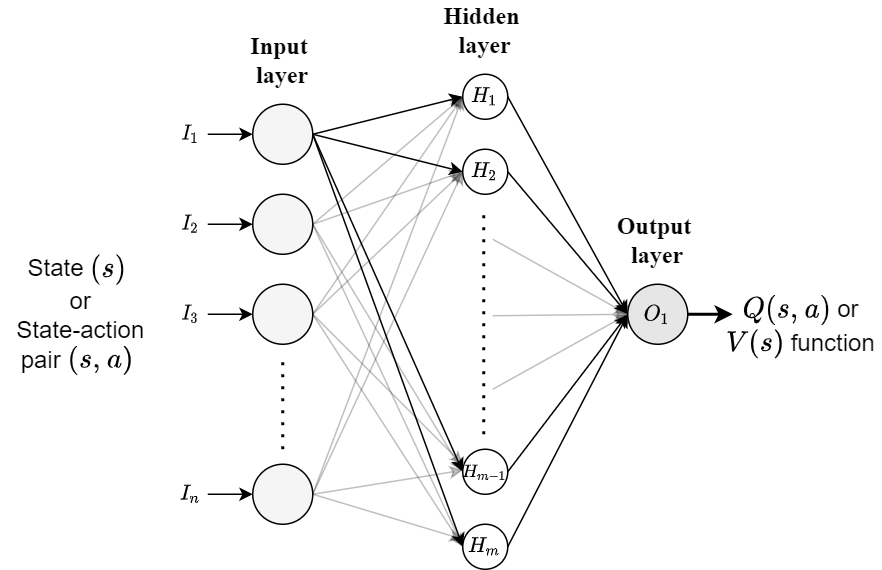
\includegraphics[width=0.6\textwidth]{Figures/Ch_RL/RL_nn_architecture_2.png}
    \caption{Feedforward neural network for Value function ($Q(s,a)$ or $V(s)$).}
    \label{fig:RL_nn_architecture}
\end{figure}

Although there are other possibilities for a function approximator, there are criteria that must be satisfied to produce a satisfactory predictor for the value function. It should possess the property of both generalizability and discrimination. Generalizability is the ability to apply knowledge about a specific scenario to a variety of similar situations. An update to the value estimate of one state-action pair influences the value estimate of other statistically similar state-action pairs. This is also helpful in speeding up the learning by making better use of the experience generated and ultimately help in faster convergence to the optimal solution (design), as not all distinct state-action pairs need to be visited. 
On the other hand `Discrimination' is an ability to distinguish two significantly different states, by assigning different values in the form of prediction to significantly different states. There might be some states with similar features (as they have similar geometry) but drastically different returns. An example of this can be seen in Figure \ref{fig:RL_c_core_negative_error}. An ideal candidate for a function approximator should be able to find distinguishable features that can help with the separation. Tabular methods are great at distinguishing two states perfectly but do not generalize at all. Each state-action pair is represented by a distinct entry in the table (Table \ref{tab:RL_Q_table}). Each entry of the state-action pair ($s, a$) is independent of each other. Thus, the controller is forced to visit all the state-action pairs in the MDP to be able to find a greedy policy. A neural network on the other hand is good at finding a balance to the generalizability-differentiability trade-off \parencite{hornik1989multilayer}, conditioned that the features representing the states contain sufficient information. For the scenario shown in Figure \ref{fig:RL_c_core_negative_error}, additional information along with the material distribution such as magnetic field distribution can help the function approximator with balancing the trade-off.

\begin{figure}[h!]
    \centering
    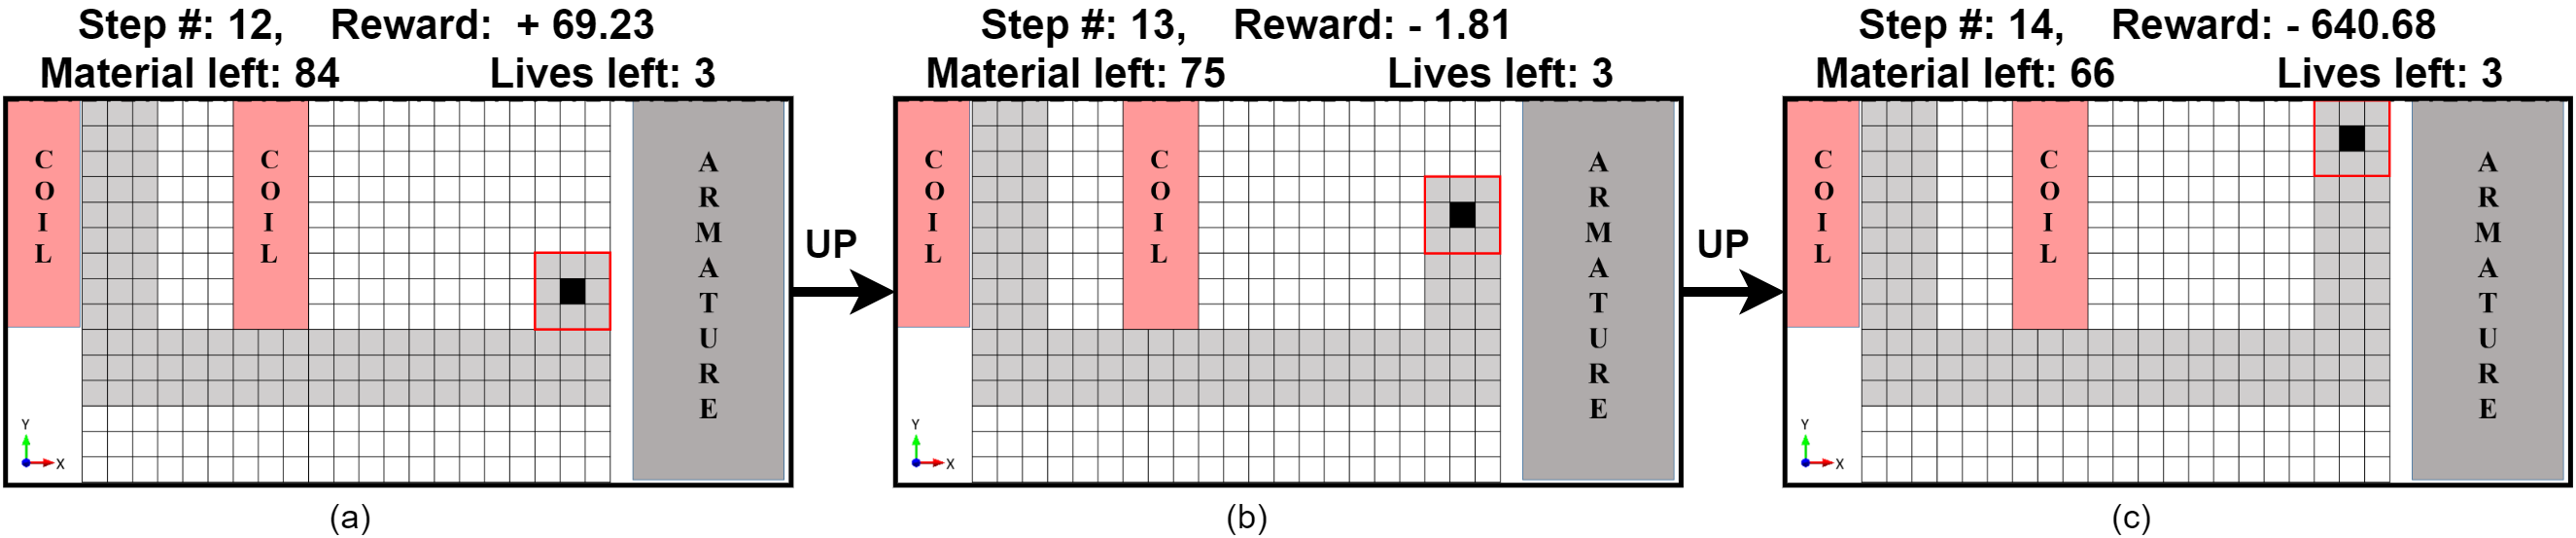
\includegraphics[width=\textwidth]{Figures/Ch_RL/c_core_negative_error2.png}
    \caption{Sudden decrease in performance with a slight change in the state representation. Coil Current: 1.5 Amps, No. of Turns: 500.}
    \label{fig:RL_c_core_negative_error}
\end{figure}

An additional characteristic that the learning system should have is the ability to learn in a sequential manner. This is in contrast to supervised learning as the data generation process in an RL task is online. The online nature of the data is attributed to the constant interaction of the agent with the environment. On the other hand, the data used in supervised learning is pre-generated and is independent of the current weights of the neural network. This dynamic interaction makes the data generated at any given time dependant on how well the agent understands the environment. This creates a non-stationary distribution of the training data, where previous knowledge gained by the learning system is to be discounted in favor of the new experience. This is one of the reasons why sample efficient algorithms are an active area of research in the field of Deep RL \parencite{henderson2018deep}. On top of that the ever-present challenge of reducing the computation cost associated with the task of TO. Identifying an ideal learning system that balances all the above-mentioned requirements is a difficult job and is heavily task-dependent. A learning system based on non-linear function approximators such as Neural networks is ideal for generalization, discrimination, and online learning but will require significantly more training examples to train as compared to a tabular method. However, the cost of higher sample requirements can be justified with the ability to generalize over similar optimization tasks.

\subsection{Objective of the RL Task}
\label{section:RL_Objective_of_the_RL_Task}
The value estimation problem can be setup as a supervised learning task. The first task is to define an objective to optimize. A regression task can be setup such that the error is stated as:
\begin{align}
    \text{Error (MSE) } = \Big[Q^*(s, a) - \hat{Q}(s, a, w)\Big]^2 \label{eqn:RL_Obj-MSE}
\end{align}

Although the problem is formulated in the sense of supervised learning, it will be difficult to match the true value ($Q^*(s, a)$) of the action-value function at all states. Also, in most problems, the optimal value function ($Q^*(s, a)$) is unknown at the beginning of the training. 
Unlike the supervised learning tasks (e.g. the Field \& Performance maps estimation), a high accuracy value that has been obtained in Chapter \ref{chapter:2_CNN} \& \ref{chapter:3_RNN} does not necessarily reflect in a value function being a good predictor for the true action-value function. In the absence of the optimal value function ($Q^*(s, a)$), (as was discussed in Chapter \ref{chapter:4_MDP}, Section \ref{section:MDP_QL-Value_Function}, in Temporal Difference (TD) learning), the learning algorithm uses it's own estimate of the value function to update it's own prediction. Another alternative is to use an estimate of the return ($G_t$), but as was discussed in Chapter \ref{chapter:4_MDP}, Section \ref{subsubsec:MDP_Q_learning}, the computation cost associated is too expensive.

For making an update to decrease the error on an experience trajectory:
\begin{align}
(S_1, A_1), Q_{\pi}(S_1, A_1) \rightarrow (S_2, A_2), Q_{\pi}(S_2, A_2) \rightarrow (S_3, A_3), Q_{\pi}(S_3, A_3) \rightarrow \hdots
\end{align}

will be determined by the gradient of the loss function from Eq. \ref{eqn:RL_Obj-MSE}:
\begin{align}
    \alpha \nabla \Big[Q_{\pi}(s, a) - \hat{Q}(s, a, w)\Big]^2
\end{align}

Using the estimation of the return as an approximation for the true Value function, for making updates in the weights ($w$) of the neural network predicting the action value function ($Q(s,a)$:

\begin{align*}
    w \longleftarrow w + \alpha [G_t - \hat{Q}(s_t,a_t w)]\nabla \hat{Q}(s_t, a_T, w)
\end{align*}

This updates the weights ($w$) of the neural network such that the action value estimate is closer to the return ($G_t$) of the sample experience trajectory. The return can be replaced with any other estimate of the action-value function. Similar to Section \ref{subsubsec:MDP_Q_learning}, instead of the return ($G_t$), a bootstrap target based on the action-value of the next step resulting in the following error equation:

\begin{align}
    \text{Error (MSE) } = \Big[R_t + \max_{a'}\hat{Q}(S_{t+1}, A_{t+1},w) - \hat{Q}(S_t, A_t, w)\Big]^2
\end{align}

\begin{figure}[h!]
    \centering
    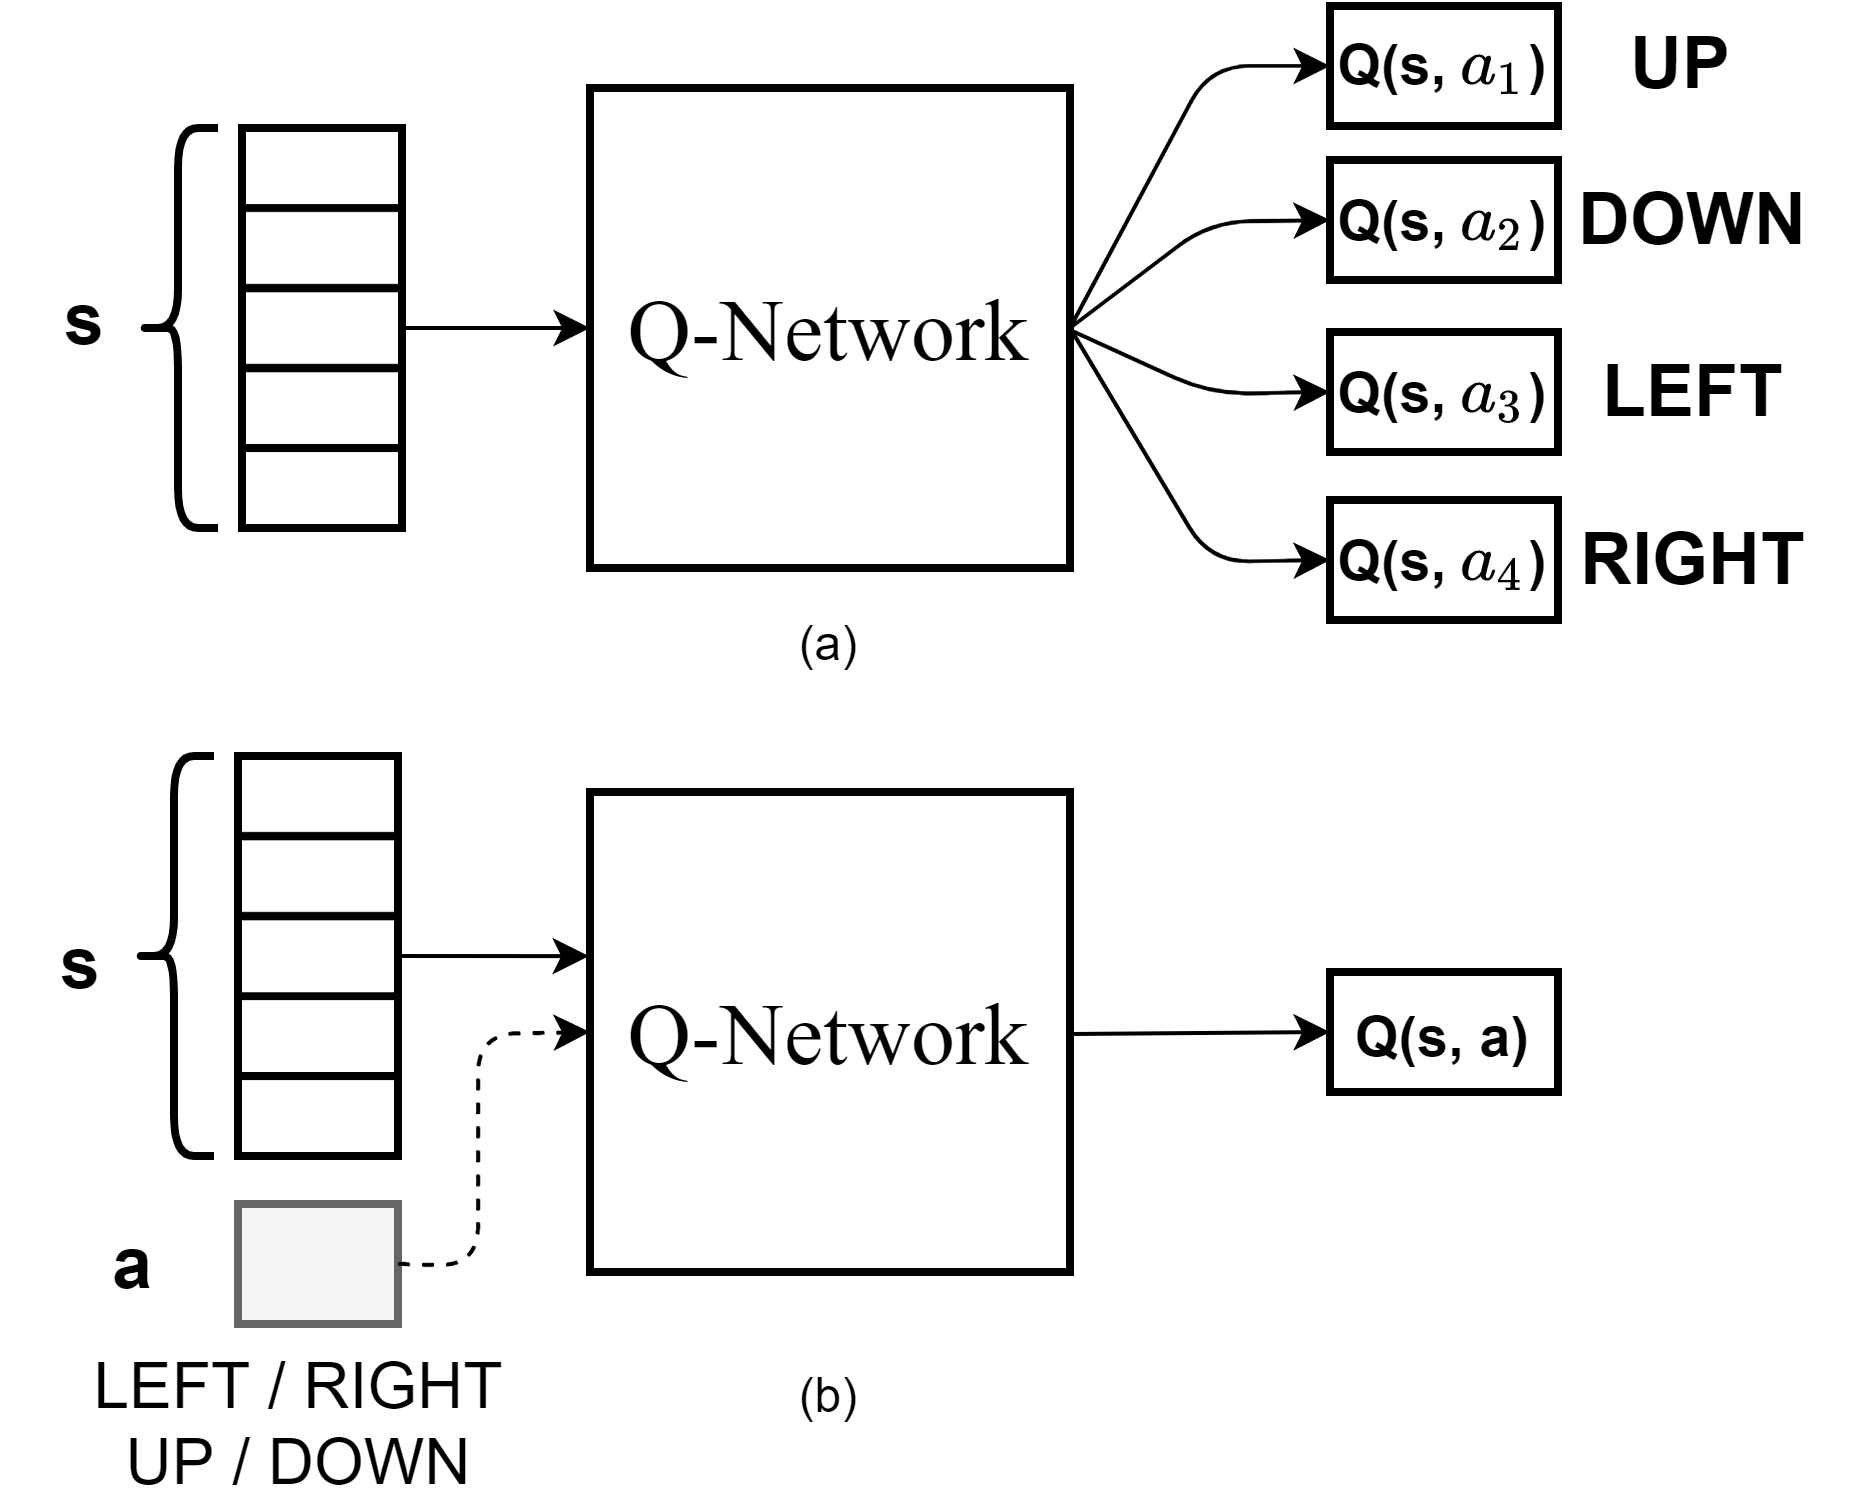
\includegraphics[width=0.75\textwidth]{Figures/Ch_RL/QL.png}
    \caption{Different approaches of setting up the Q-Network}
    \label{fig:RL_QL_network_types}
\end{figure}

The Q-learning with neural networks is implemented by stacking the actions in one neural network, such that a single network predicts the action value associated with all possible actions in the state as shown in Figure \ref{fig:RL_QL_network_types}.
The weights in the Q-learning neural network are updated as follows:
\begin{align}
    w \longleftarrow w + \alpha [R_{t+1} + \hat{Q}(s_{t+1},a_{t+1}, w) - \hat{Q}(s_t,a_t, w)]\nabla \hat{Q}(s_t, a_t, w)
\end{align}

This method of learning is called on-policy learning. A more complex version of it, uses two neural networks for learning the $Q(s,a)$ value. One is called the behaviour Q-Network and the other is target Q-network, resulting in the following update equation:

\begin{align}
    w \longleftarrow w + \alpha [R_{t+1} + \hat{Q}_{tar}(s_t,a_t, w_{tar}) - \hat{Q}_{beh}(s_t,a_t, w_{beh})]\nabla \hat{Q_{beh}}(s_t, a_T, w_{beh}) \label{eqn:RL_behaviour_target_policy}
\end{align}

where $\hat{Q}_{tar}(s_t,a_t, w_{tar})$ is the target policy and $\hat{Q}_{beh}(s_t,a_t, w_{beh})$ is the behaviour policy. The behaviour NN is responsible for suggesting actions while collecting the experience. The target policy on the other hand does not interact with the environment directly but is used to train the behaviour policy using the eqn. \ref{eqn:RL_behaviour_target_policy}. The target policy is obtained from the behaviour policy by the timely transfer of weights from the behaviour policy (shown as `Knowledge Transfer' in Figure\ref{fig:RL_Q_learning_cycle}). This method of learning is called off-policy learning, as the policies used for generating experience and training are different. This type of learning has shown improved performance in the training of Q-learning \parencite{hasselt2010double}.

$\epsilon-$greedy is used for exploration for both off-policy and on-policy, same as that in Section \ref{section:MDP_QL-Value_Function}, where the emphasis is on exploration of the environment at the start of the training and as the agent learns the dynamics of the environment the scale of exploration is gradually decreased.

\begin{align}
    a_t  = 
    \begin{cases}
        \underset{a}{\arg\max} \; Q_{(beh)}(s, a; w_{(beh)}) \quad & \text{with probability} \; 1- \epsilon \\
        a \sim \uniform (a_1, \hdots a_k) \quad & \text{with probability} \; \epsilon
    \end{cases}
\end{align}

Finally, it is also not expected that the approximator is giving great performance on all possible state-action pairs. Importance should be given to samples (state, action) from experience which the policy visits more often than others. Samples that occur more compared to others in a policy should be weighted higher than the ones where the time spent is less.  

An agent needs to try many different actions in numerous states to try and learn all the available possibilities and to find the optimal material distribution which will maximize its overall reward; this is known as `Exploration', as the agent is searching for better prospects in the environment. On the other hand, if all the agent will do is random exploration, it will never maximize the overall reward so it must also use the information it learned from the experience. This is known as `Exploitation', as the agent exploits its knowledge to maximize the rewards it can receive.
The trade-off between the two is one of the most significant challenges of RL problems, as the two must be balanced to allow the agent to both explore the environment enough, but also exploit what it has learned and repeat the most rewarding path it found.

\begin{figure}[h!]
    \centering
    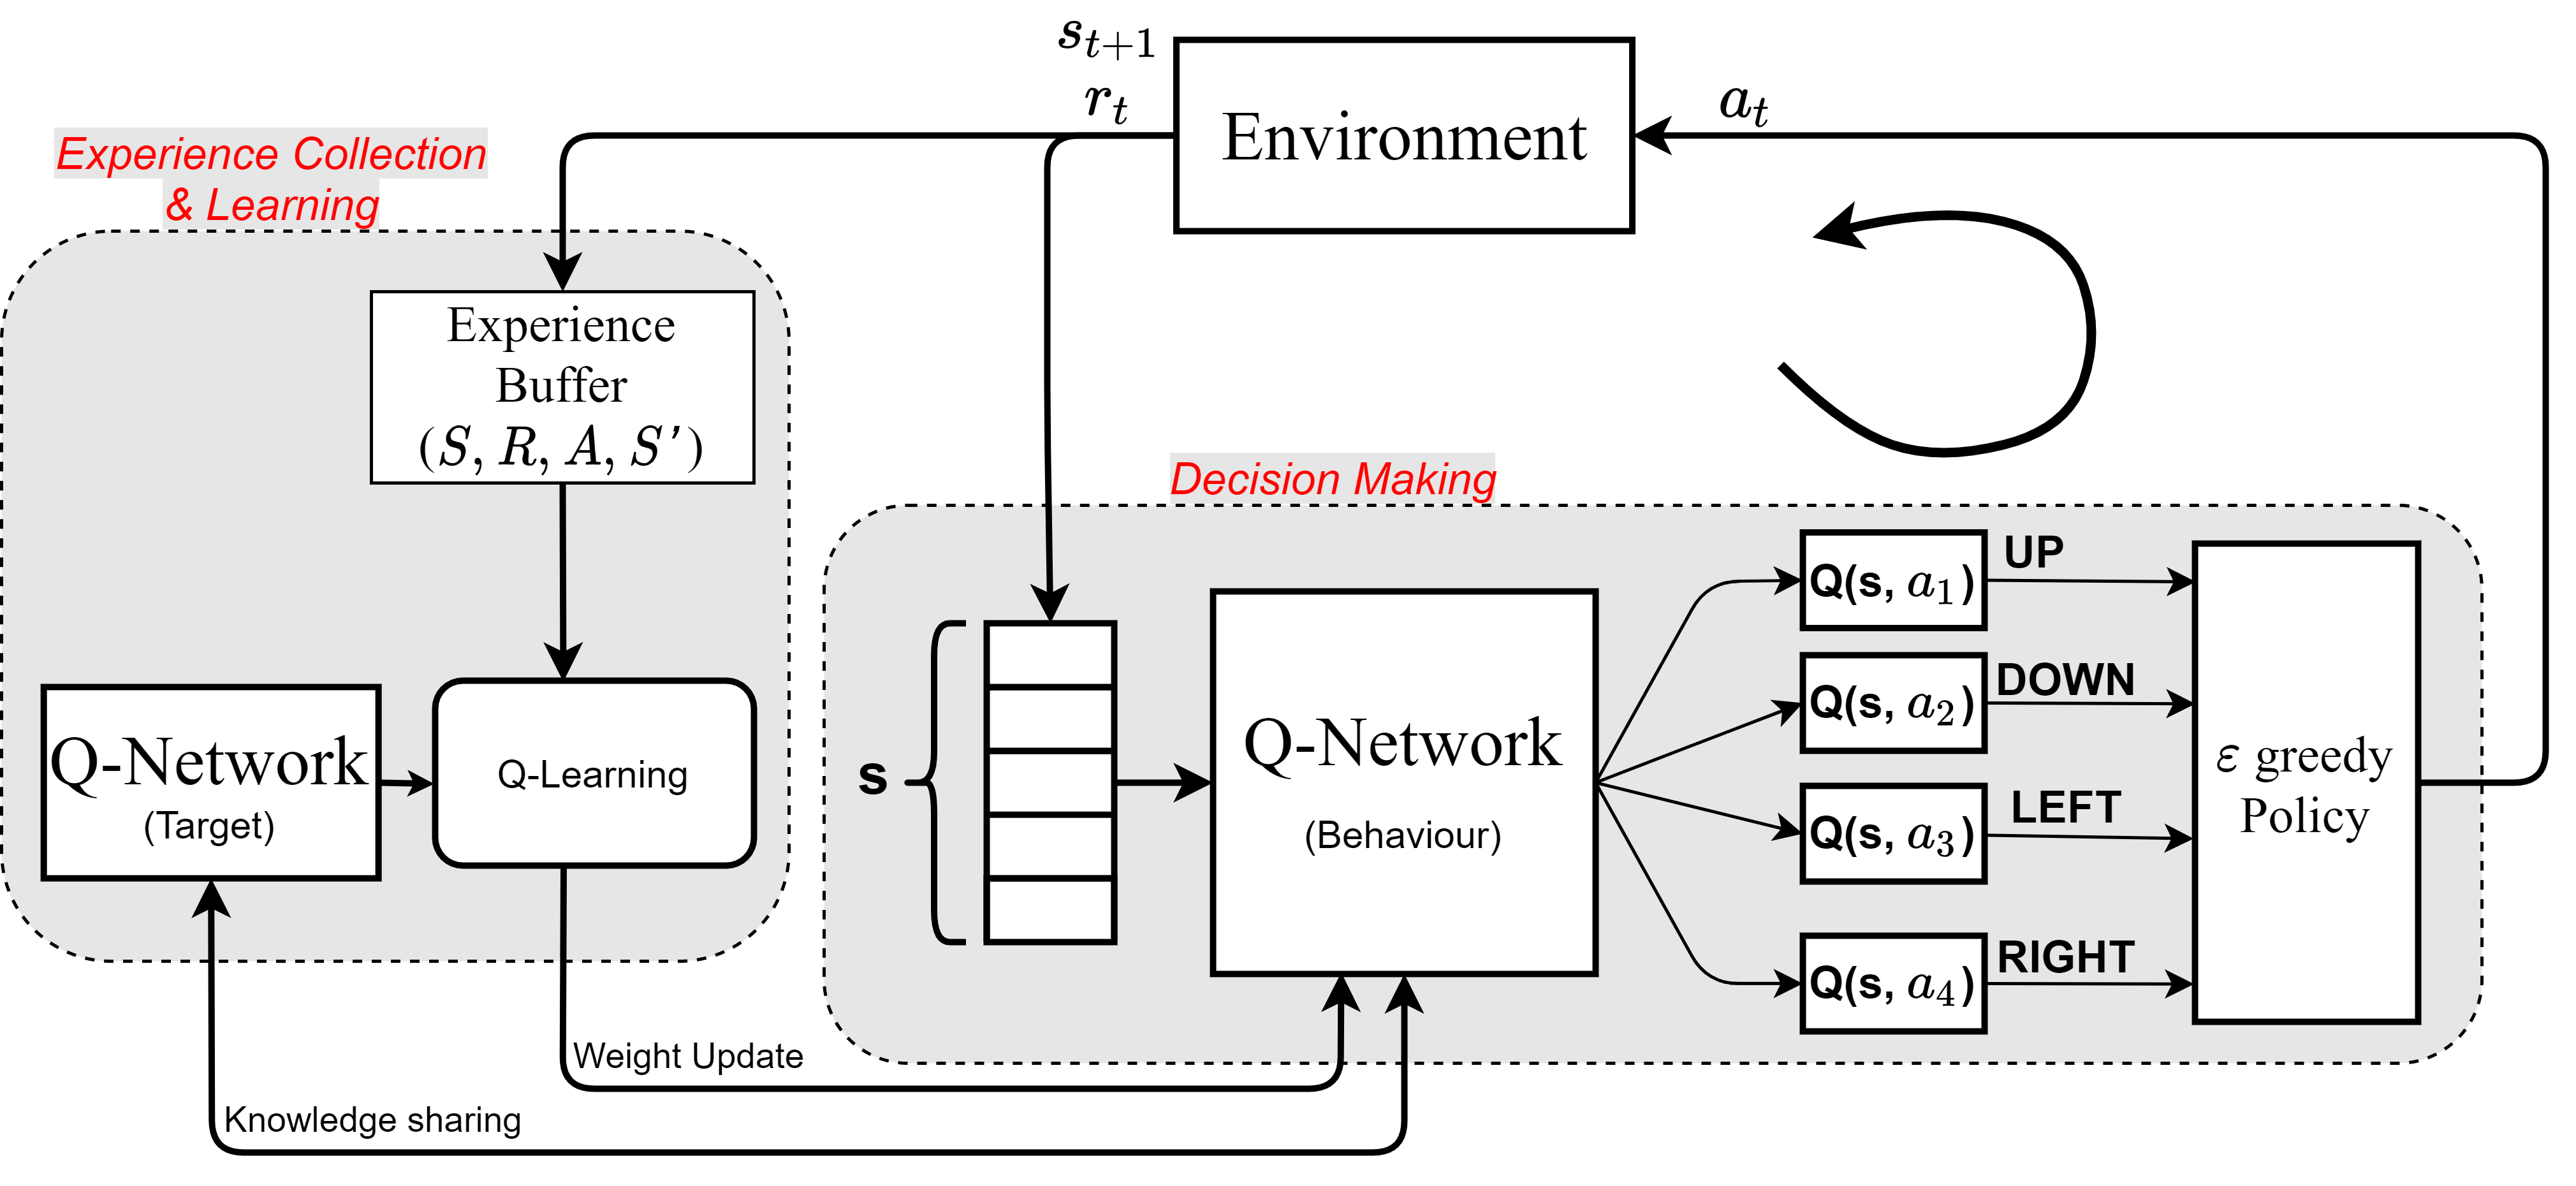
\includegraphics[width=0.95\textwidth]{Figures/Ch_RL/QL_full_in_depth.png}
    \caption{Q-Learning Cycle}
    \label{fig:RL_Q_learning_cycle}
\end{figure}

\subsection{Experience Replay}
\label{section:RL_Experience_Replay}

As RL tasks have no pre-generated training sets which they can learn from, the agent must keep records of the state transitions it encountered so that it can learn from them later. The memory buffer used to store this is referred to as `Experience Replay'. There are several types and architectures of these memory buffers - but some very common ones are the cyclic memory buffers, which make sure the agent keeps training over its new behaviour rather than transaction experience that might no longer be relevant. The memory operation of a cyclic memory buffer behaves like that of a queue, where the oldest entry is removed first, once the buffer reaches its capacity. Another type of memory buffer is reservoir-sampling-based, which guarantees each state-transition recorded has an even probability to be inserted into the buffer. In this work, only cyclic memory buffers were used since they limit the amount of memory required for storing the experience buffer.

\subsection{Deep Q-learning}

DeepMind's DQN (Deep Q Network) was a breakthrough success in applying deep learning to RL problems \parencite{mnih2013playing}. Combining the previously discussed concepts of Experience Replay, $\epsilon$ based exploration, and the algorithm of Q-learning the algorithm is used to train a Neural Network (Q-Network, referred as DQN) to find an optimal policy that is greedy on the cumulated reward function. Algorithmically, DQN is related to the tabular Q-learning algorithm discussed in Section \ref{subsubsec:MDP_Q_learning}. However, the key difference is the involvement of advanced functional approximators for replacing state-action table (from Q-learning; Section \ref{subsubsec:MDP_Q_learning}) with a neural network to cope with large-scale tasks, where the number of possible state-action pairs can be enormous. This variation introduces two key addition to the Q-learning procedure: Experience Replay (discussed in Section \ref{section:RL_Objective_of_the_RL_Task}) and the use of a separate target network (Section \ref{section:RL_Objective_of_the_RL_Task}). The setup of the function approximation-based Q-learning method is shown in Figure \ref{fig:RL_Q_learning_cycle}. The core of the C-core (shown in Figure \ref{fig:RL_c_core_conventional_design_domain}) is to be designed using TO such that the force experienced by the armature is maximized. The excitation for the current coil is set at 1.0 Amps with 500 turns.

\begin{figure}[h!]
    \centering
    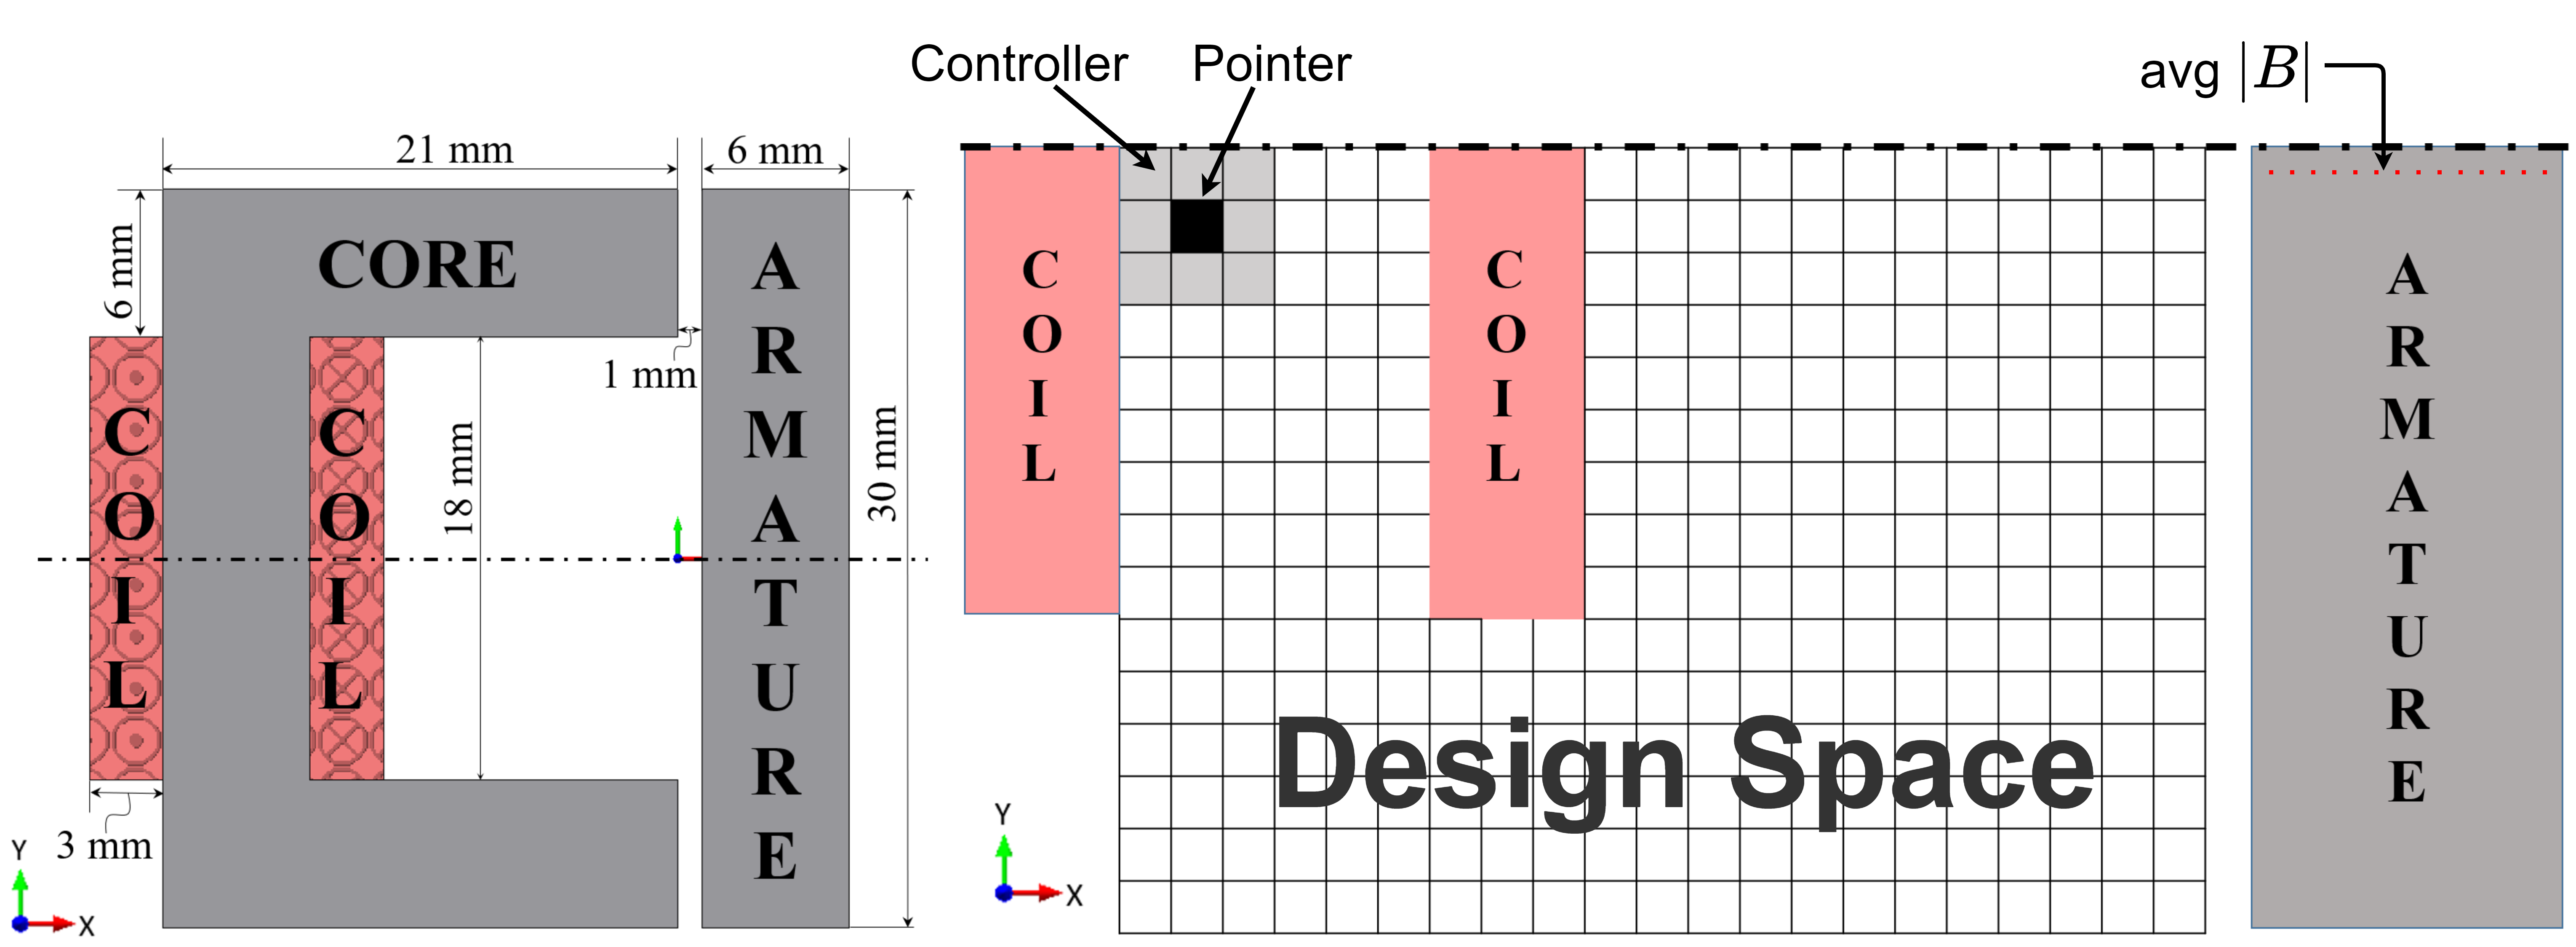
\includegraphics[width=\textwidth]{Figures/Ch_RL/c_core_conventional_design_domain.png}
    \caption{(a) Conventional C-core actuator (b) Design domain for half C-core with the controller ($3 \times 3$), pointer and performance measure.}
    \label{fig:RL_c_core_conventional_design_domain}
\end{figure}

\subsection{Results of Q-Learning}

The optimal geometry for a $3 \times 3$ SeqTO environment with a linear magnetic material is shown in Figure \ref{fig:DQN_results}. This result matches the geometry obtained through the GA and tabular TD-learning/Q-Learning algorithm (Figure \ref{subfig:td_linear_action_seq}).
The network uses the state representation similar to the one used for Tabular QL in Section \ref{subsubsec:MDP_Q_learning}. The memory buffer is populated with samples collected following a random policy. It was observed that starting with random sampling helps with the exploration on top of the $\epsilon$- greedy policy. Once sufficient random samples have been generated the learning phase of the QL-based agent starts. The results obtained match those obtained with the tabular QL algorithm in Section \ref{section:MDP_comparison_OnOFF_SeqTO}. The network takes about 950 episodes to converge to the optimal solution, requiring about 20,000 FE function calls in the process.

\begin{comment}
\begin{figure}[h!]
    \centering
    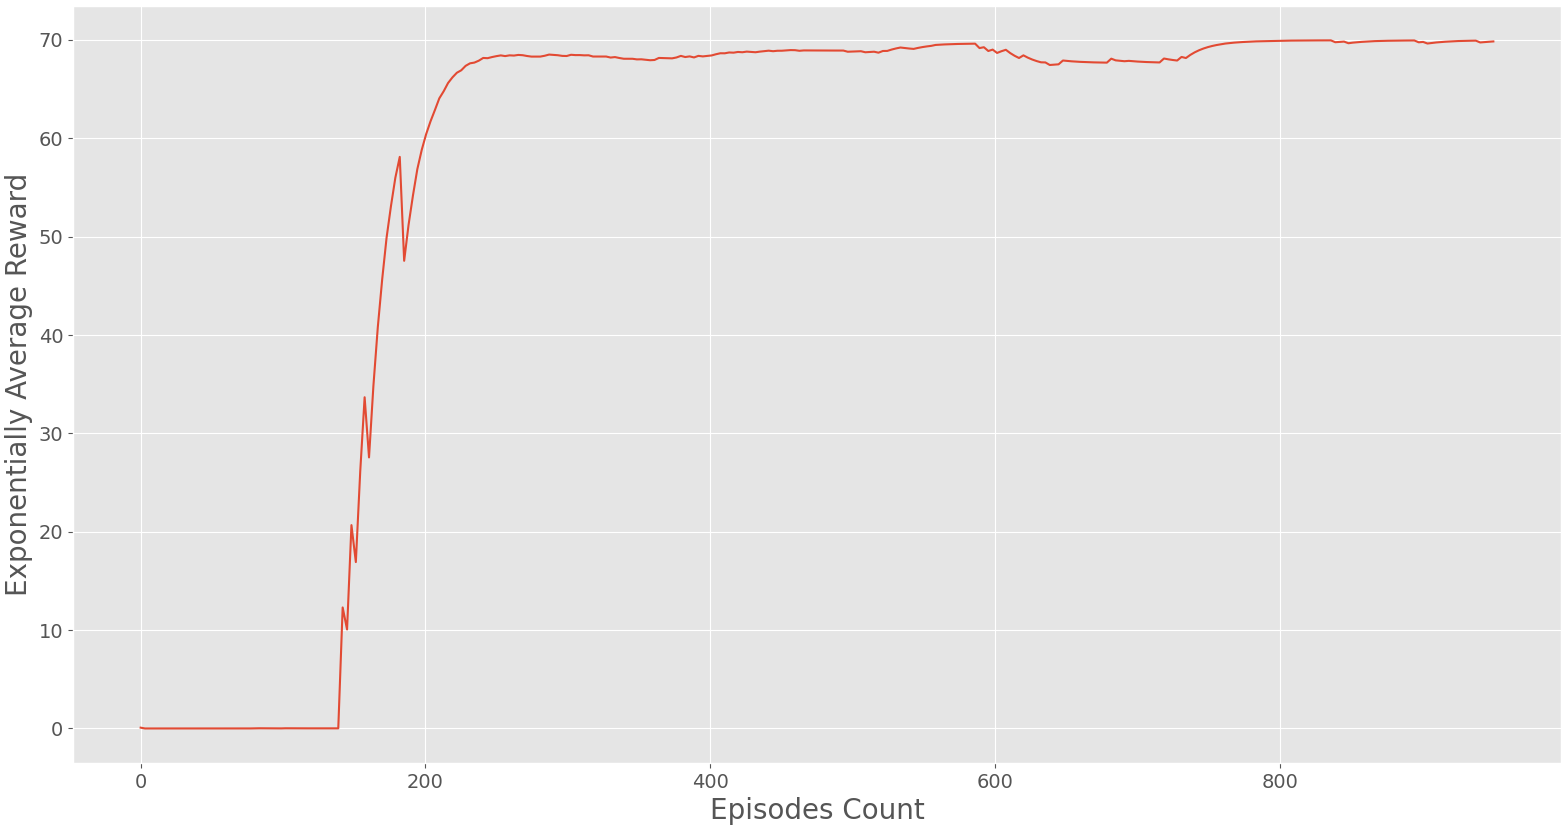
\includegraphics[width=\textwidth]{Figures/Ch_RL/1_Amps_QL.png}
    \caption{Caption}
    \label{fig:RL_1A_DQL_results}
\end{figure}

\begin{figure}{.45\textwidth}
    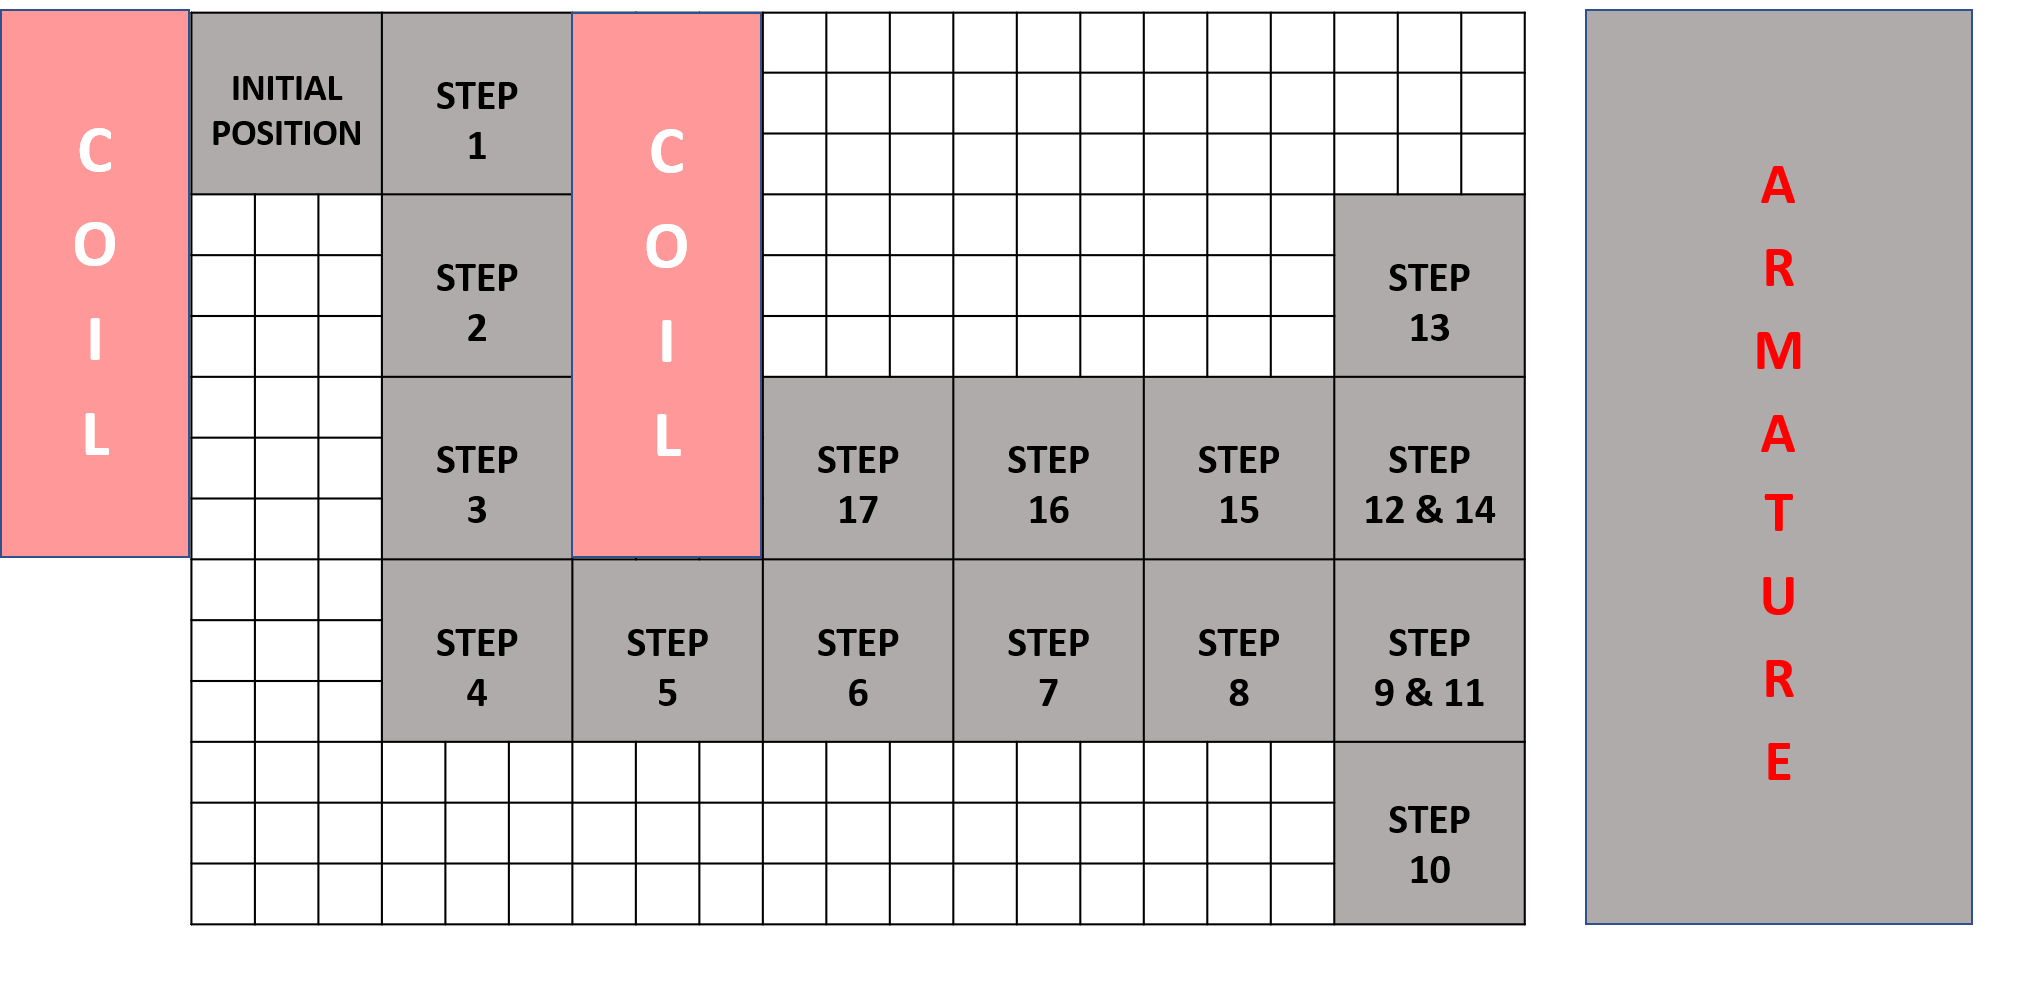
\includegraphics[width=\linewidth]{Figures/Ch_MDP/agent_result_TDlearning.png}
    \caption{The optimal solution and action sequence in a $3 \times 3$ linear environment}
    \label{fig:RL_td_linear_action_seq}  
\end{figure}
\end{comment}

\begin{figure}[h!]
    \centering
        \begin{subfigure}{.45\textwidth}
        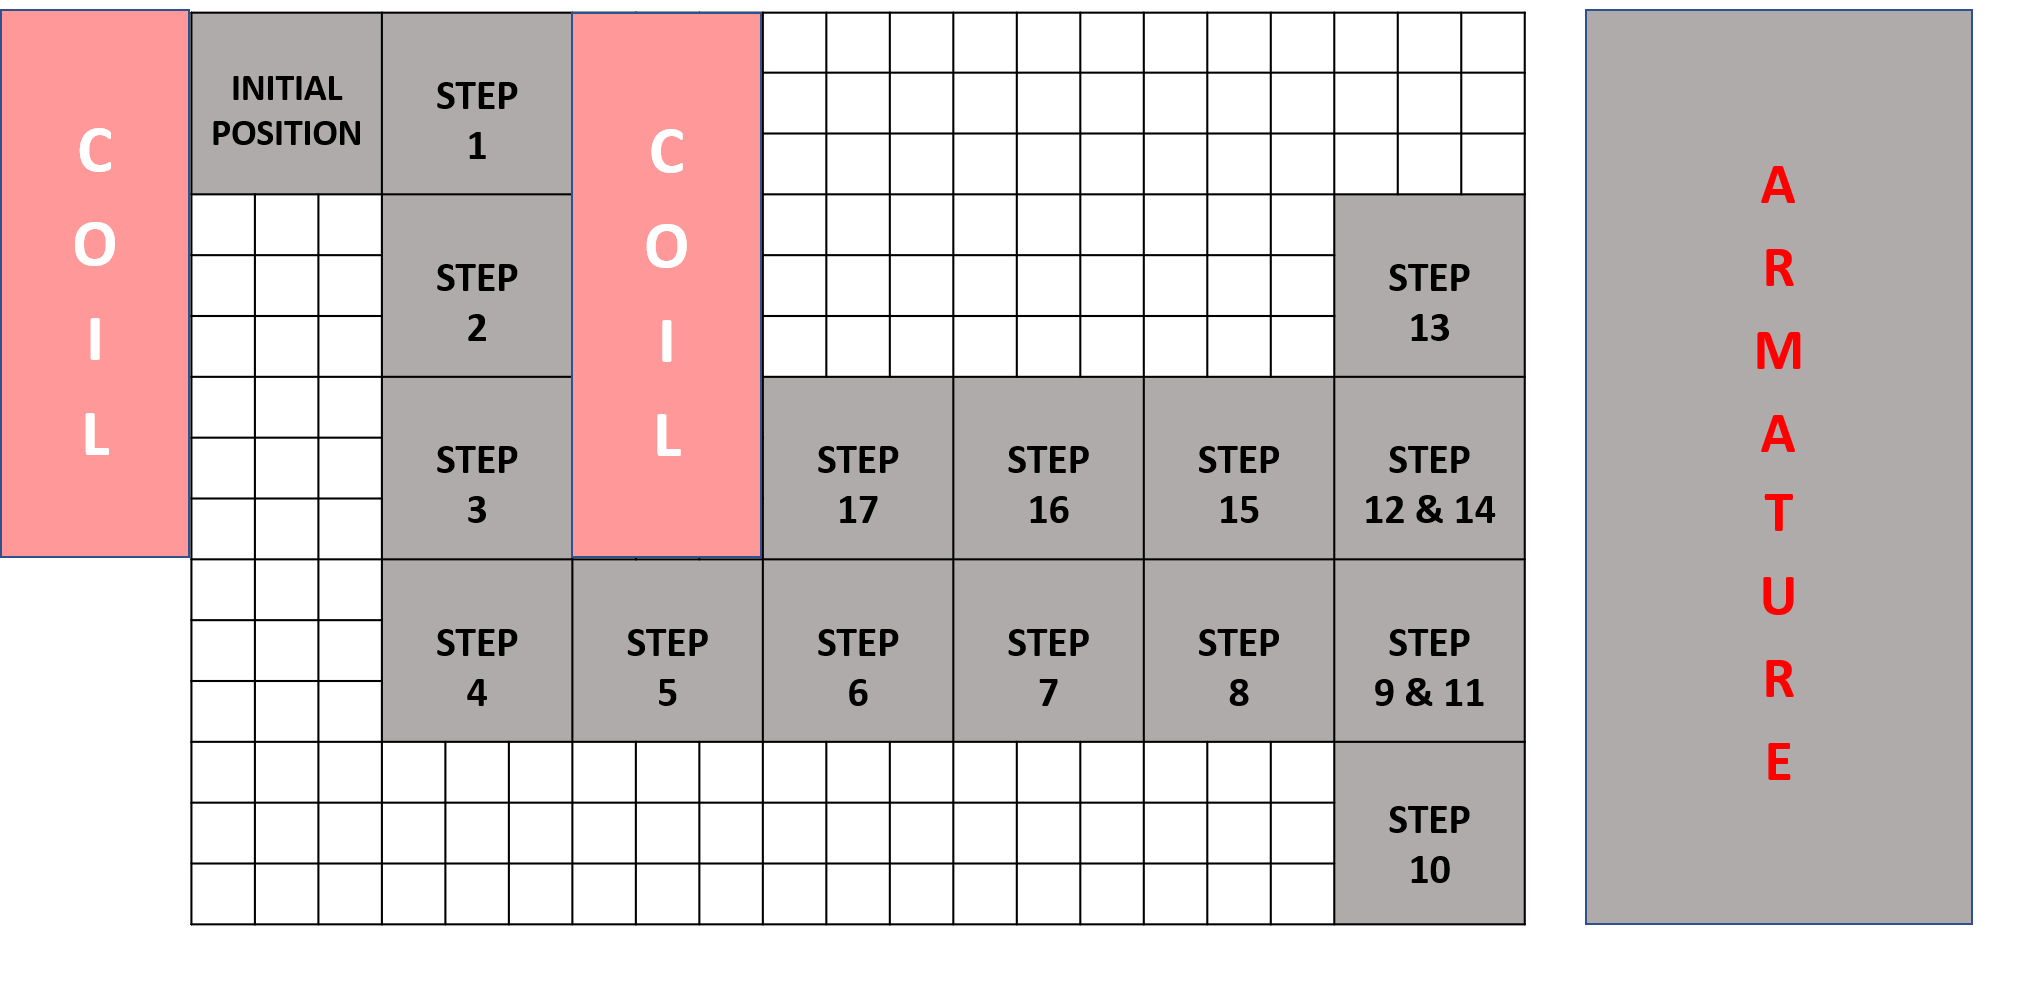
\includegraphics[width=\linewidth]{Figures/Ch_MDP/agent_result_TDlearning.png}
        \caption{Convergence results for 1.0 Amps using Deep Q-learning algorithm.}
        \label{subfig:RL_convergence_QL_1Amps}  
    \end{subfigure}
    \begin{subfigure}{.45\textwidth}
        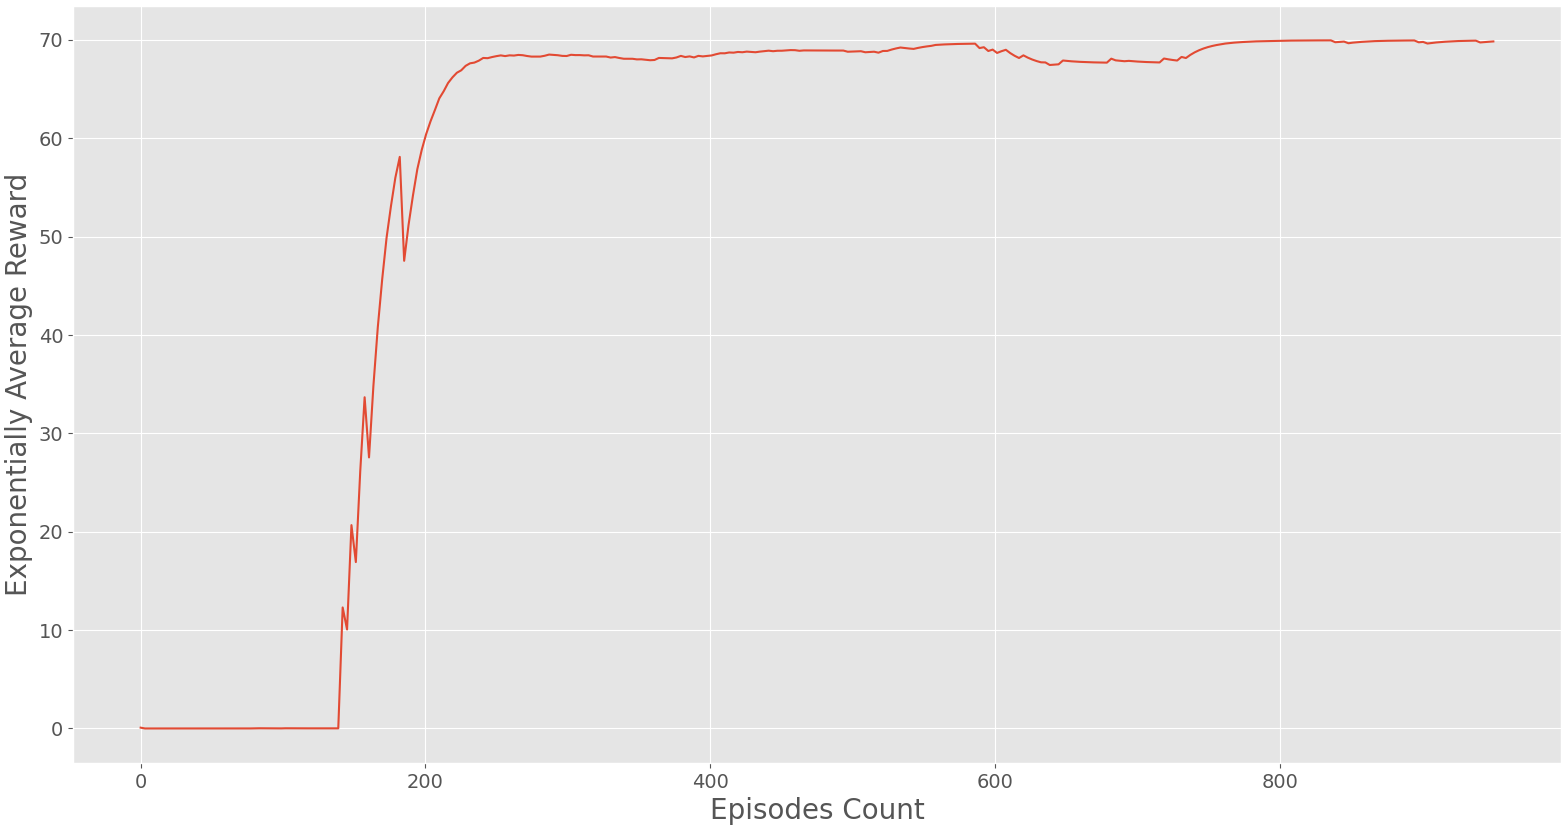
\includegraphics[width=\textwidth]{Figures/Ch_RL/1_Amps_QL.png}
        \caption{The optimal solution and action sequence in a $3 \times 3$ linear environment}
        \label{subfig:RL_1A_DQL_results}
    \end{subfigure}
    \caption{Optimal geometry of C-core with Deep Q-Learning, using a $3 \times 3$ controller filling linear iron material.}
    \label{fig:DQN_results}
\end{figure}

\section{Modifications to SeqTo-v1 environment}
\label{section:RL_MDP}

The RL task needs to be formulated as a Markov decision process (MDP) \parencite{bellman1957markovian}, similar to the one discussed in Chapter \ref{chapter:4_MDP}. Briefly speaking, an MDP comprises of four parts $\mathdc{S}$, $\mathdc{A}$, $\mathdc{P}$, $\mathdc{R}$, where $\mathdc{P}$ is the transition probability function. The description of the transition probability functions $\mathdc{P}$ is omitted because any state-action pair deterministically leads to a unique next state. The reward is based on the increase or decrease of the magnetic field distribution at the point near the middle of the armature as shown in the armature.

Although the MDP discussed in Chapter \ref{chapter:4_MDP}, Section \ref{section:MDP_MDP} is suitable for deploying RL algorithms, the current discussion extends the MDP to account for more complex geometries while keeping the computational cost low.
Further, certain modifications are to be made to enable the state to contain more relevant information, that can be useful for the agent to make a decision. 

Additionally, up until now only a $3 \times 3$ controller has been used with both the tabular and function approximator form of Q-Learning. This limitation does not allow the generation of complex structures.
If the same state representation and MDP is to be used with a controller of the size of $1 \times 1$, the number of steps needed to achieve an optimal structure with the amount of given material will be overwhelming, resulting in high number of simulations.
Additionally, a state should include as much relevant numerical data of the design as possible. The MDP formulated in Section \ref{section:MDP_MDP}, was ideal for tabular algorithms as it consists of only integer encoding for the state representation. 

To mitigate these issues, a state representation that holds more information and an action space that is more complicated and at the same time offers more flexibility to the controller is developed and this modified environment will be referred to as SeqTO-v2. SeqTO-v2 will include different ways of encoding useful numerical information into the state representation. This change is made for both the C-core problem and SynRM geometry. Although for SynRM no changes are made in the action dimensionality (as compared to SeqTO-v1), the techniques mentioned can easily be adopted. These changes are incorporated to balance the granularity of the solution and limit the number of electromagnetic simulations in an episode of training. The state representation used in Chapter \ref{chapter:4_MDP} is shown in Figure \ref{fig:RL_state_repr_original}. In addition to the material distribution and coils, an alternate representation involves additional information of the magnitude of the magnetic field distribution in the airgap, as shown in Figure \ref{fig:RL_state_repr_2}. Another possibility is providing information related to the magnetic field distribution over the complete design space. This is shown in Figure \ref{fig:RL_state_repr_3_Bfield}, where the information is stored in channels as the first channel of dimensions ($W \times H$) consisting of the material distribution along with the spatial location, current magnitude, and the number of turns for the coil. The second channel consists of the magnitude of the magnetic field distribution over the same spatial dimension as the first channel of a multi-channel or 3D representation. This is the most complete state representation of the three.  

\begin{figure}[h!]
\centering
\begin{minipage}{.45\textwidth}
  \centering
  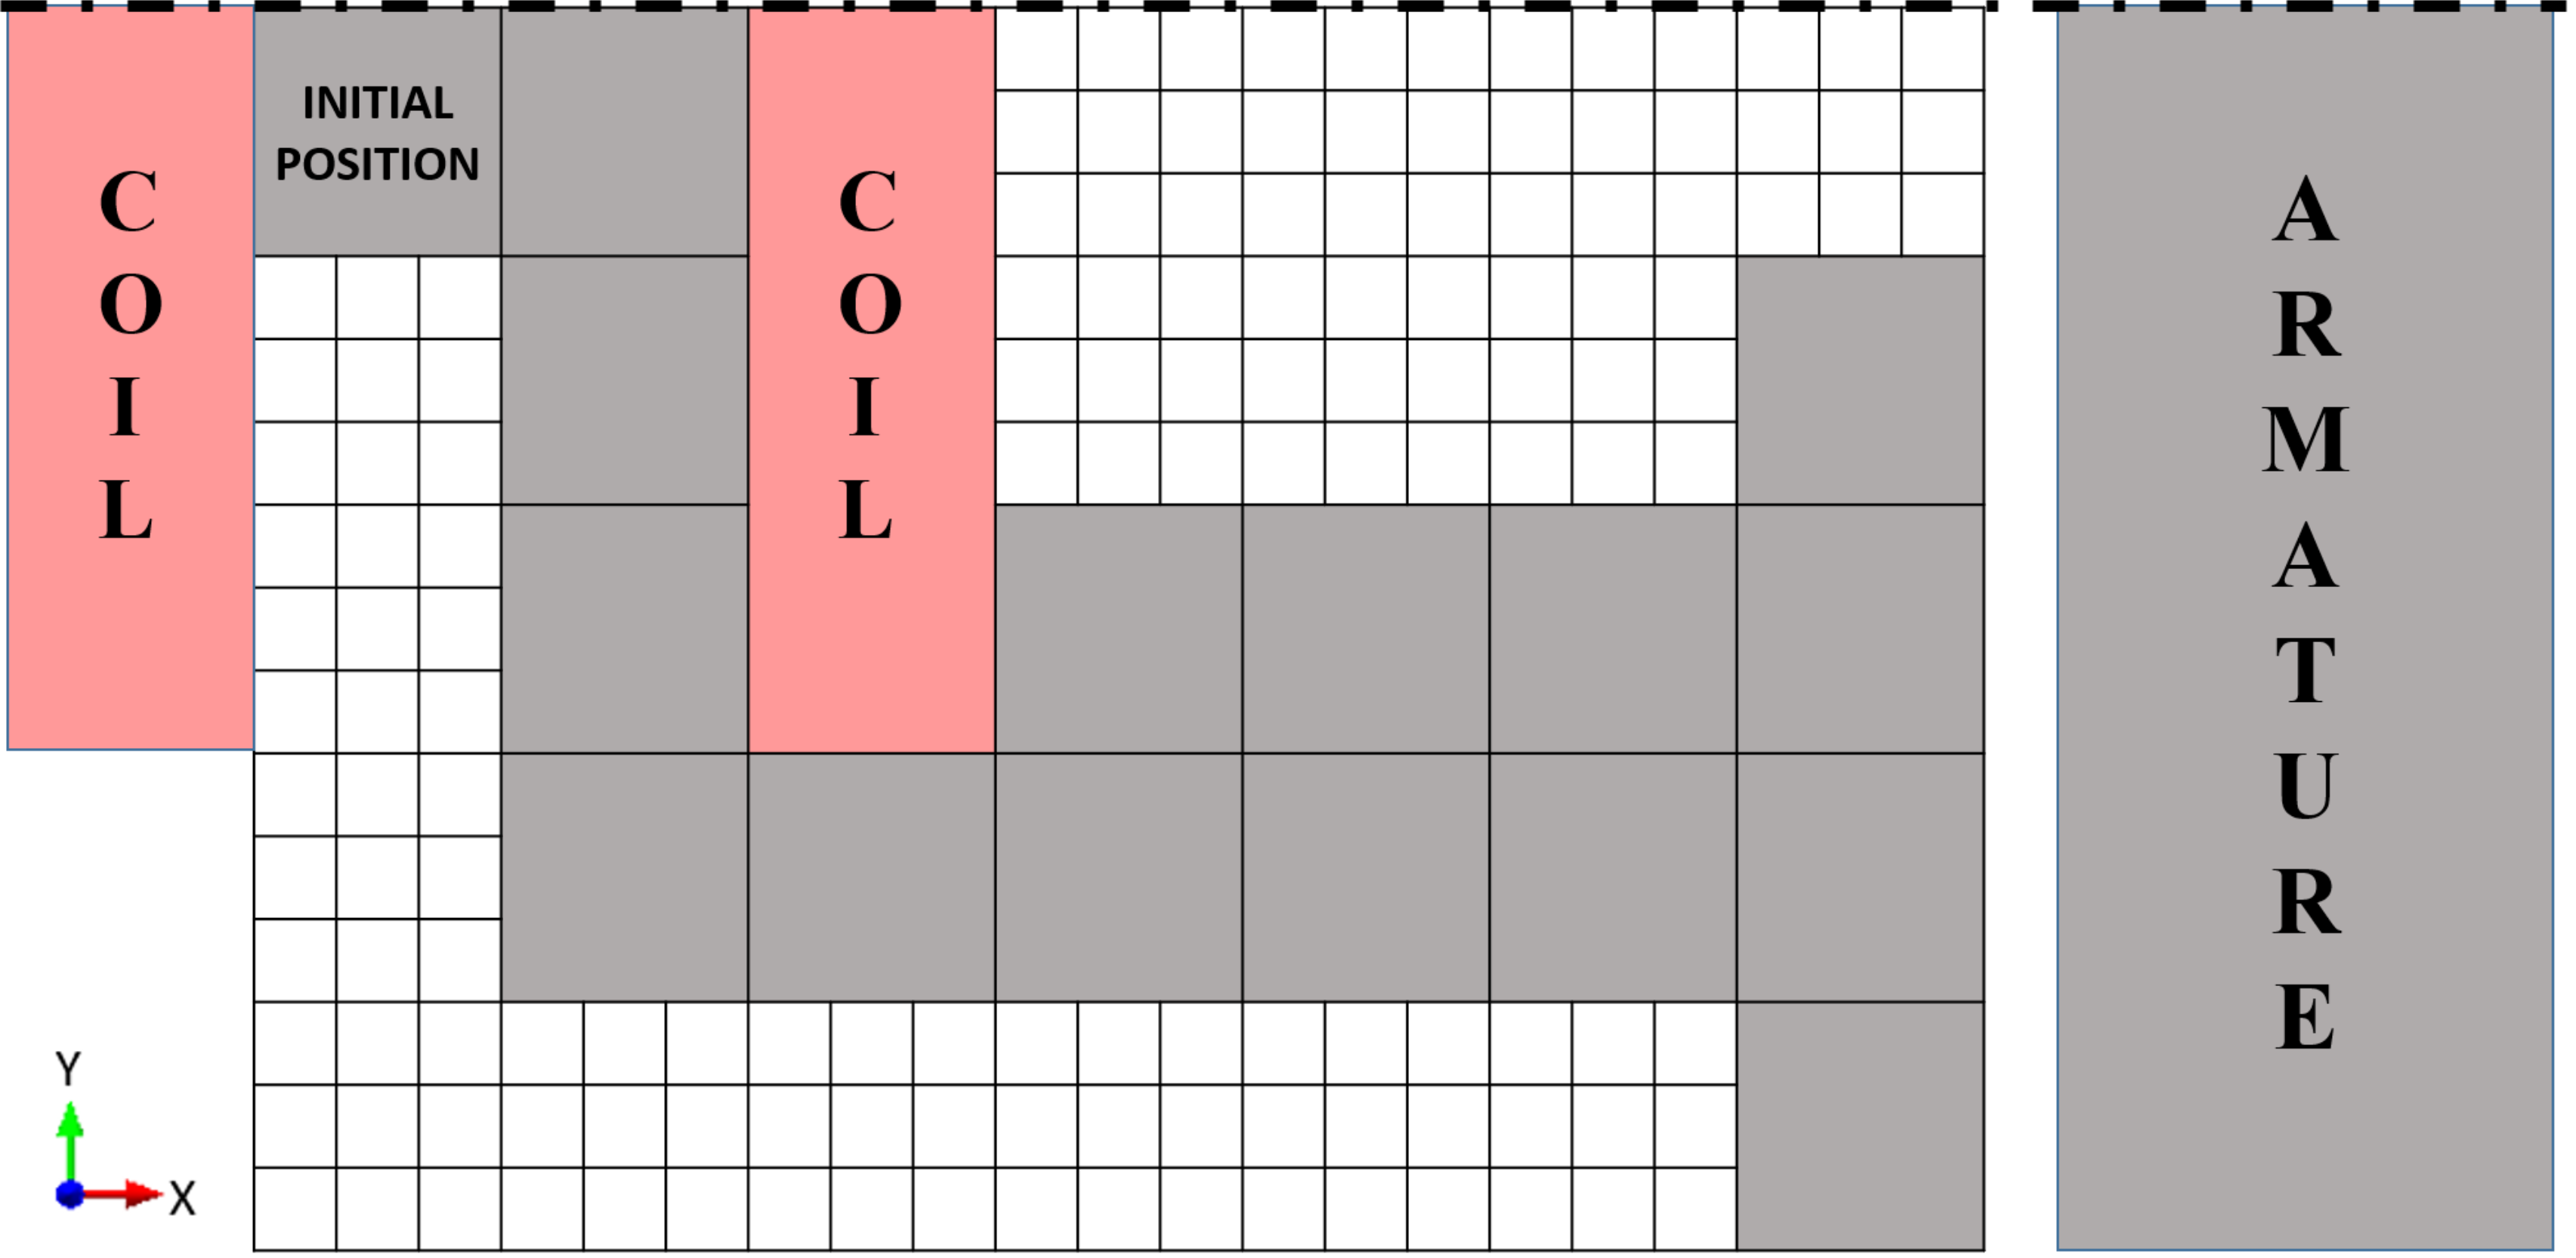
\includegraphics[width=0.8\linewidth]{Figures/Ch_MDP/state_repr_1.png}
  \captionof{figure}{Discrete design domain as the state space}
  \label{fig:RL_state_repr_original}
\end{minipage}%
\begin{minipage}{.45\textwidth}
  \centering
  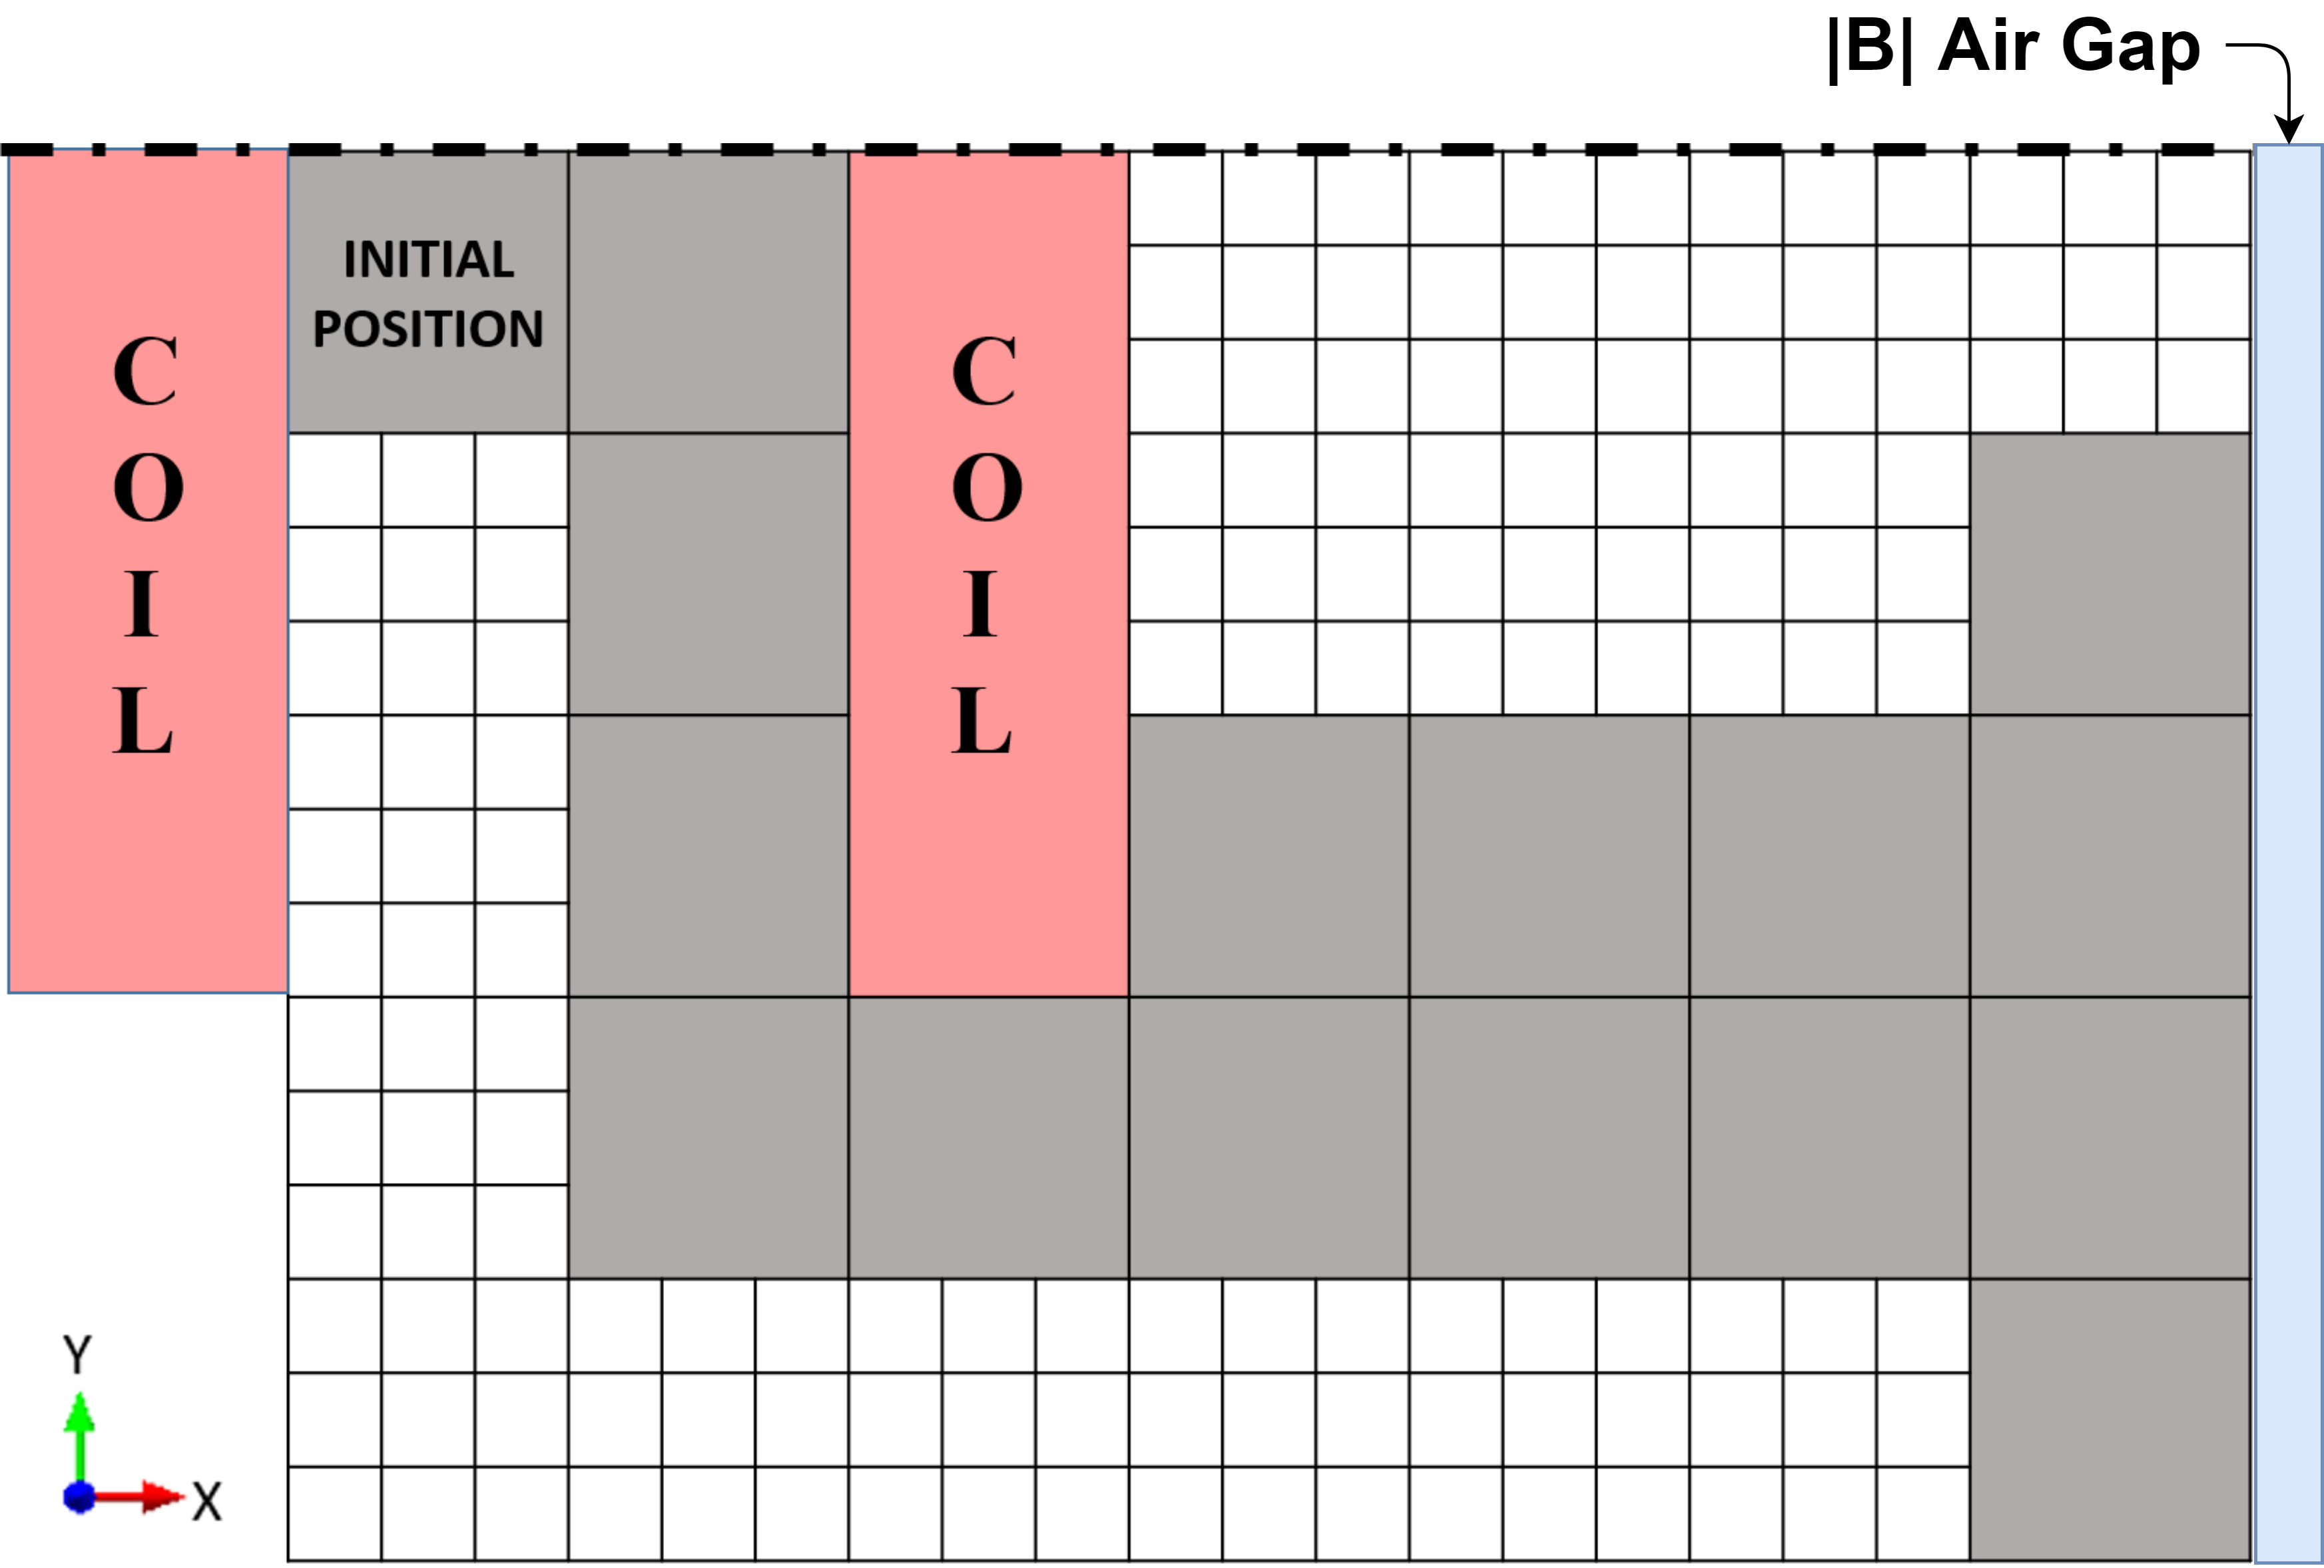
\includegraphics[width=0.8\linewidth]{Figures/Ch_MDP/state_repr_2.png}
  \captionof{figure}{Discrete design domain with the $|B|_{airgap}$ as the state space}
  \label{fig:RL_state_repr_2}
\end{minipage}
\end{figure}

\begin{figure}[h!]
    \centering
    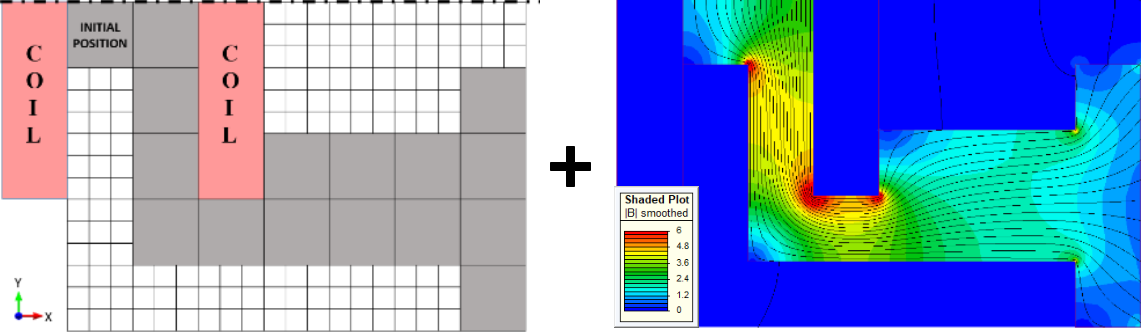
\includegraphics[width=0.75\textwidth]{Figures/Ch_MDP/state_repr_3_mdp.png}
    \caption{Discrete design domain  along with the $|B|$ in the design space as the state space}
    \label{fig:RL_state_repr_3_Bfield}
\end{figure}

As for the action space, it initially consists of only four options which were discussed in Chapter \ref{chapter:4_MDP}, Section \ref{section:MDP_Sequence_based_controller} and shown in Figure \ref{fig:MDP_controller_movement}. The action space for the controller is increased by four to a total of eight such that the controller now has the ability to place not only $3 \times 3$ block of data, but additional option including $3 \times 1$, $1 \times 3$, $3 \times 2$, $2 \times 3$ along with several other combinations as shown in Figure \ref{fig:RL_agent_movement}. Effectively, the controller now has the capability of placing from a minimum of 3 ($1 \times 3$) to a maximum of 9 ($3 \times 3$) in a single step, using an additional set of actions labelled as `soft' actions. The complete set of actions, available to the controller at any step in an episode are mentioned in Table \ref{tab:RL_action_options} and the operation of these actions is shown in Figure \ref{fig:RL_agent_movement}. 

\begin{table}[h!]
\centering
\begin{tabular}{|c|c||c|c|}
\hline
\textbf{} & \textbf{Action} & \textbf{} & \textbf{Action}\\ \hline \hline
1         & Soft Up         & 5     & Up\\ \hline
2         & Soft Down       & 6     & Down \\ \hline
3         & Soft Right      & 7     & Right\\ \hline
4         & Soft Left       & 8     & Left\\ \hline
\end{tabular}
\caption{Evolved action space of the controller (SeqTO-v2).}
\label{tab:RL_action_options}
\end{table}

\begin{figure}[h!]
    \centering
    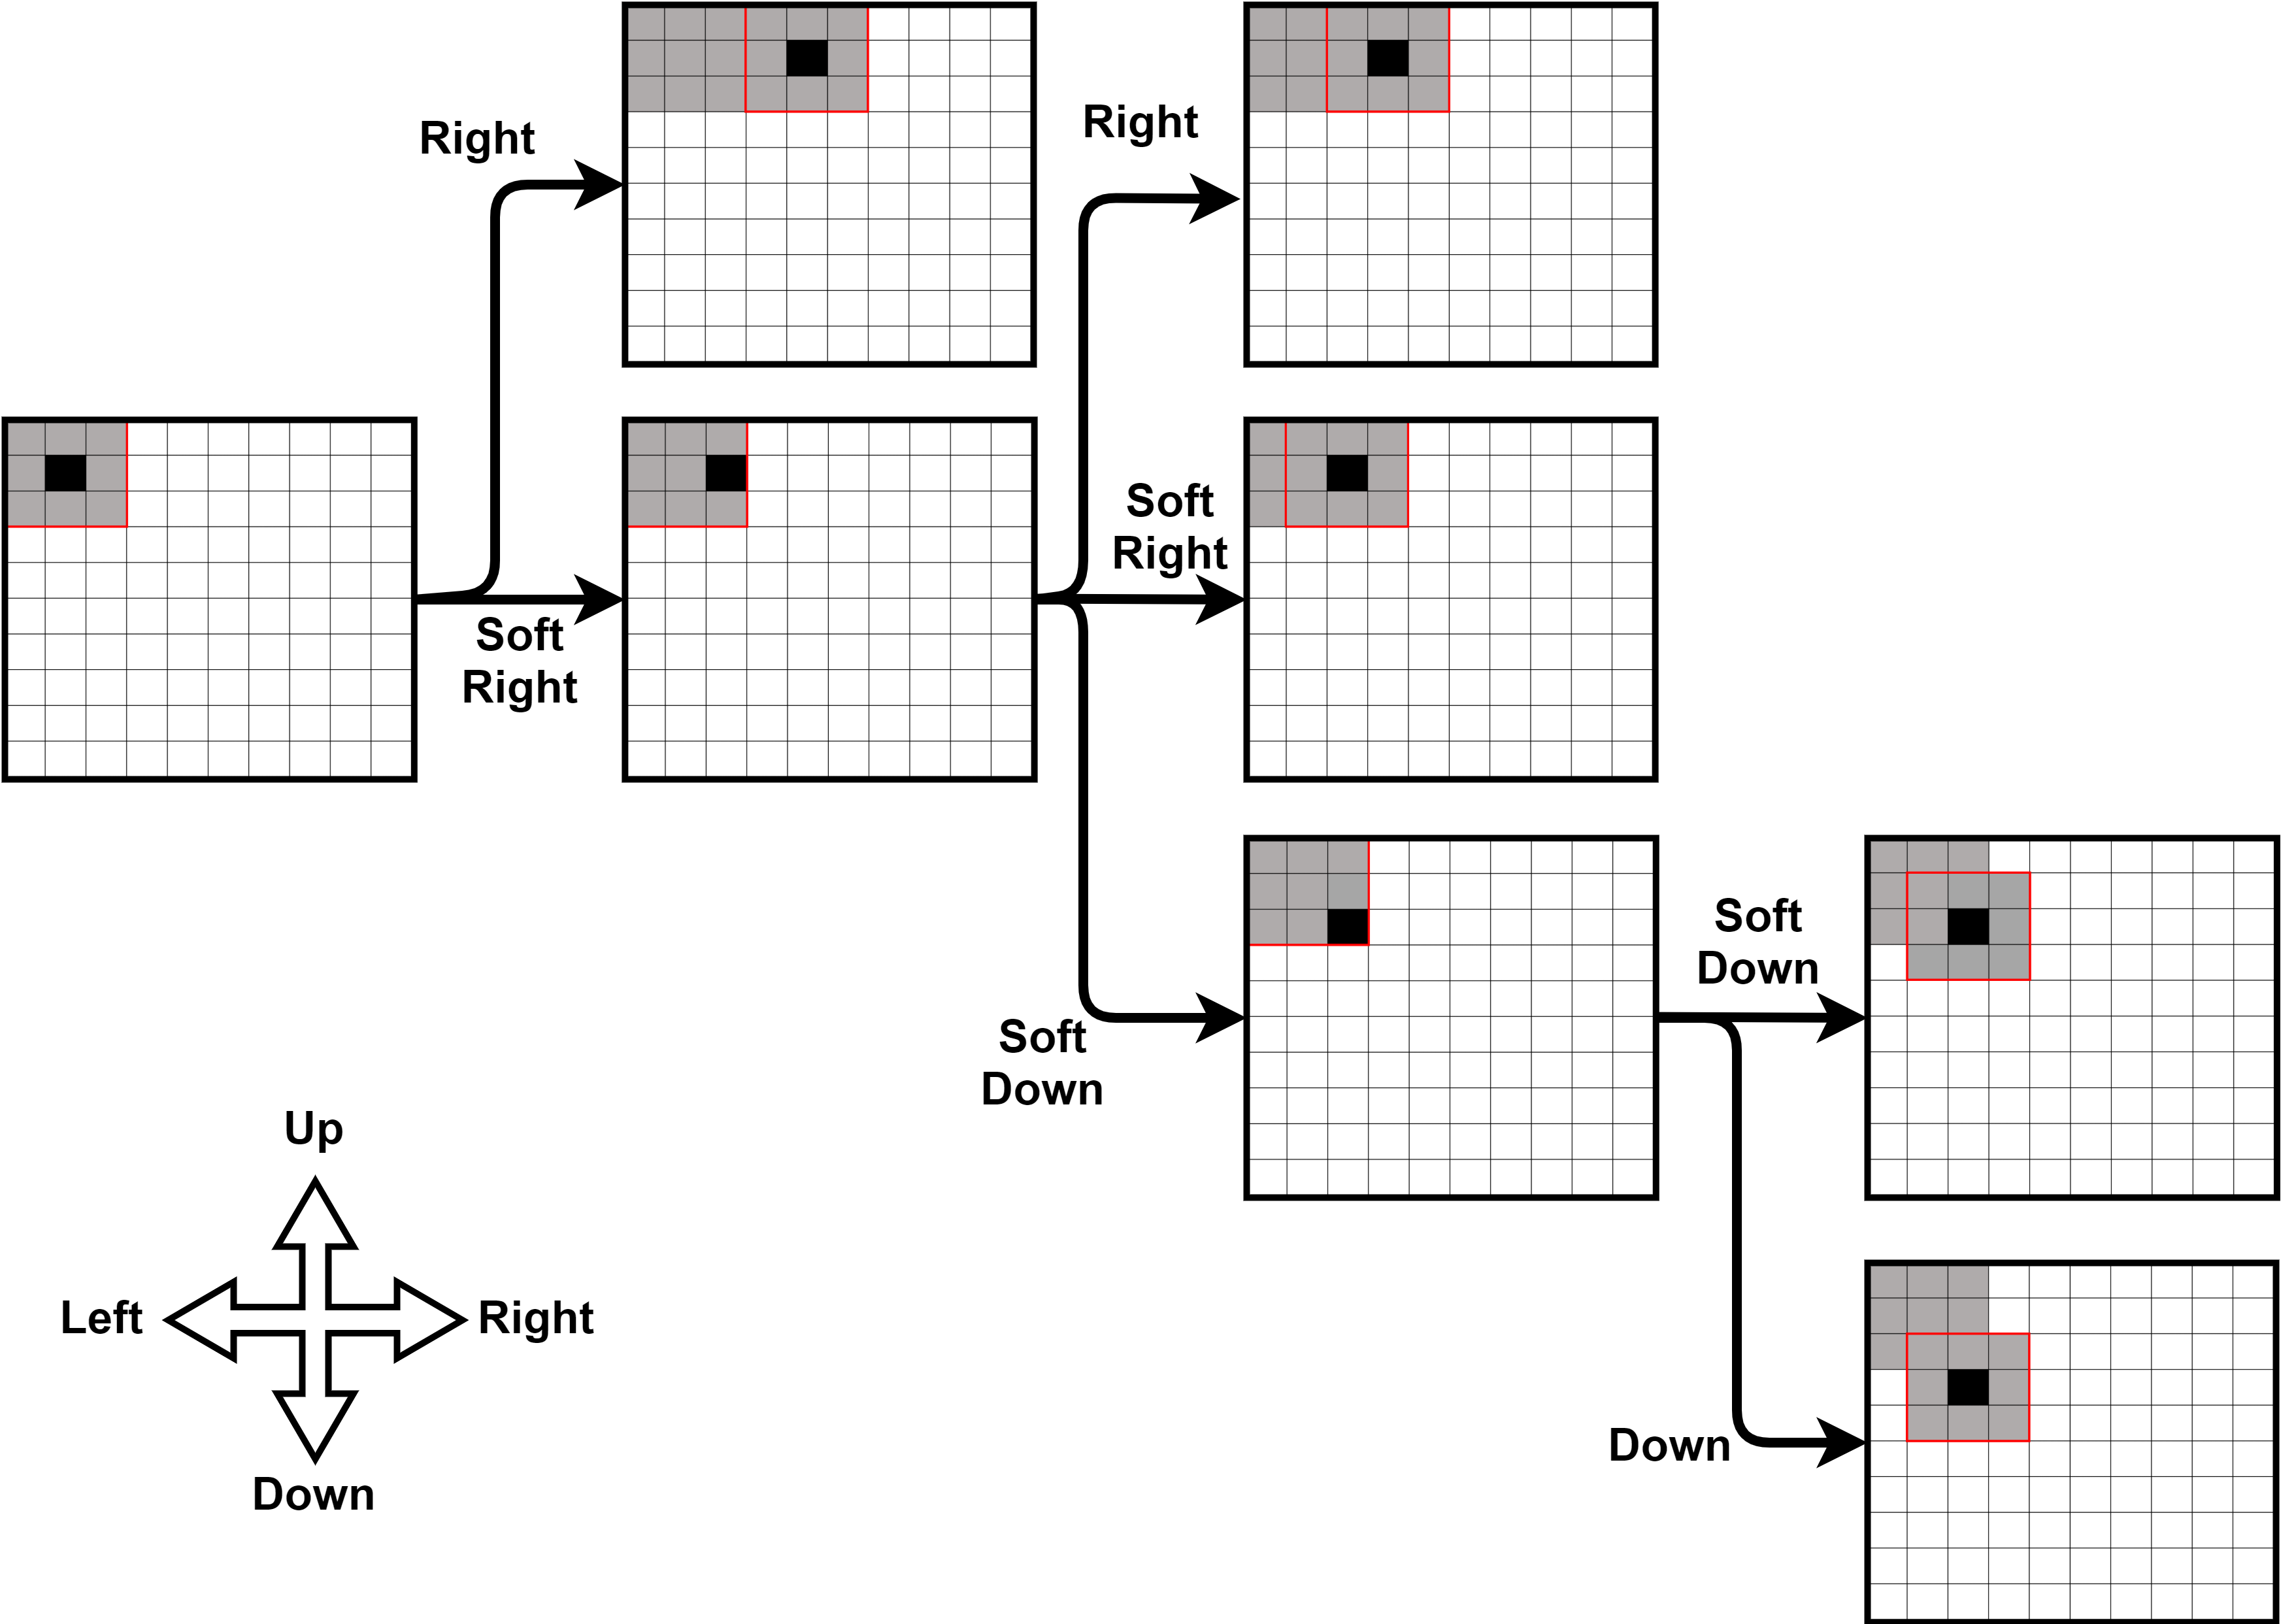
\includegraphics[width=\textwidth]{Figures/Ch_RL/C_core_movement_final400.png}
    \caption{Agent Movement with SeqTO-v2 controller.}
    \label{fig:RL_agent_movement}
\end{figure}

Although the Markov property states that there must not be any useful information in previous states \parencite{markov1951teoriya}. This property can be relaxed, similar to \cite{silver2017mastering}. In the case of using a single design domain information at an instant `$t$' as our state, we are breaking the Markov property because previous frames could be used to infer the previous changes made by the agent and can help with the differentiation if the agent took any good or bad actions there. An agent trying to enter the coil space is bad and can be differentiated here, as shown in Figure \ref{fig:RL_coil_error2}. This is dealt by bringing some of the history into the state. 

\begin{figure}[h!]
    \centering
    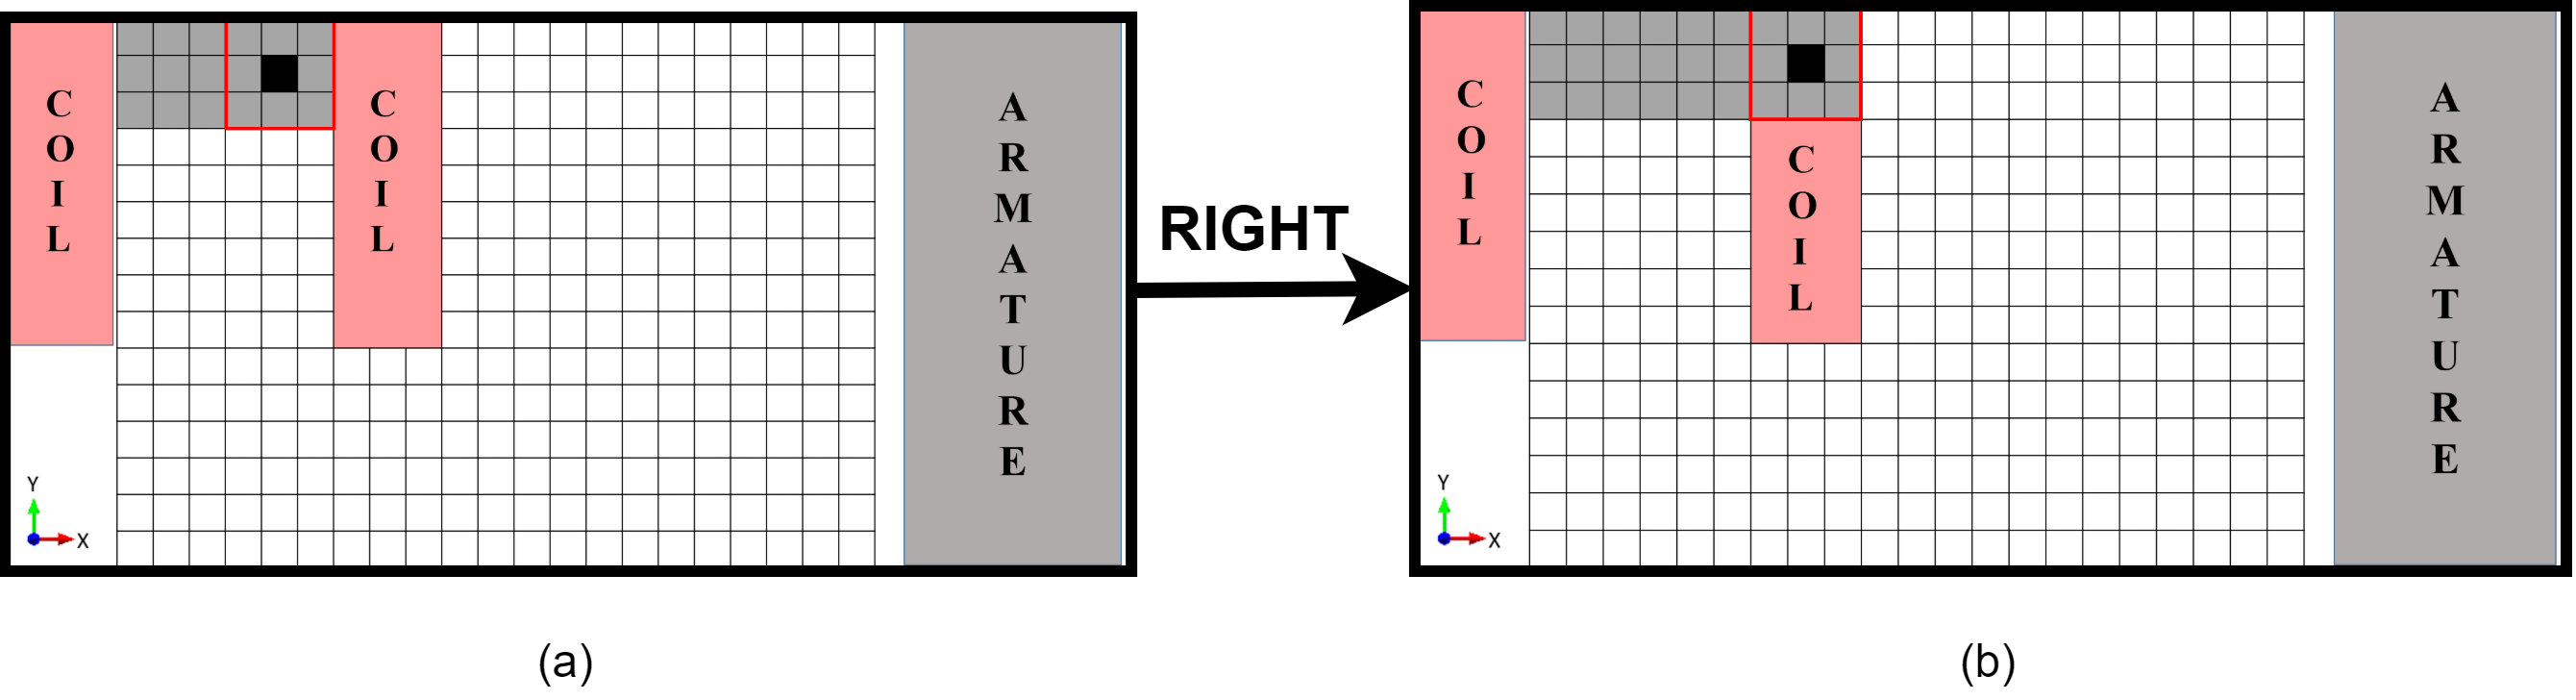
\includegraphics[width=\textwidth]{Figures/Ch_RL/Coil_error.png}
    \caption{Possibility of a design error due to the controller moving out of the designated design space.}
    \label{fig:RL_coil_error2}
\end{figure}

\section{Policy Gradient}

A Q-Learning algorithm learns by trying to find each state’s action-value function (Q-Value function). Its entire learning procedure is based on the principle of figuring out the quality of each possible action and select the best possible action, according to the learned knowledge. So Q-Learning tries to have complete and unbiased knowledge of all possible moves, which is also its most major drawback, as this requires a significant number of attempts of each possible state and action combination. 

\begin{align}
    \text{Training} \Longrightarrow \theta \longrightarrow Q(s,a) \longrightarrow \pi
\end{align}

Policy Gradient (PG) is a different paradigm of RL algorithm that learns more robustly, by trying not to evaluate the value of each action, but by simply evaluating which action it should prefer.
The learning cycle of a PG algorithm is shorter, skipping the Q-Value function part:

\begin{align}
    \text{Training} \Longrightarrow \theta \longrightarrow \pi
\end{align}

\begin{figure}[h!]
    \centering
    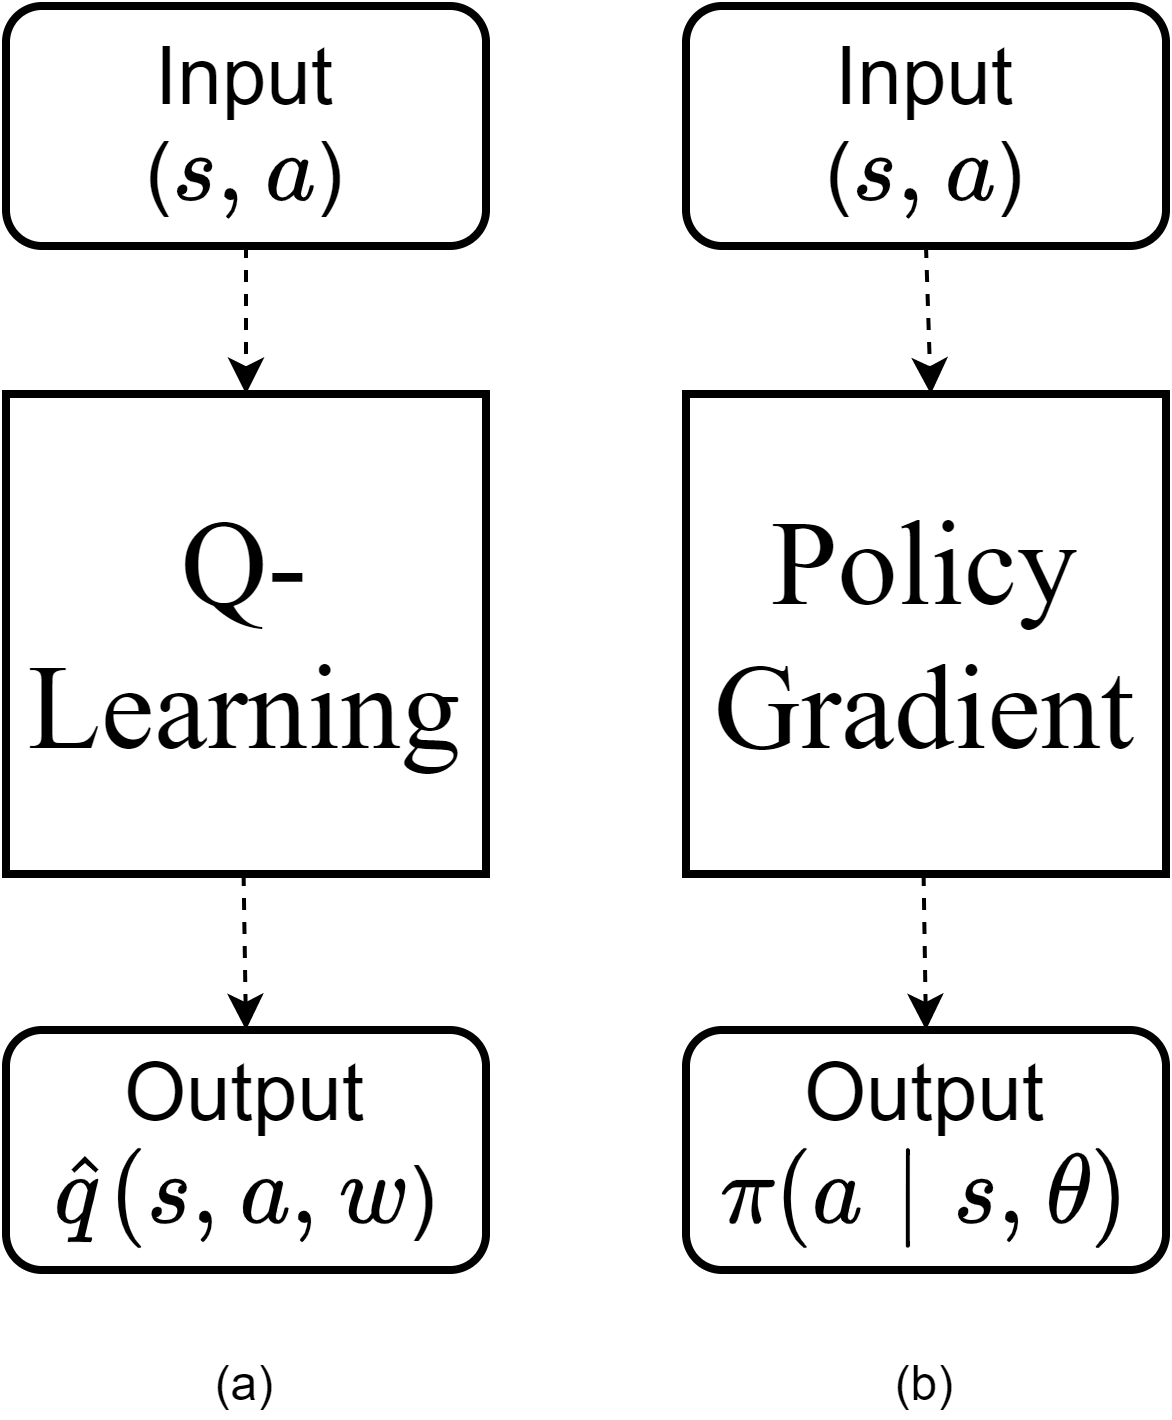
\includegraphics[width=0.35\textwidth]{Figures/Ch_RL/QL_vs_PG.png}
    \caption{Q-learning vs Policy Gradient Method}
    \label{fig:RL_QLvsPG}
\end{figure}

This means that the network will directly output the probability of selecting each action, skipping the extra calculation. This also allows the PG algorithm to be more robust. The update for the Q-learning algorithm was based on either the return ($G_t$) or the bootstrapped action value ($R + Q(s', a')$). In PG, a metric called the ``performance measure" (represented by the term $J$) will be responsible for making the changes in the weights of the neural net.

\begin{align}
    \theta_{t+1} = \theta_t + \alpha \nabla J(\theta_t)
\end{align}

A simple way of analyzing the performance ($J(\theta)$) is to measure all the rewards seen by the agent, similar to the return ($G_t$). The rewards accumulated in an episode is a good performance measurement since the agent’s sole purpose is to maximize its overall collected rewards. This can be calculated as:

\begin{align}
    J(\theta) = G(t) \approx \sum_a \Big(Q(s_0,a) \times p(a|s_0)\Big) \label{eqn:RL_performance_measure}
\end{align}

\begin{comment}
This is the sum of all Q-Values of the initial state $s_0$, multiplied by probability to select each action. This exactly our expected overall reward for an entire episode. This summation over all Q-Values of a certain state multiplied by their probabilities is called the state’s Value Function and is denoted as $V(s)$. A state’s Value Function is a measure of the expected reward from state $s$ and till the end of the episode, without knowing the action that will be chosen by the agent. Essentially, in eqn \ref{eqn:RL_performance_measure}, the initial state's Value function ($V(s)$ is defined as the performance measure: $J = V(s_0)$.

Once $J$ is defined, the next step will be to calculate its gradient. This involves some complex math, as $J$ depends on the probability of action selection $p(a)$, which is derived from the policy $\pi$ - but $\pi$ depends on $J$, since this is how we defined it. 
\end{comment}

Next, the weights of the neural network are to be optimized with respect to the performance criteria. It should be noted $J(\theta)$ depends on the probability of action selection $p(a)$, which is derived from the policy ($\pi$). The gradient of $J(\theta)$ is calculated and the weights are updated by:

\begin{align}
    \nabla_{\theta} J = G_t \cdot \nabla log (\pi(a_t | s_t; \theta))
\end{align}

where $G_t$ is the total accumulated reward from step `$t$' till the end of the episode. 
The change in the weights of the policy network is represented as:

\begin{align}
    \theta_{t+1} = \theta_t + \alpha (G_t \cdot \nabla log (\pi(a_t | s_t; \theta))) \label{eqn:RL_PG_5_13}
\end{align}

where $\alpha$ is the learning rate and $\theta$ is the representation of the parameters (weights) associated with the neural network of the policy ($\pi$).

\begin{figure}[h!]
    \centering
    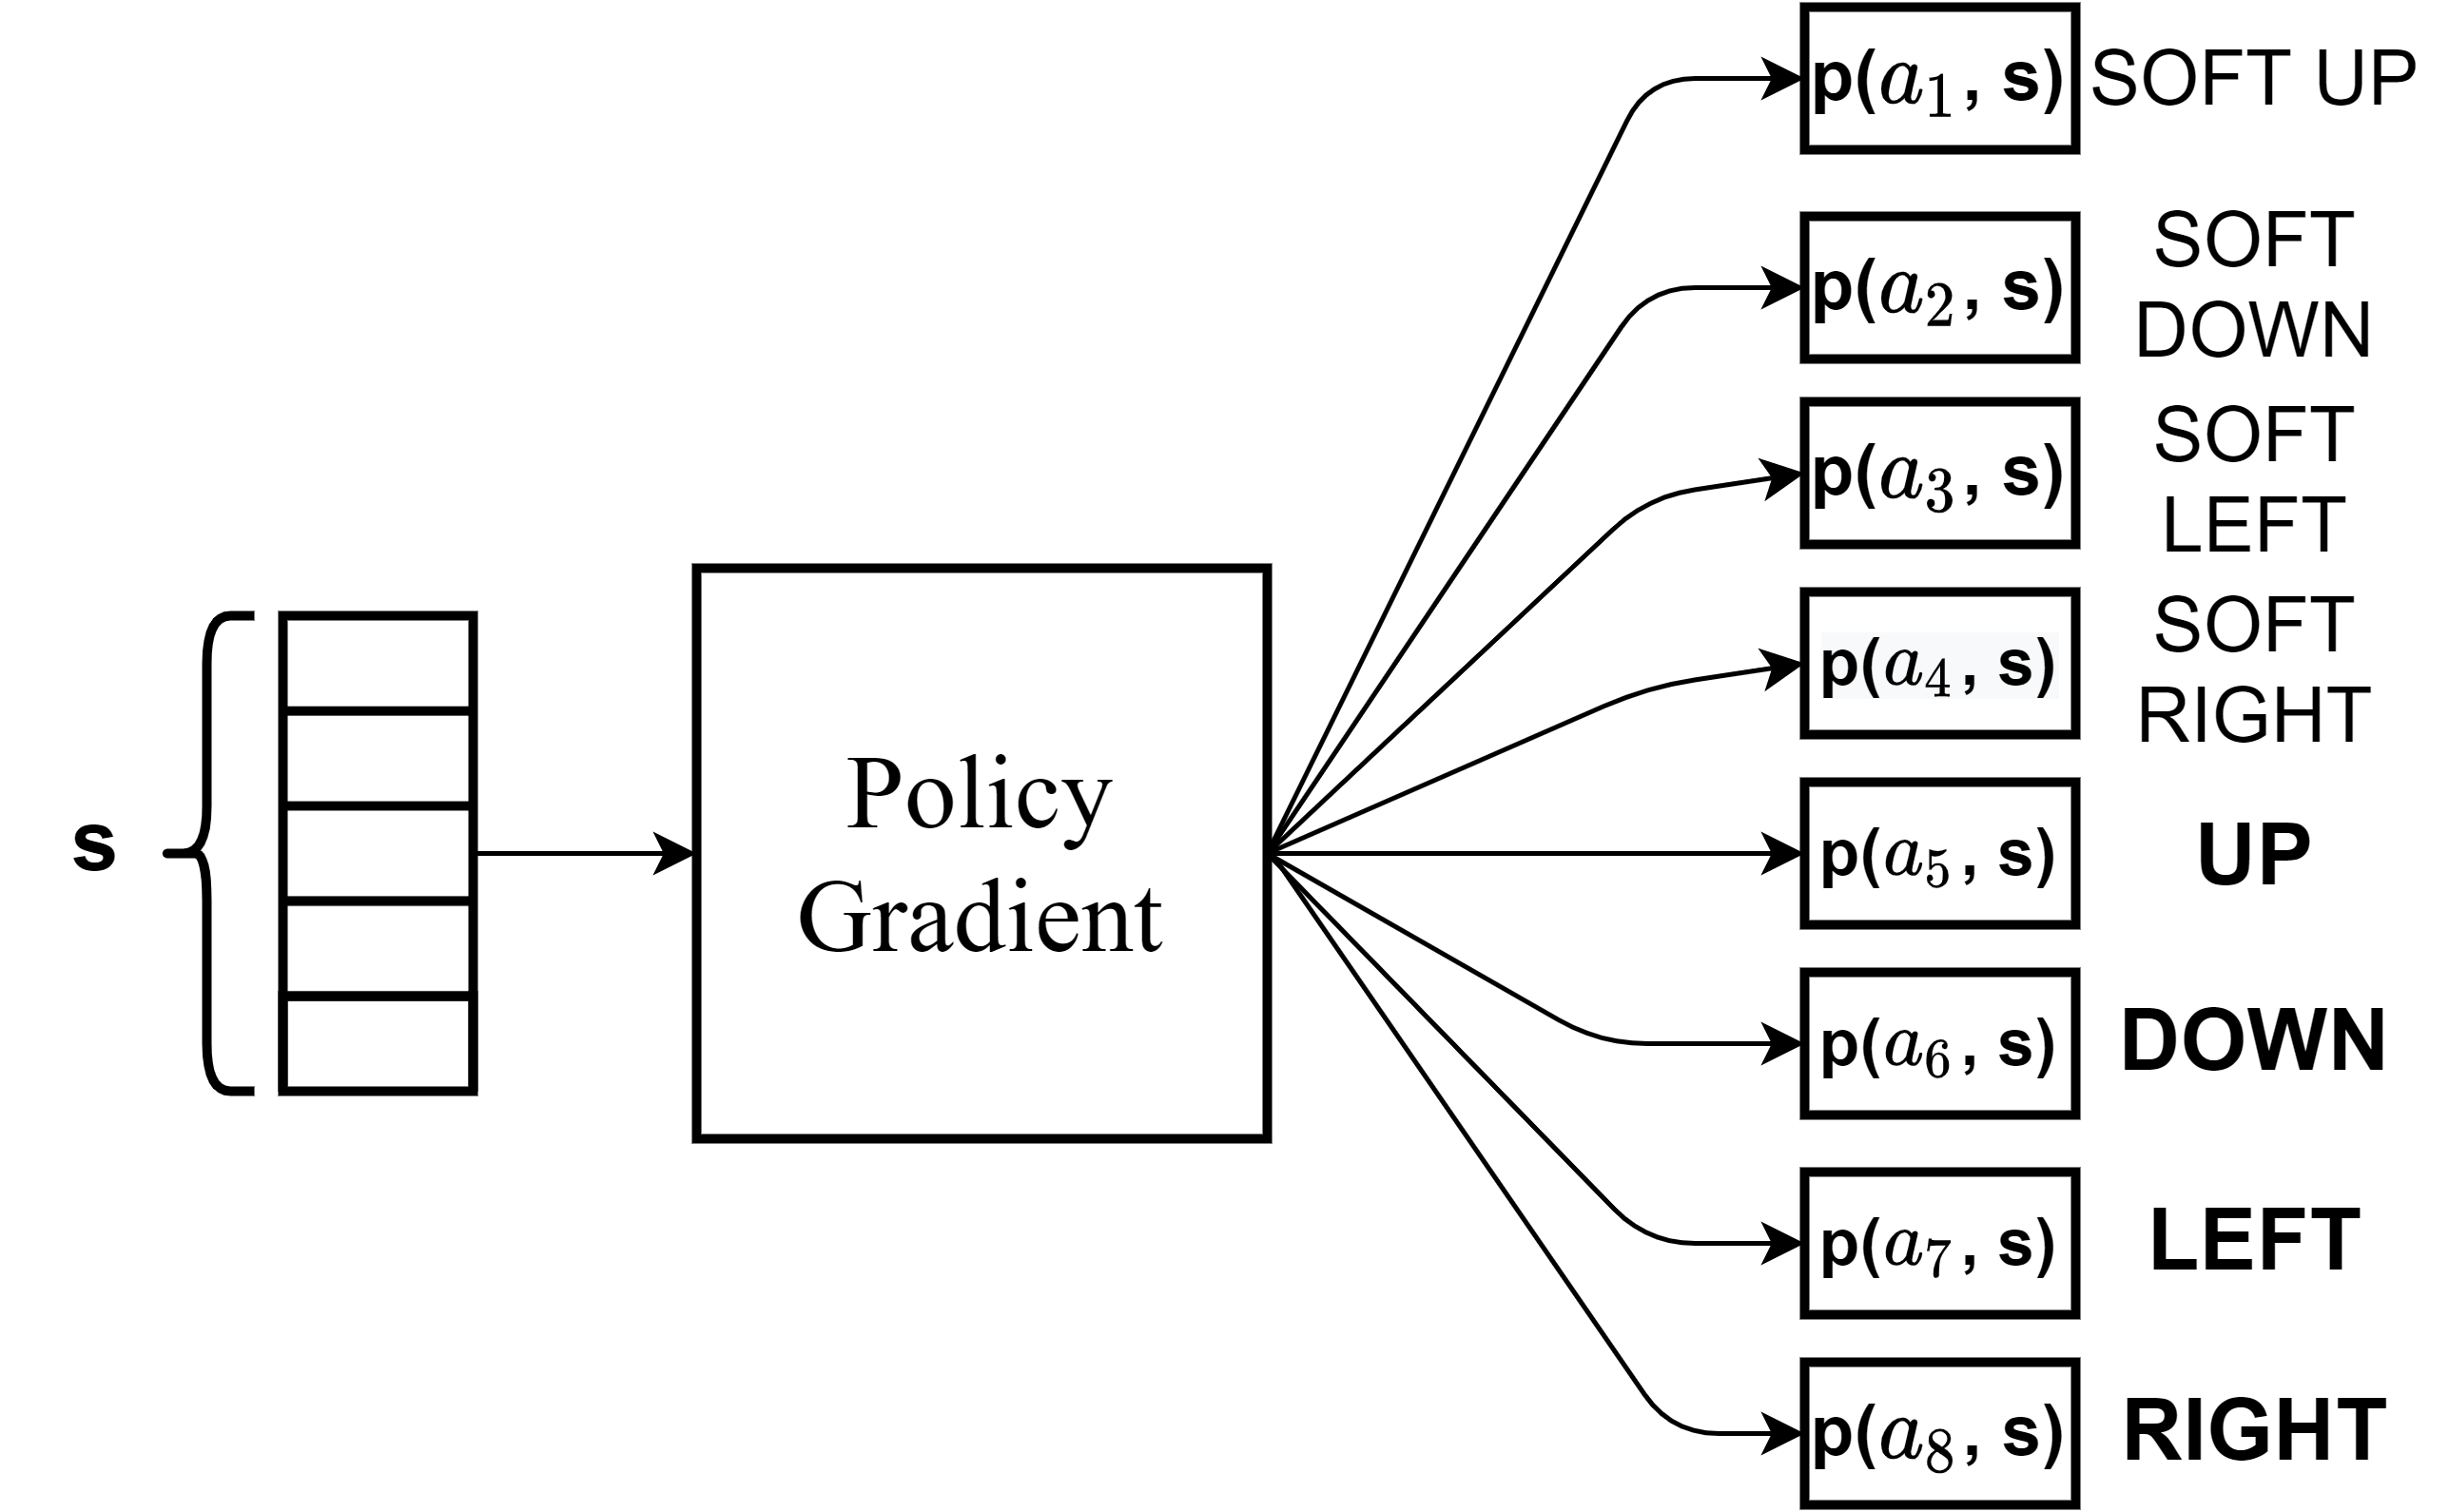
\includegraphics[width=0.6\textwidth]{Figures/Ch_RL/PG.png}
    \caption{Policy Gradient implementation}
    \label{fig:RL_PG}
\end{figure}
\subsubsection{Exploration \& Exploitation}
\label{subsec:RL_PG_exploration_n_exploitation}

In contrast to QL/DQN, PG trains a stochastic policy, where the actions are sampled based on the probability associated with selecting any action ($p(s|a)$). The amount of randomness in action selection depends on the probability distribution over the action space. If the probability distribution favors one particular action (high $p(a|s)$ value) in a given state, the chances of exploration decreases in that state. On the other hand, if two actions have comparable conditional probability (as seen in  Figure \ref{fig:RL_PG}), this will imply that the agent is not very confident in its action selection and should explore between the two high probability actions. This is in contrast with QL, where only the action associated with the highest probability was chosen and the rest were treated the same and explored based on the value of the parameter `$\epsilon$'.

An example of the same is shown in Figure \ref{fig:A2C_is_probabilistic} (a), where the Q-Learning algorithm will always choose the action associated with label two (2) based on the greedy policy. On the other hand, A2C will sample all the actions based on the probability associated with each action in Figure \ref{fig:A2C_is_probabilistic} (b). 
\begin{figure}[h!]
    \centering
    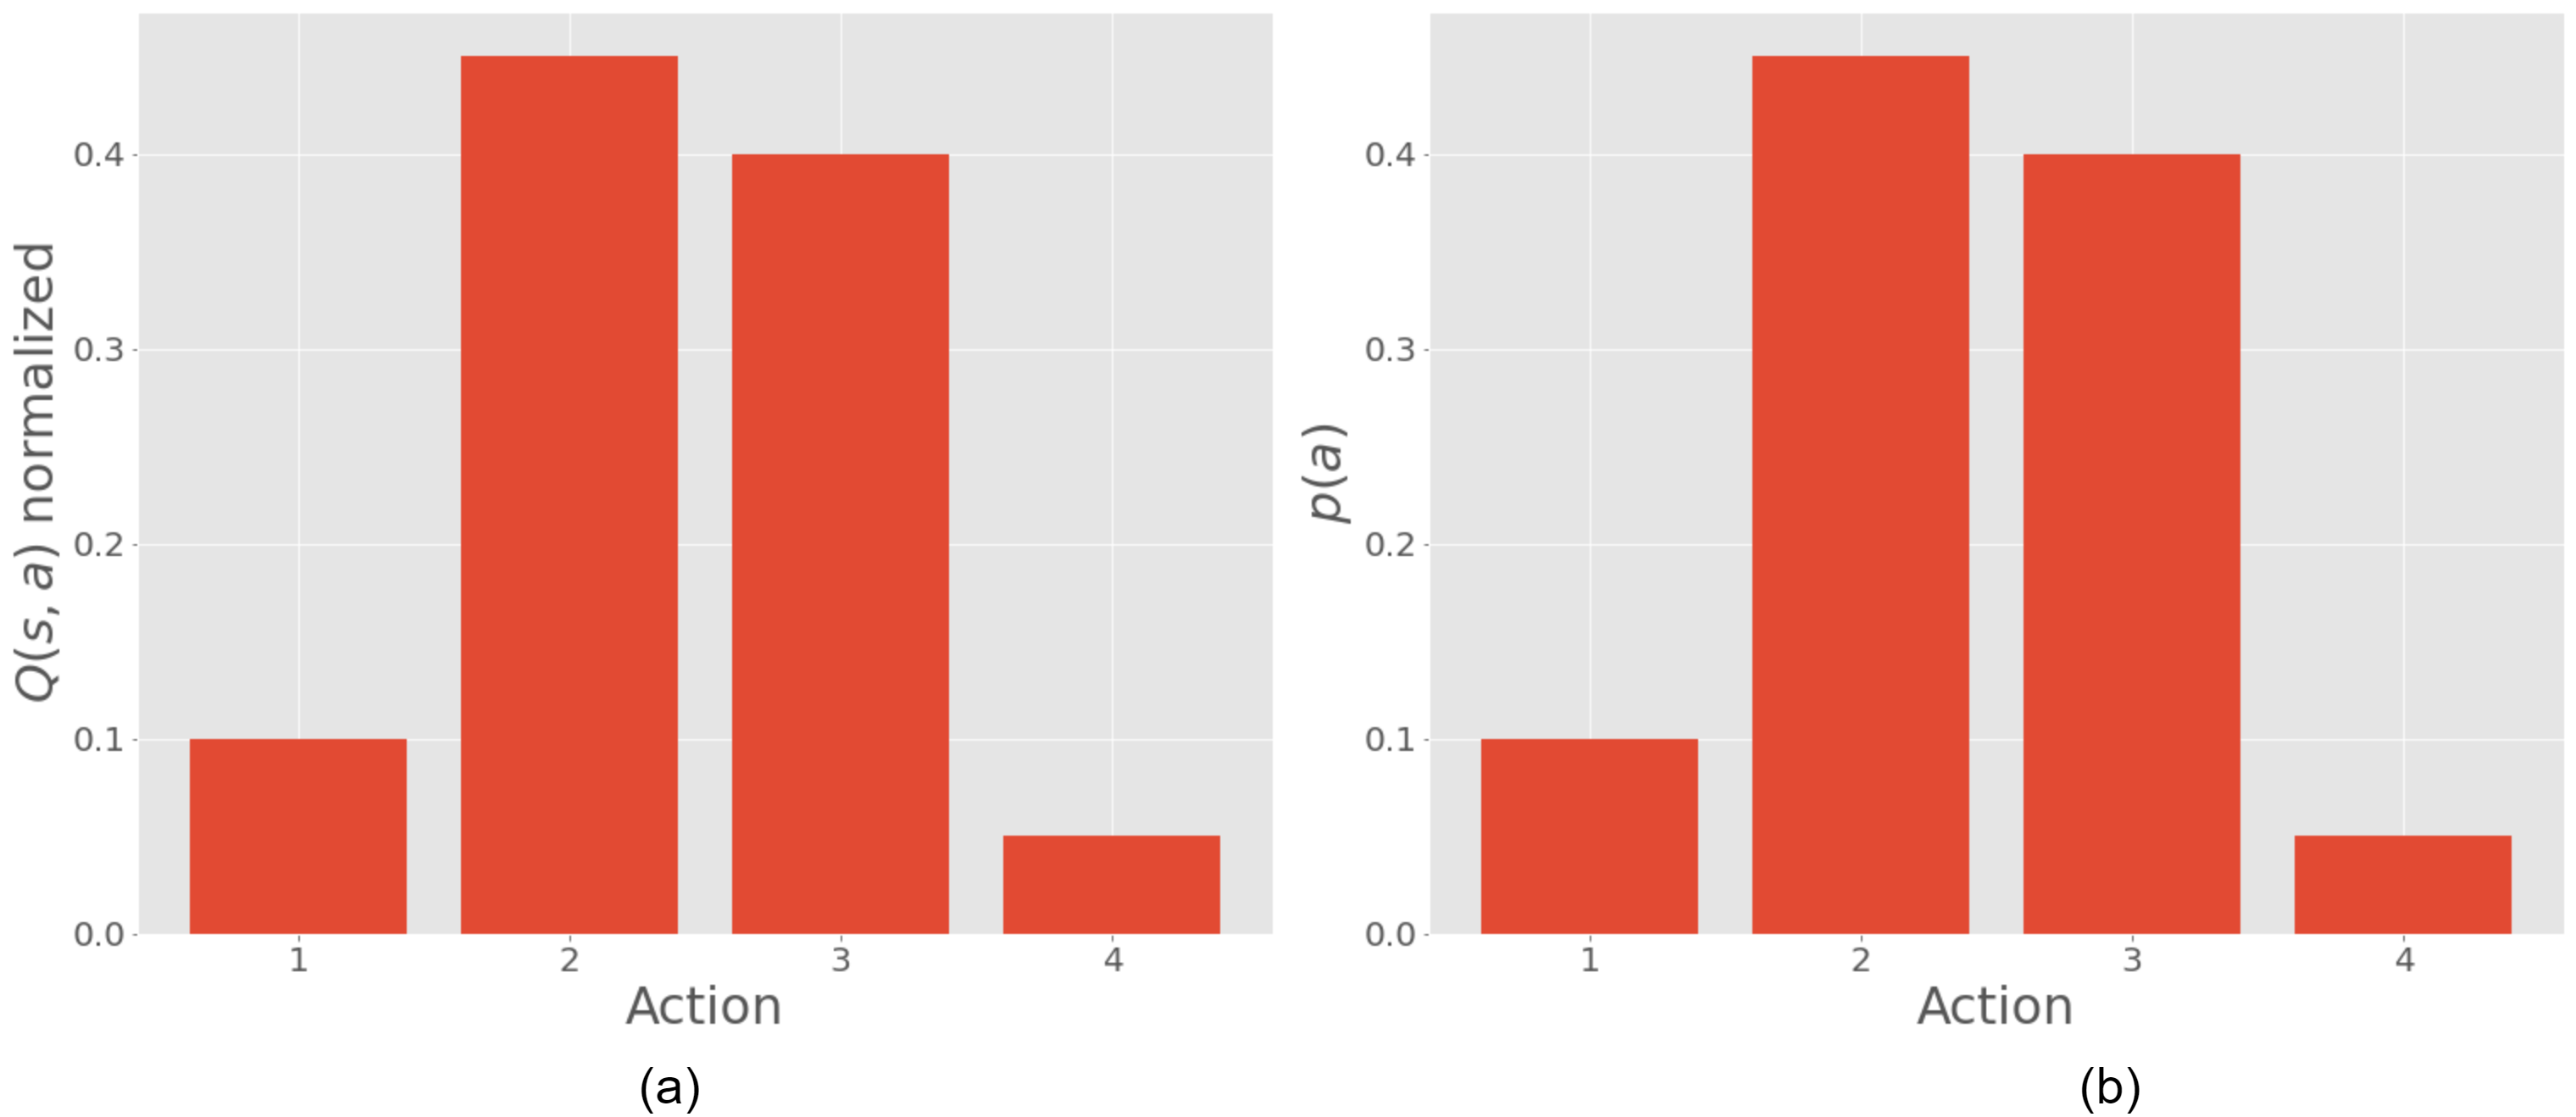
\includegraphics[width=\textwidth]{Figures/Ch_RL/A2C_vs_QL.png}
    \caption{(a) Greedy QL policy always chooses action:2, (b) Probabilistic policy with A2C samples all actions}
    \label{fig:A2C_is_probabilistic}
\end{figure}

As such action labels 2 \& 3, having comparatively high conditional probability will be sampled more as the optimal action in the given state ($s$). Additionally, there will still be some instances where the rest of the actions (1 \& 4) will be sampled. Overall, the probability of occurrence of any of the possibilities from the action space is not zero as was the case with QL.

\subsection{Improvement to Policy Gradient}

Unlike Q-learning, the PG algorithm is an on-policy algorithm, which means it learns only using state-action transitions made by the current active policy. Technically, this means there is no `Experience Replay' memory as in DQN. Once the model is trained, its parameters ($\theta$) change, and therefore its policy. This means that all the experience collected before this training must be discarded, and cannot be used for training at any later stage. So every piece of data collected for training is used only once.

\subsubsection{Actor Critic}
For PG, agents were designed to learn a policy directly and are trained based on a performance metric, which is to be maximized. As such the chances of selecting an action with a positive impact on the performance further increases. However, the performance metric, in this case, is the total reward expected in an episode. Getting the true value of the return ($G_t$) requires waiting for the episode to end, delaying the updates to the weights. This can be computationally expensive. In Section \ref{subsubsec:MDP_Q_learning}, similar issues led to discarding the MC algorithms. To overcome this, it will be better to merge the two techniques of RL that are discussed in this chapter: 

\begin{enumerate}
    \item The agent learns the policy directly based on the Policy Gradient (PG) method.
    \item At the same time, learning the state- or action-specific knowledge through the value functions ($Q(s, a )$ or $V(s)$).
\end{enumerate}

The combined method is known as ``Actor-Critic" (AC), and is made of two functions/networks learning together: one learns the policy which determines the behaviour /action of the agent (and is therefore known as the Actor), and the other network learns the Q-Value of each state and action pair (and is known as the Critic), where Q-value is also a learned parameter/network. This means that the whole system is divided into two parts or two sub-agents, which yields a more complex network as shown in Figure \ref{fig:RL_AC_generic}. 

\begin{figure}[h!]
    \centering
    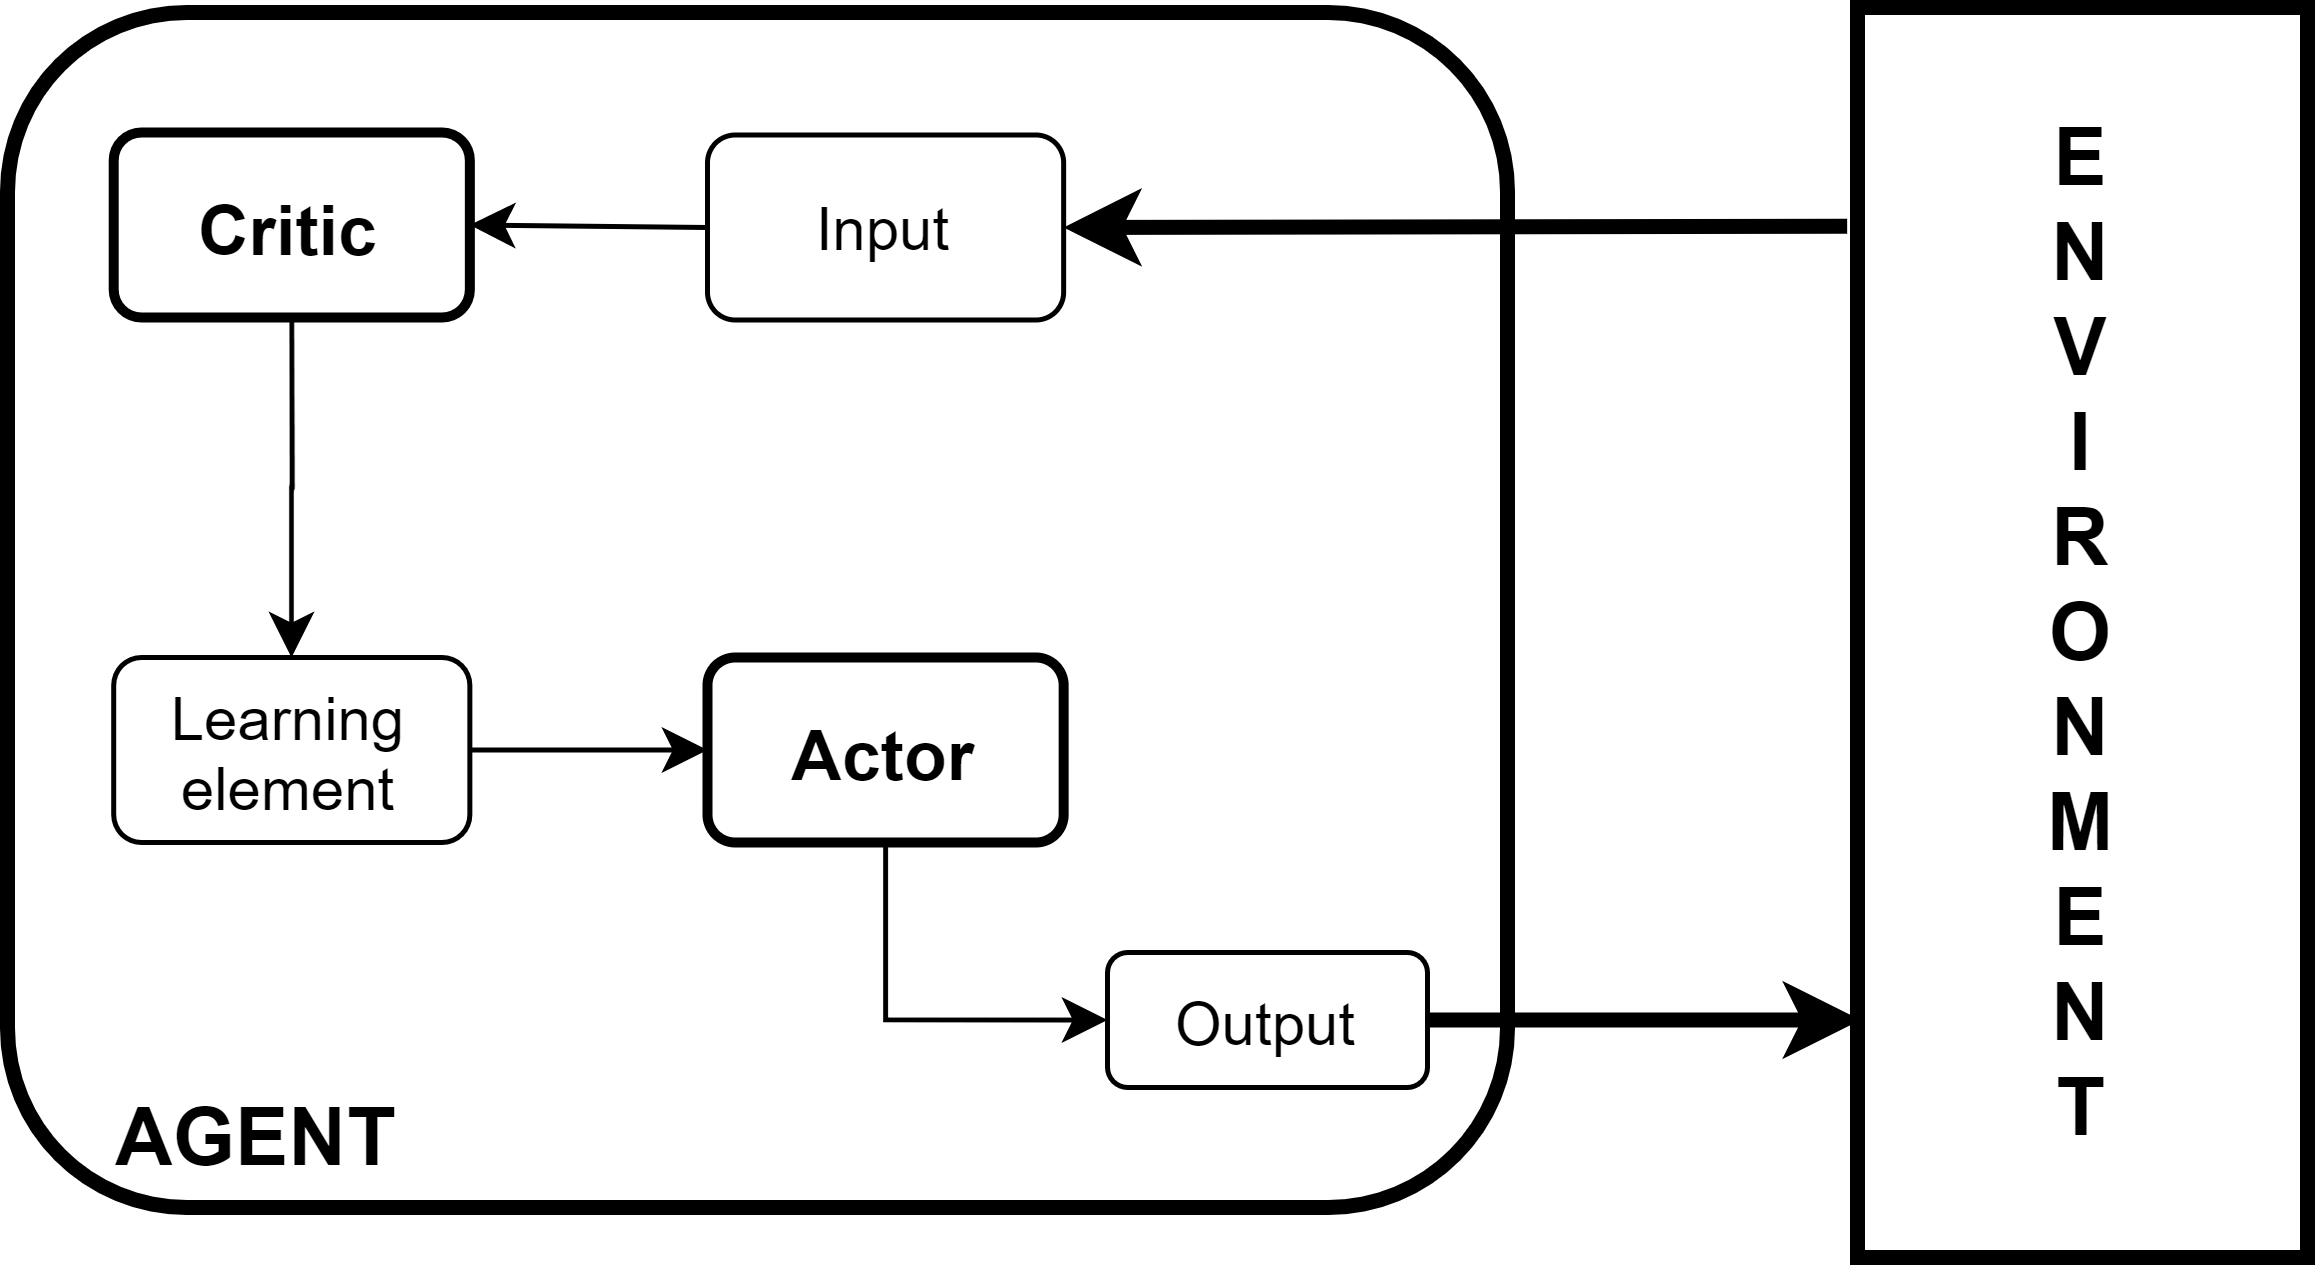
\includegraphics[width=0.65\textwidth]{Figures/Ch_RL/AC_generic.png}
    \caption{Generic AC}
    \label{fig:RL_AC_generic}
\end{figure}

A policy $\pi_{\theta}(a|s)$, defined as the probability of an agent taking action `a' in any state `s', is expressed as 
\begin{align}
    \pi_{\theta}(a|s) = \frac{e^{f(s, a, \theta)}}{\sum_{a_i} e^{f(s, a_i, \theta)}} \label{eqn:RL_A2C_probabilistic}
\end{align}
where the policy ($\pi$) has $\theta$ as its parameters and gives a probability distribution for selecting an action `$a$' over all the possible actions ($a_i$) conditioned on the current state ($s$). `$f$' is the output of the function approximator. This approach of policy parametrization is called soft-max \parencite{goodfellow2016deep} in action preferences. As mentioned earlier, the function `$f$' can be a linear combination of features or a deep neural network, as long as the policy ($\pi_{\theta}(a|s)$) is differentiable with respect to its parameters.

The update rule mentioned in eqn. \ref{eqn:RL_PG_5_13} is modified to be:

\begin{align}
    \theta_{t+1} = \theta_t + \alpha \Big(Q(s_t, a_t) \times \nabla_{\theta} \Big[ \ln \pi(a_t | s_t; \theta_t) \Big] \Big) \label{eqn:AC_update_with_Q_value}
\end{align}

where $\nabla \pi_{\theta_{t}} (a^*|s)$ is the direction in which to move $\theta_t$ so as to increase the estimate of $\pi_{\theta_{t}} (a^*|s)$ the fastest and thus increase the probability of selecting $a^*$ more often in states similar to $s$.

In the above setting, just like the PG method, AC is also an on-policy model, which means that after each training all previous data is discarded. 

\subsubsection{Advantage Actor Critic}
A further extension to AC algorithms is to replace the Q-value (in eqn. \ref{eqn:AC_update_with_Q_value}) with another performance metric called `Advantage'. This is because an absolute value of $Q(s,a)$ is extremely dependent on the reward function and can be noisy during the initial stage. Further, an incorrect initialization of $Q(s,a)$ values should not have a significant effect on the update rule as a very high and noisy value of $Q(s,a)$ can disturb the update rule in a significant way. For this, it is important to quantify the value of the $Q$-function and a comparison with the other actions is a far better representative of how good certain action is. This is represented as `advantage', i.e.\ the advantage of taking a particular action `$a$', in comparison to other actions $a \in \mathdc{A}$. So we can replace the $Q$-Value in the Actor-Critic update rule (eqn. \ref{eqn:AC_update_with_Q_value}) with the `advantage' of an action ($A(s, a)$), which is defined by subtracting $V(s)$ from $Q(s,a)$. This function gives an indication to the agent as to how much better or worse taking action `$a$' in a state `$s$' is compared to acting according to the policy \parencite{mnih2016asynchronous}. 

\begin{align}
    A(s, a) = Q(s,a) - V(s) \label{eqn:AC_Advantage}
\end{align}

where $V(s)$ is the state’s Value function (refer to Section \ref{section:MDP_QL-Value_Function}). An update to the weights ($\theta$) with $A(s,a)$ is comparatively much more useful for the gradient calculation than $Q(s,a)$, as a positive $A(s,a)$ is good (an improvement over the current policy), and a negative $A(s,a)$ is relatively bad as compared to the action suggested by the current policy. This developed form of the Actor-Critic model is known as the Advantage Actor-Critic, which is abbreviated to A2C \parencite{mnih2016asynchronous}, as shown in Figure \ref{fig:RL_A2C}.

\begin{comment}
we “push” harder on the actions that have a higher Q value, and subtracting any value that doesn’t depend on the action will preserve the ranking of how hard we push on the various actions.
\textit{In fact, it is widely recommended for the reasons described above and also because it is supposed to reduce the variance of the gradient updates.} [Citation]
\end{comment}

Based on eqn. \ref{eqn:AC_Advantage}, it might seem that the A2C version seems to make learning a little more complex, as the learning system needs to learn both $Q(s,a)$ and $V(s)$. However, that is not needed since a Q-Value is the reward received from state ($s$) and action ($a$) and then continue following the greedy policy till the end of the episode and can be written as:

\begin{align}
    Q(s,a) = r(s,a) + \gamma V(s')
\end{align}

which means that a $Q$-value is the sum of the immediate reward and the state value ($V$) of the next state ($s^'$). This results in the following equation for the `Advantage' function ($A(s,a)$):

\begin{align}
    A(s,a) = \Big( r(s,a) + \gamma V(s') \Big) - V(s)
\end{align}

This means that an agent needs to learn only the State-Value Function, and use it twice - Once for the present state ($s$) and then for the next state ($s^’$). This little tweak makes the A2C easier to implement than the original Actor-Critic.

\begin{figure}[h!]
    \centering
    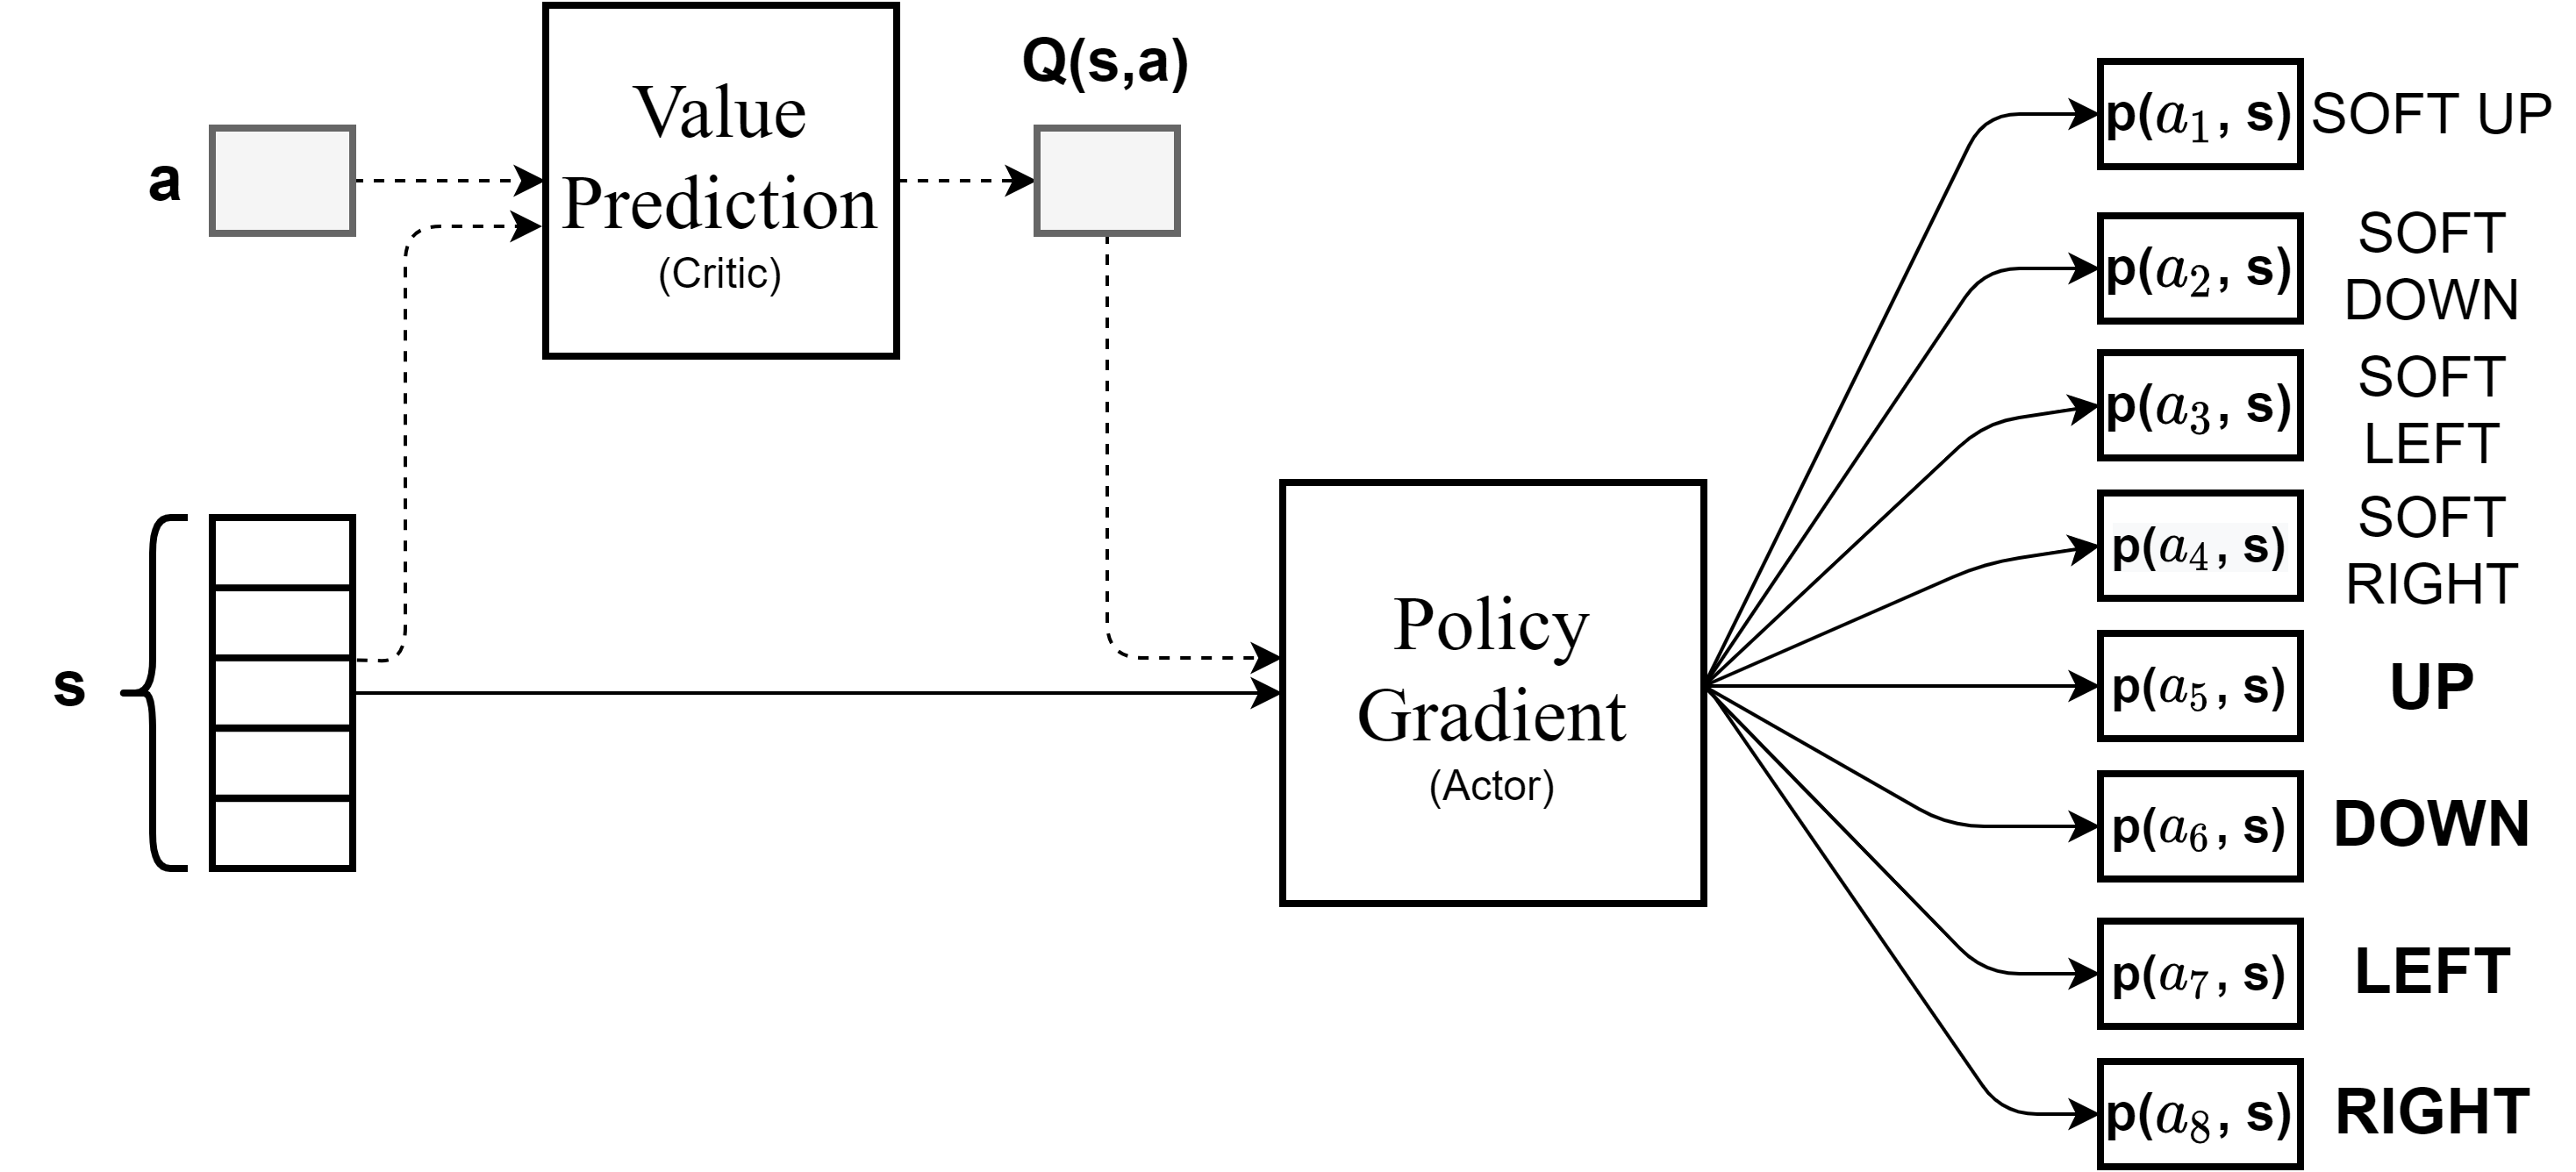
\includegraphics[width=\textwidth]{Figures/Ch_RL/AC.png}
    \caption{Advantage Actor Critic}
    \label{fig:RL_A2C}
\end{figure}

\begin{comment}

Poor performance over a large set of actions.
Actions set must be finite.
Poor exploration strategy.
\end{comment}

\section{Experiment Setup - A2C}

As shown in Figure \ref{fig:RL_network_architecture_Ccore}, the network architecture takes in the state representation and outputs the probability distribution over the possible eight actions available to the agent at any given time (based on \textit{SeqTO-v2}). A few cases with varying coil turns and coil current are considered. For testing the generalizability of the A2C algorithm, it is trained on only three out of the possible eight excitation scenarios for a C-core, as listed in Table \ref{tab:RL_scenario_c_core}.

\begin{figure}[h!]
    \centering
    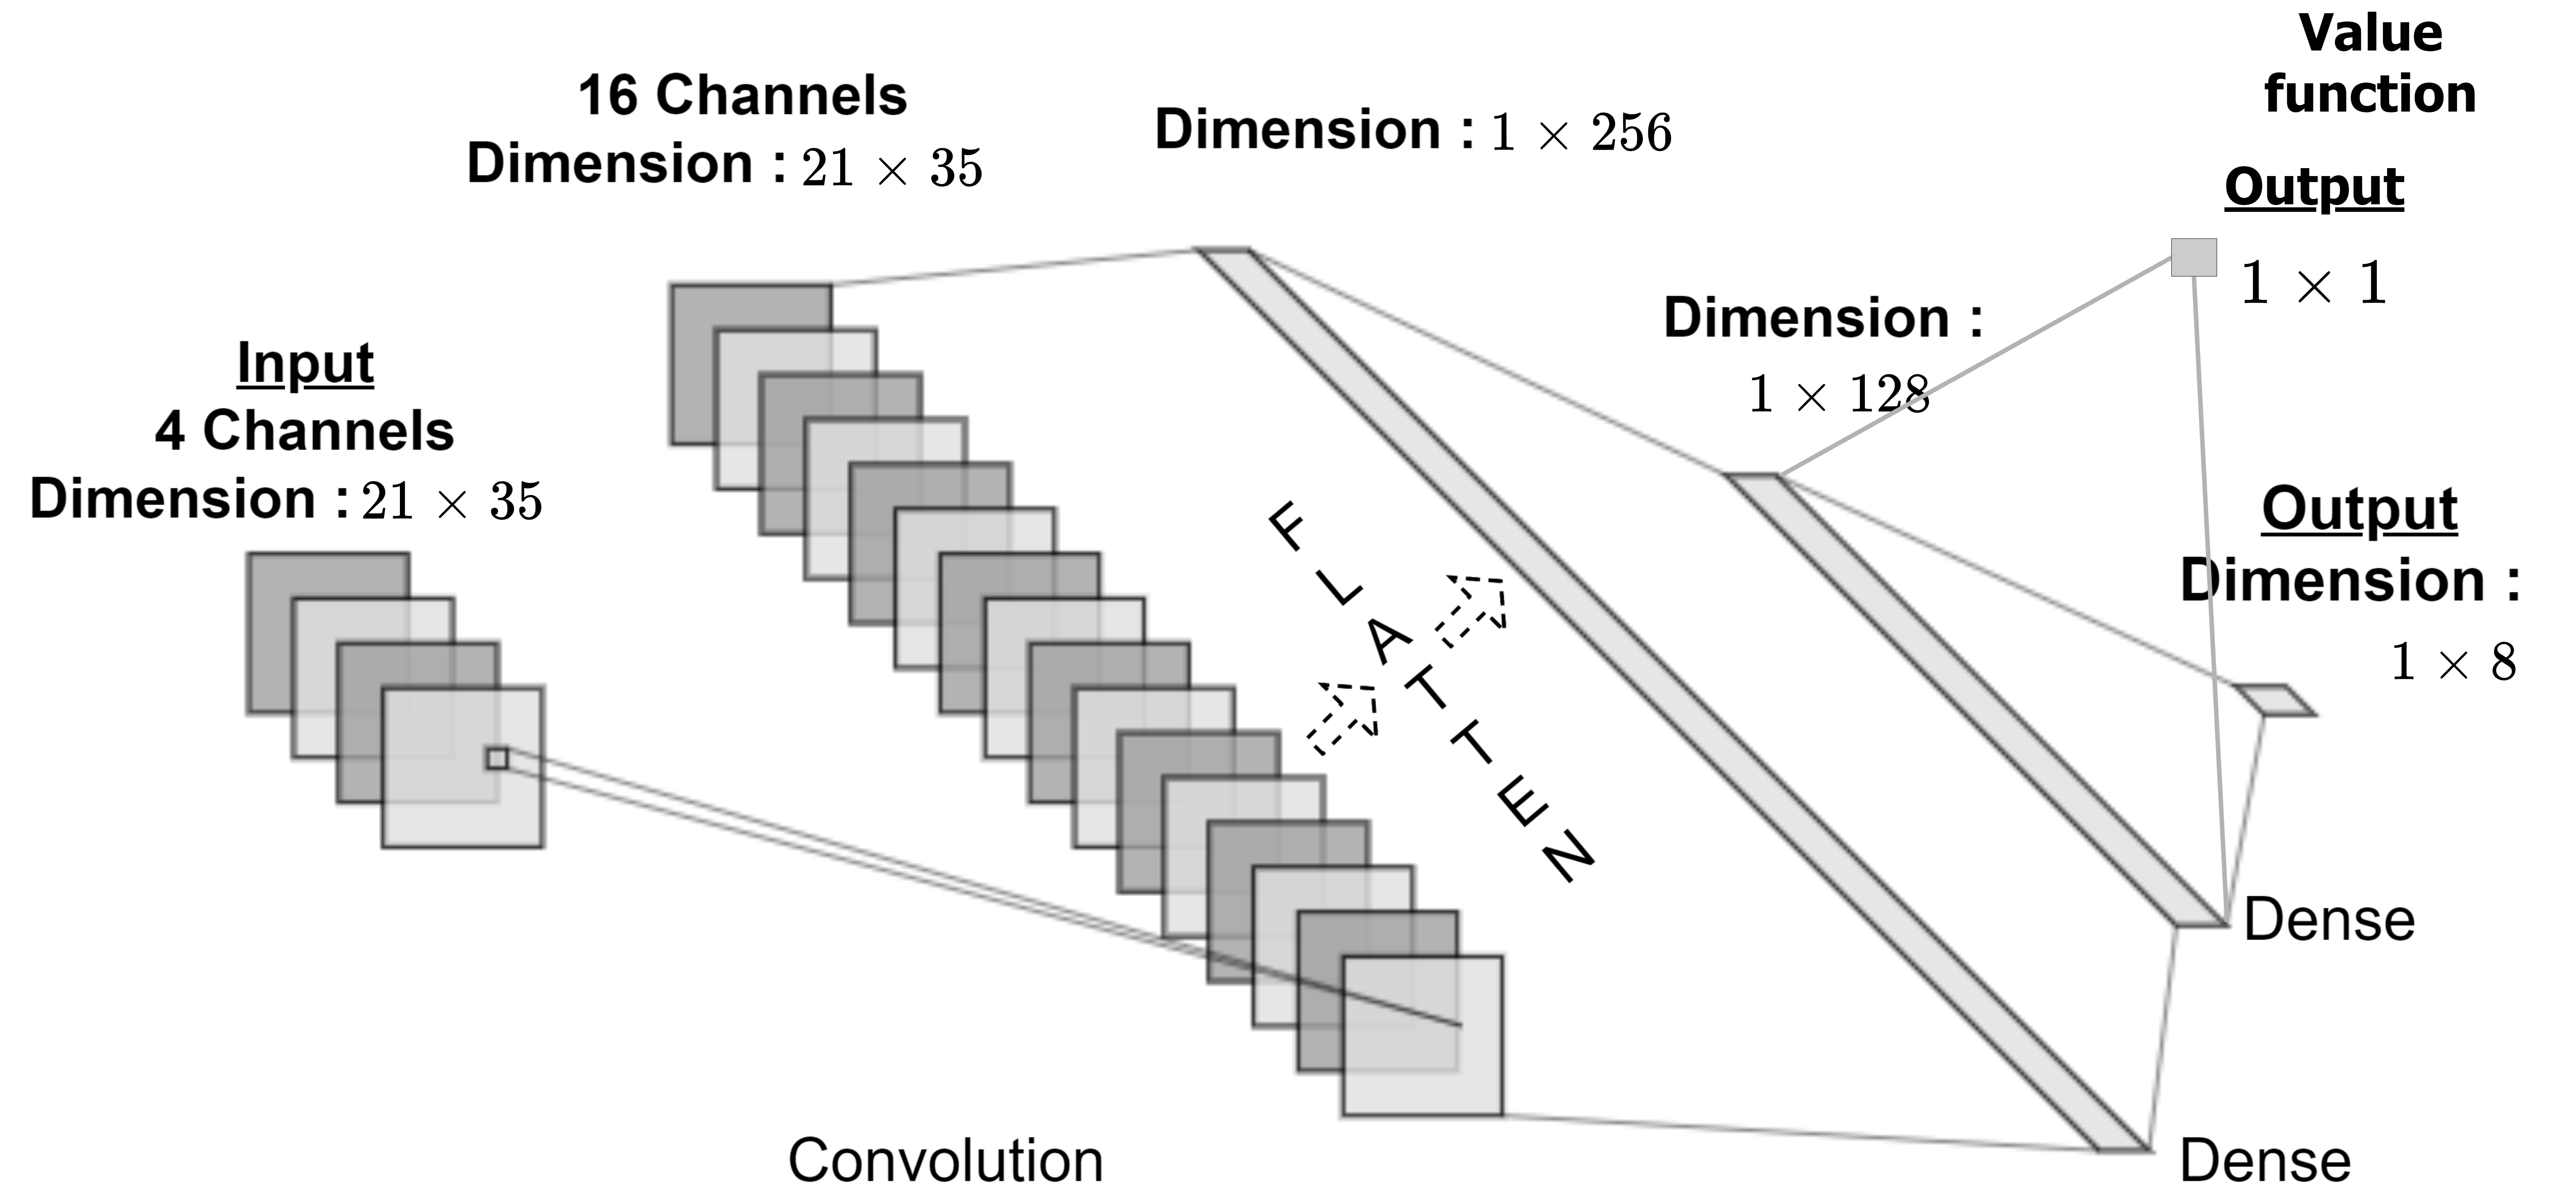
\includegraphics[width=\textwidth]{Figures/Ch_RL/nn_intelligent_agent6.PNG}
    \caption{Network Architecture for A2C}
    \label{fig:RL_network_architecture_Ccore}
\end{figure}

\usepackage{}
\begin{table}[h!]
\centering
\begin{tabular}{|c|c|c|c|}
\hline
\textbf{Type} & \textbf{Scenario} & \textbf{\begin{tabular}[c]{@{}c@{}}Coil current\\ (A)\end{tabular}} & \textbf{\begin{tabular}[c]{@{}c@{}}No. of turns\\ (T)\end{tabular}} \\ \hline \hline
\multirow{3}{*}[-0.2em]{\begin{sideways}TRAIN\end{sideways}} & 1. & 1.0 & 250 \\ \cline{2-4} 
& 2. & 1.0 & 500 \\ \cline{2-4} 
& 3. & 1.5 & 500 \\ \hline \hline
\multirow{3}{*}[-1.5em]{\begin{sideways}TEST\end{sideways}} & 4. & 0.5 & 250 \\ \cline{2-4} 
& 5. & 0.75 & 500 \\ \cline{2-4} 
& 6. & 1.25 & 500 \\ \cline{2-4} 
& 7. & 1.75 & 500 \\ \cline{2-4} 
& 8. & 2.0 & 500 \\ \hline
\end{tabular}
\caption{Different excitation scenarios used for TO of a C-core actuator.}
\label{tab:RL_scenario_c_core}
\end{table}

\begin{figure}[h!]
    \centering
    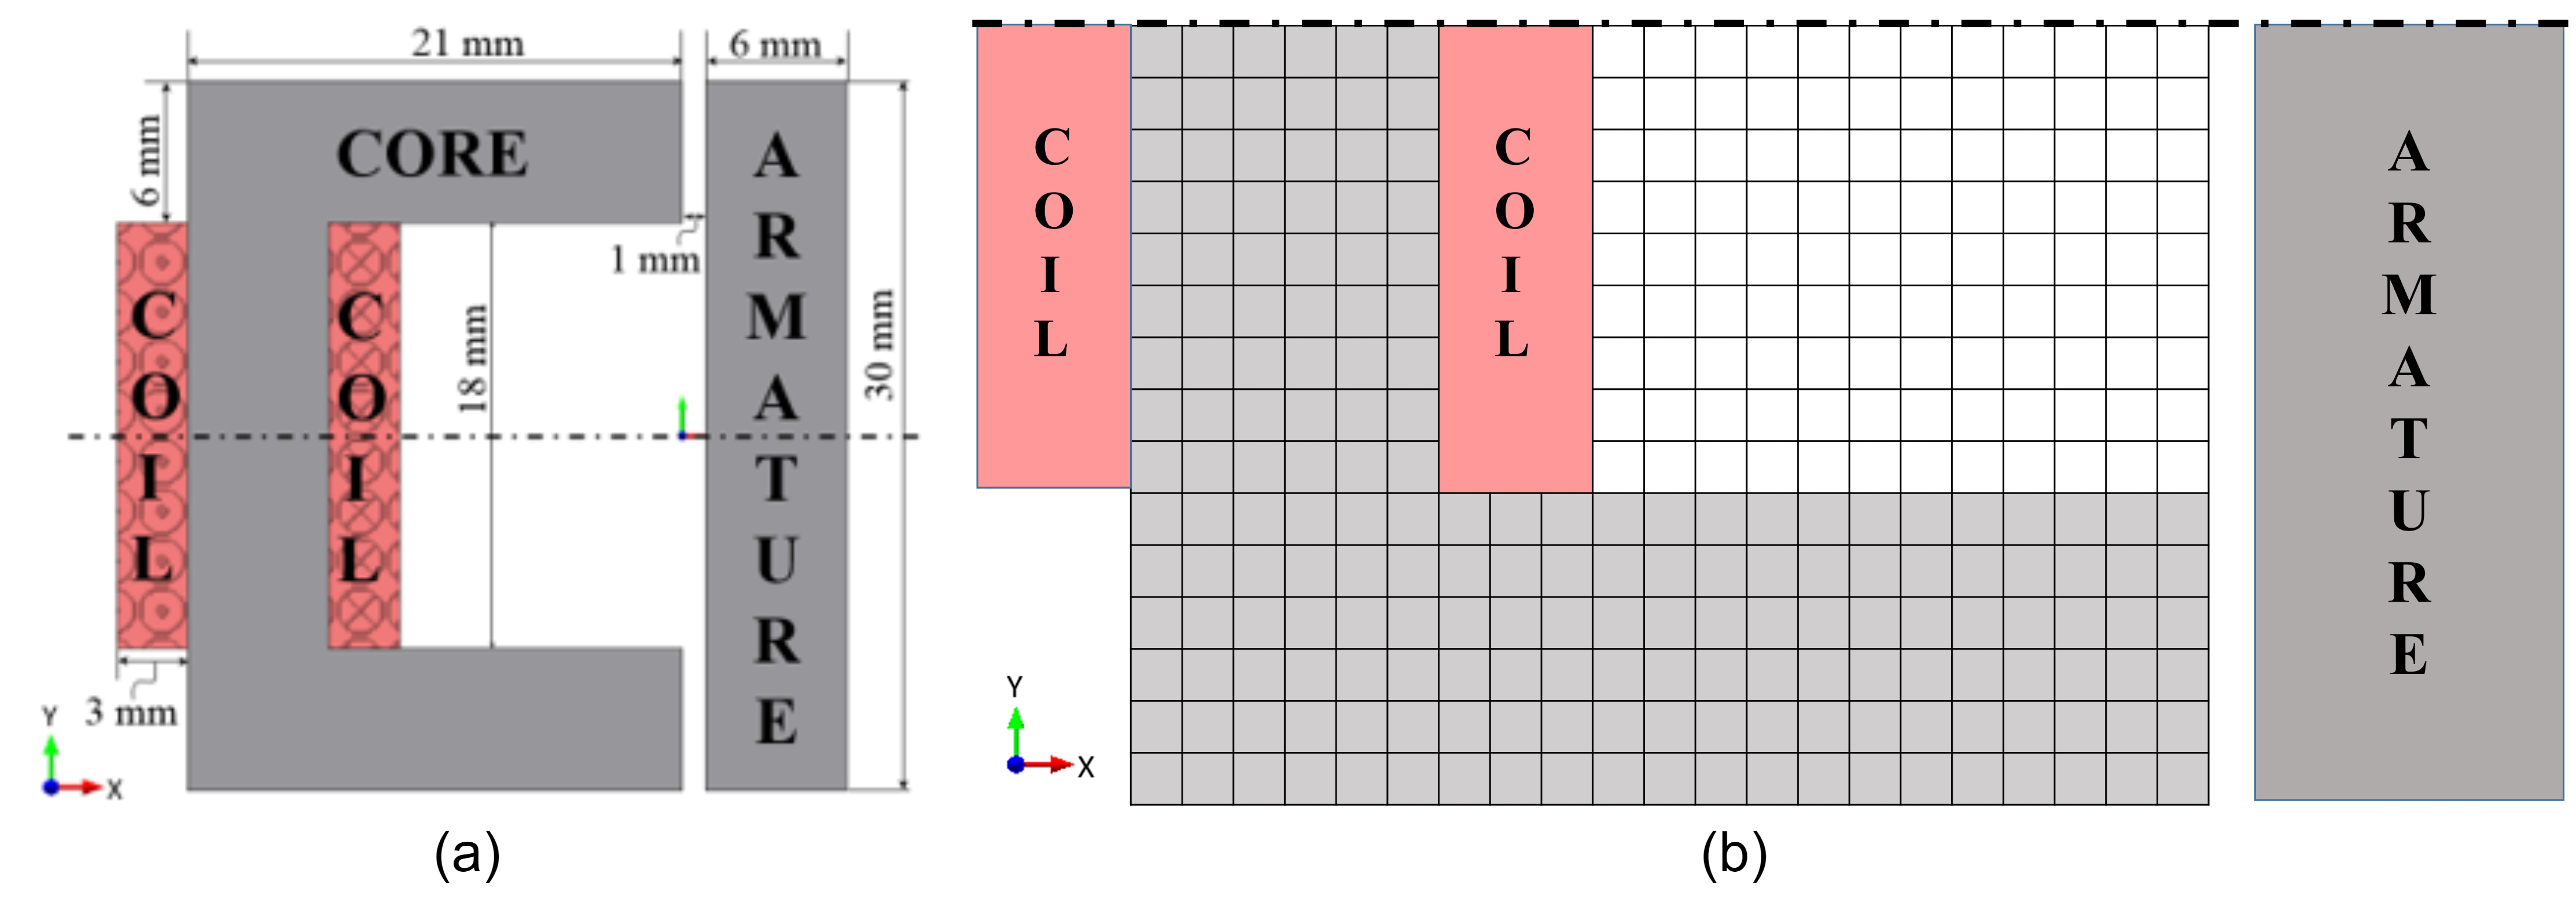
\includegraphics[width=0.85\textwidth]{Figures/Ch_RL/c_core_conventional_latex.png}
    \caption{(a) Conventional C-core design (b) Only half of the geometry is simulated due to symmetricity.}
    \label{fig:RL_c_core_conventional_latex}
\end{figure}

The scenarios where the agent interacts, collects, and train on data originating from the scenario, is labeled as `\textit{Train}’. The rest of the scenarios are used to check the `generalizability' of the agent and are referred to as the `\textit{Test}’ scenarios. After every few iterations of training, the agent is tested on all the scenarios listed in Table \ref{tab:RL_scenario_c_core} to check the performance and monitor if the agent converged to a solution. The optimal design obtained from A2C is compared with that obtained using GA \parencite{park2009magnetic, midha2019selection}. The GA algorithm operates on the On-Off TO methodology. Further, a tabular Q-Learning method is also employed with SeqTO-v1 (pointer size $1 \times 1$) to verify the results. The comparison is performed on the value of the performance parameter (force on the armature in C-core) of the optimal design obtained through each method. The value of the torque is also compared with the conventional design of a C-core. The geometry shown is Figure \ref{fig:RL_c_core_conventional_latex} is considered as the conventional geometry of the C-core for this study. In addition, a comparison of the number of simulation calls made for each optimization process is also tabulated. 

The network used for Actor \& Critic is shown in Figure \ref{fig:RL_network_architecture_Ccore}. The network starts with a convolutional layer to capture the spatial relationship of the material distribution in the design domain and the corresponding material distribution for the current and past 4 states. This is followed by two dense layers and an output layer which correspond to the $Q(s,a)$ for the critic and $\pi(s,a)$ for the Actor network. Apart from the output layer, which is dense (used for regression) for Critic and Softmax (used for distinct classes) for the Actor, the rest of the network architecture and functionality remains the same and can thus be merged to form a single input multi-output network as can be seen in Figure \ref{fig:RL_network_architecture_Ccore}.

After the training, it is observed that the A2C based agent managed to produce a superior performance on the excitation cases which are part of `\textit{training}' scenarios as compared to the performance on the `\textit{test}' scenarios. However, the performance over the `test' cases can be further improved by using the technique of transfer learning (TL). Some of the same concepts of TL as discussed in Chapter \ref{chapter:3_RNN} and \parencite{khan_transfer} can be used here. During the fine-tuning/ re-training, the learning rate is reduced but the network architecture is not altered as the design domain and the MDP encoding was kept the same.

\section{Results \& Discussion}

The results obtained over the scenario cases for different excitation for the C-core are tabulated in Table \ref{tab:PG_results}. This shows a comparison over computational efficiency and optimal accuracy of all RL based algorithms using Sequence-based TO (-v1 \& -v2) with that obtained from GA \parencite{park2009magnetic} and GA + filters \parencite{midha2019selection} using ON/OFF TO. The performance improvement can be observed in all five cases, where the previous results from \cite{midha2019selection} were available. Some additional scenarios are analyzed for which results from the original work \parencite{midha_2018} were not available, specifically (\textit{1.25 A, 500 Turns}), (\textit{1.75 A, 500 Turns}) \& \textit{2.0 A, 500 Turns}). 
This is performed as part of the inference check of the neural network-based A2C algorithms.

% Please add the following required packages to your document preamble:
% \usepackage{graphicx}
\begin{table}[h!]
\centering
\resizebox{0.99\textwidth}{!}{%
\begin{tabular}{|c|c|c|c:c|c|c:c|}
\hline
\textbf{}   
& \textbf{Scenario}   
& \textbf{\begin{tabular}[c]{@{}c@{}}Conven \\ -tional\end{tabular}}
& \textbf{\begin{tabular}[c]{@{}c@{}}GA\\ On/Off \\ {\tiny (\citeauthor*{park2009magnetic})}\end{tabular}}
& \textbf{\begin{tabular}[c]{@{}c@{}}+Filter\\ {\tiny (\citeauthor{midha2019selection})}\end{tabular}}
& \textbf{\begin{tabular}[c]{@{}c@{}}QL\\ SeqTO \\ ($1 \times 1$)\end{tabular}}
& \textbf{\begin{tabular}[c]{@{}c@{}}A2C\\ SeqTO \\ -v2\end{tabular}}
& \textbf{\begin{tabular}[c]{@{}c@{}}A2C\\ (Re-train)\end{tabular}}
\\ 
\hline \hline

\multirow{3}{*}[-1.5em]{\begin{sideways}TRAIN\end{sideways}} 
& \begin{tabular}[c]{@{}c@{}}1.0 A,\\ 250T\end{tabular}  & 9.97     
& \begin{tabular}[c]{@{}c@{}}16.80 \\ {\small(200k)}\end{tabular}    & 15.90  
& \begin{tabular}[c]{@{}c@{}}\textbf{19.02} \\ {\small(125k)}\end{tabular} 
& \begin{tabular}[c]{@{}c@{}}16.6 \\ {\small(190k)}\end{tabular} & -  
                                \\ \cline{2-8} 
& \begin{tabular}[c]{@{}c@{}}1.0A,\\ 500T\end{tabular}  & 38.70    
& \begin{tabular}[c]{@{}c@{}}50.90 \\ {\small(210k)}\end{tabular}    & 50.60
& \begin{tabular}[c]{@{}c@{}}\textbf{54.0 }\\ {\small(128k)}\end{tabular} 
& \begin{tabular}[c]{@{}c@{}}51.50 \\ {\small(150k)}\end{tabular} & -  
                                 \\ \cline{2-8} 
& \begin{tabular}[c]{@{}c@{}}1.5A,\\ 500T\end{tabular}  & 78.40    
& \begin{tabular}[c]{@{}c@{}}82.10 \\ {\small(195k)}\end{tabular}    & 83.30
& \begin{tabular}[c]{@{}c@{}}82.20 \\ {\small(105k)}\end{tabular} 
& \begin{tabular}[c]{@{}c@{}}\textbf{85.70 }\\ {\small(125k)}\end{tabular} & -  
                                \\ \hline \hline
\multirow{3}{*}[-4em]{\begin{sideways}TEST\end{sideways}} 
& \begin{tabular}[c]{@{}c@{}}0.5A,\\ 250T\end{tabular}  & 2.52     
& \begin{tabular}[c]{@{}c@{}}4.56 \\ {\small(159k)}\end{tabular}    & 3.88
& \begin{tabular}[c]{@{}c@{}}\textbf{4.93} \\ {\small(94k)}\end{tabular} 
& \begin{tabular}[c]{@{}c@{}}4.75 \\ {\small(175k)}\end{tabular} 
& \begin{tabular}[c]{@{}c@{}}4.91 \\ {\small(3500)}\end{tabular}
                                \\ \cline{2-8} 
& \begin{tabular}[c]{@{}c@{}}0.75A,\\ 500T\end{tabular} & 22.20    
& \begin{tabular}[c]{@{}c@{}}32.50 \\ {\small(160k)}\end{tabular}    & 30.80
& \begin{tabular}[c]{@{}c@{}}\textbf{34.80} \\ {\small(120k)}\end{tabular} 
& \begin{tabular}[c]{@{}c@{}}32.70 \\ {\small(175k)}\end{tabular} 
& \begin{tabular}[c]{@{}c@{}}34.60 \\ {\small(7500)}\end{tabular}
                                \\ \cline{2-8} 
& \begin{tabular}[c]{@{}c@{}}1.25A,\\ 500T\end{tabular}  & 58.4    
& - & -
& \begin{tabular}[c]{@{}c@{}}71.30 \\ {\small(108k)}\end{tabular} 
& \begin{tabular}[c]{@{}c@{}}71.60 \\ {\small(150)}\end{tabular} 
& \begin{tabular}[c]{@{}c@{}}72.1, \textbf{72.3 }\\ {\small(7500)}\end{tabular}     
                                   \\ \cline{2-8} 
& \begin{tabular}[c]{@{}c@{}}1.75A,\\ 500T\end{tabular}  & 93.6    
& -    & -  
& \begin{tabular}[c]{@{}c@{}}\textbf{97.20} \\ {\small(105k)}\end{tabular} 
& \begin{tabular}[c]{@{}c@{}}96.8, 93.6 \\ {\small(135k)}\end{tabular} 
& \begin{tabular}[c]{@{}c@{}}96.8 \\ {\small(2500)}\end{tabular}   
                                \\ \cline{2-8} 
& \begin{tabular}[c]{@{}c@{}}2.0A,\\ 500T\end{tabular}  & 105    
& -    & -  
& \begin{tabular}[c]{@{}c@{}}\textbf{106} \\ {\small(115k)}\end{tabular} 
& \begin{tabular}[c]{@{}c@{}}105 \\ {\small(110k)}\end{tabular} 
& \begin{tabular}[c]{@{}c@{}}\textbf{106} \\ {\small(2750)}\end{tabular}   
                                \\ \hline \hline
\multicolumn{3}{|c|}{Total Simulations}
& (925k) & -     
& (900k) & (192k)
& (24k)
\\ \hline
\multicolumn{3}{|c|}{Avg. Simulations/Scenario}
& (185k) & -     
& (112k) & (24k)
& (4,750)
\\ \hline
\end{tabular}%
}
\caption{Comparison of Force magnitude wrt GA optimized results \parencite{park2009magnetic}, GA+filters \parencite{midha2019selection}, Tabular QL (using SeqTO-v1) optimized results and with the A2C (RL based; using SeqTO-v2) agent. The number in the brackets in each cell corresponds to the number of FE calls during the particular optimization process.}
\label{tab:PG_results}
\end{table}

To keep track for convergence, the A2C algorithm is tested at a regular interval during the training phase to check the overall performance of the agent. Along with the value of force for optimal geometry, the number of FE simulations performed in each optimization run is also recorded for comparison and is included in Table \ref{tab:PG_results}. 

For each excitation scenario, the GA and QL results are independent runs where the optimization is performed from scratch. On the other hand, a single A2C based agent is employed to learn (train) from the experience generated on the three train scenarios and generalize to all the other five `test' scenarios. In such a case, the FE calls for GA and QL are to be summed up if one needs optimal geometry for all the eight scenarios mentioned, since all the runs are independent. In contrast, for A2C, the number of simulations associated with each excitation scenario is simply a milestone during a single optimization/training session. 
As such, the number of FE simulations associated with A2C agent in Table \ref{tab:PG_results} are not to be summed up, since the number represents the simulations needed for the A2C algorithm to converge to the optimal geometry for the corresponding `train' or `test' excitation scenarios. 

It is observed that GA requires the most number of FE calls out of all the algorithms tested in the study. Further, the force on armature value of the optimal geometry identified by GA is inferior to that obtained through other algorithms. The possible cause for this is explored later. In terms of FE calls, QL required the fewest function evaluation for seven out of the eight scenarios, when considered independently. 
This can be attributed to the binding nature of the SeqTO-v1 methodology and the deterministic nature of the QL algorithm. 
Finally, if the total function evaluations for all the scenarios is to be compared, A2C out performs both QL and GA, due to the nature of SeqTO-v2 methodology and the ability of the function approximator (NN) to extract useful patterns and generalize over similar scenarios. The number of FE simulations required by QL for all (eight) scenarios sums up to 900k. 
In comparison, A2C requires only a maximum of $190,000$ FE calls to converge to an optimal solution for the three train cases. On average, QL requires about $112,000$ simulations for an excitation scenario. In comparison, the average number of simulations needed for A2C is only $24, 000$ FE simulations for an excitation scenario of a C-core. 
It can be seen that A2C achieves close to optimal geometries for all the scenarios. This is compensated by the significantly fewer number of simulations needed to achieve this solution design. In cases, where only the optimal solution is to be desired, the trained agent can be used as a source domain to further fine-tune an agent for a specific scenario. The resulting design obtained after fine-tuning achieves the same force magnitude as the optimal ones, using only a small amount of computational resources.

The inability of the agent to reach the optimal structure can partially be explained due to the inflexibility of the SeqTO-v2 methodology, where the methodology does not support placing a thin strip close to the air gap, that the QL based agent can achieve with SeqTO-v1 ($1 \times 1$) environment. However, the number of FE calls needed to use SeqTO-v1 ($1 \times 1$) will be simply too much to handle as function approximators such as neural networks will require far more training data compared to a deterministic tabular look-up table.

A qualitative discussion for some of the scenarios is presented below, where a comparison of the optimal geometry along with the plot of the magnitude of magnetic flux density is also shown.

\subsubsection{C-core Excitation Scenario 1}
\label{section:RL_c_core_excitation_1A_250T}
\textit{Coil Current $= 1.0 A$  \& Coil Turns $= 250$ }

This excitation scenario is part of the `\textit{train}’ cases, where the agent interacted with the environment operating with the excitation settings of \textit{Coil Current = 1.0 A, Coil Turns = 250}, along with two other `\textit{train}' scenarios (\textit{1.0 A, 500 Turns} \& \textit{1.5 A, 500 Turns}). The force magnitude generated by the optimal design on the armature, along with the magnetic flux density distribution obtained from the GA, QL, and A2C is shown in Figure \ref{fig:RL_Ccore_0.5A_GeoNB}. 

\begin{figure}[h!]
    \centering
    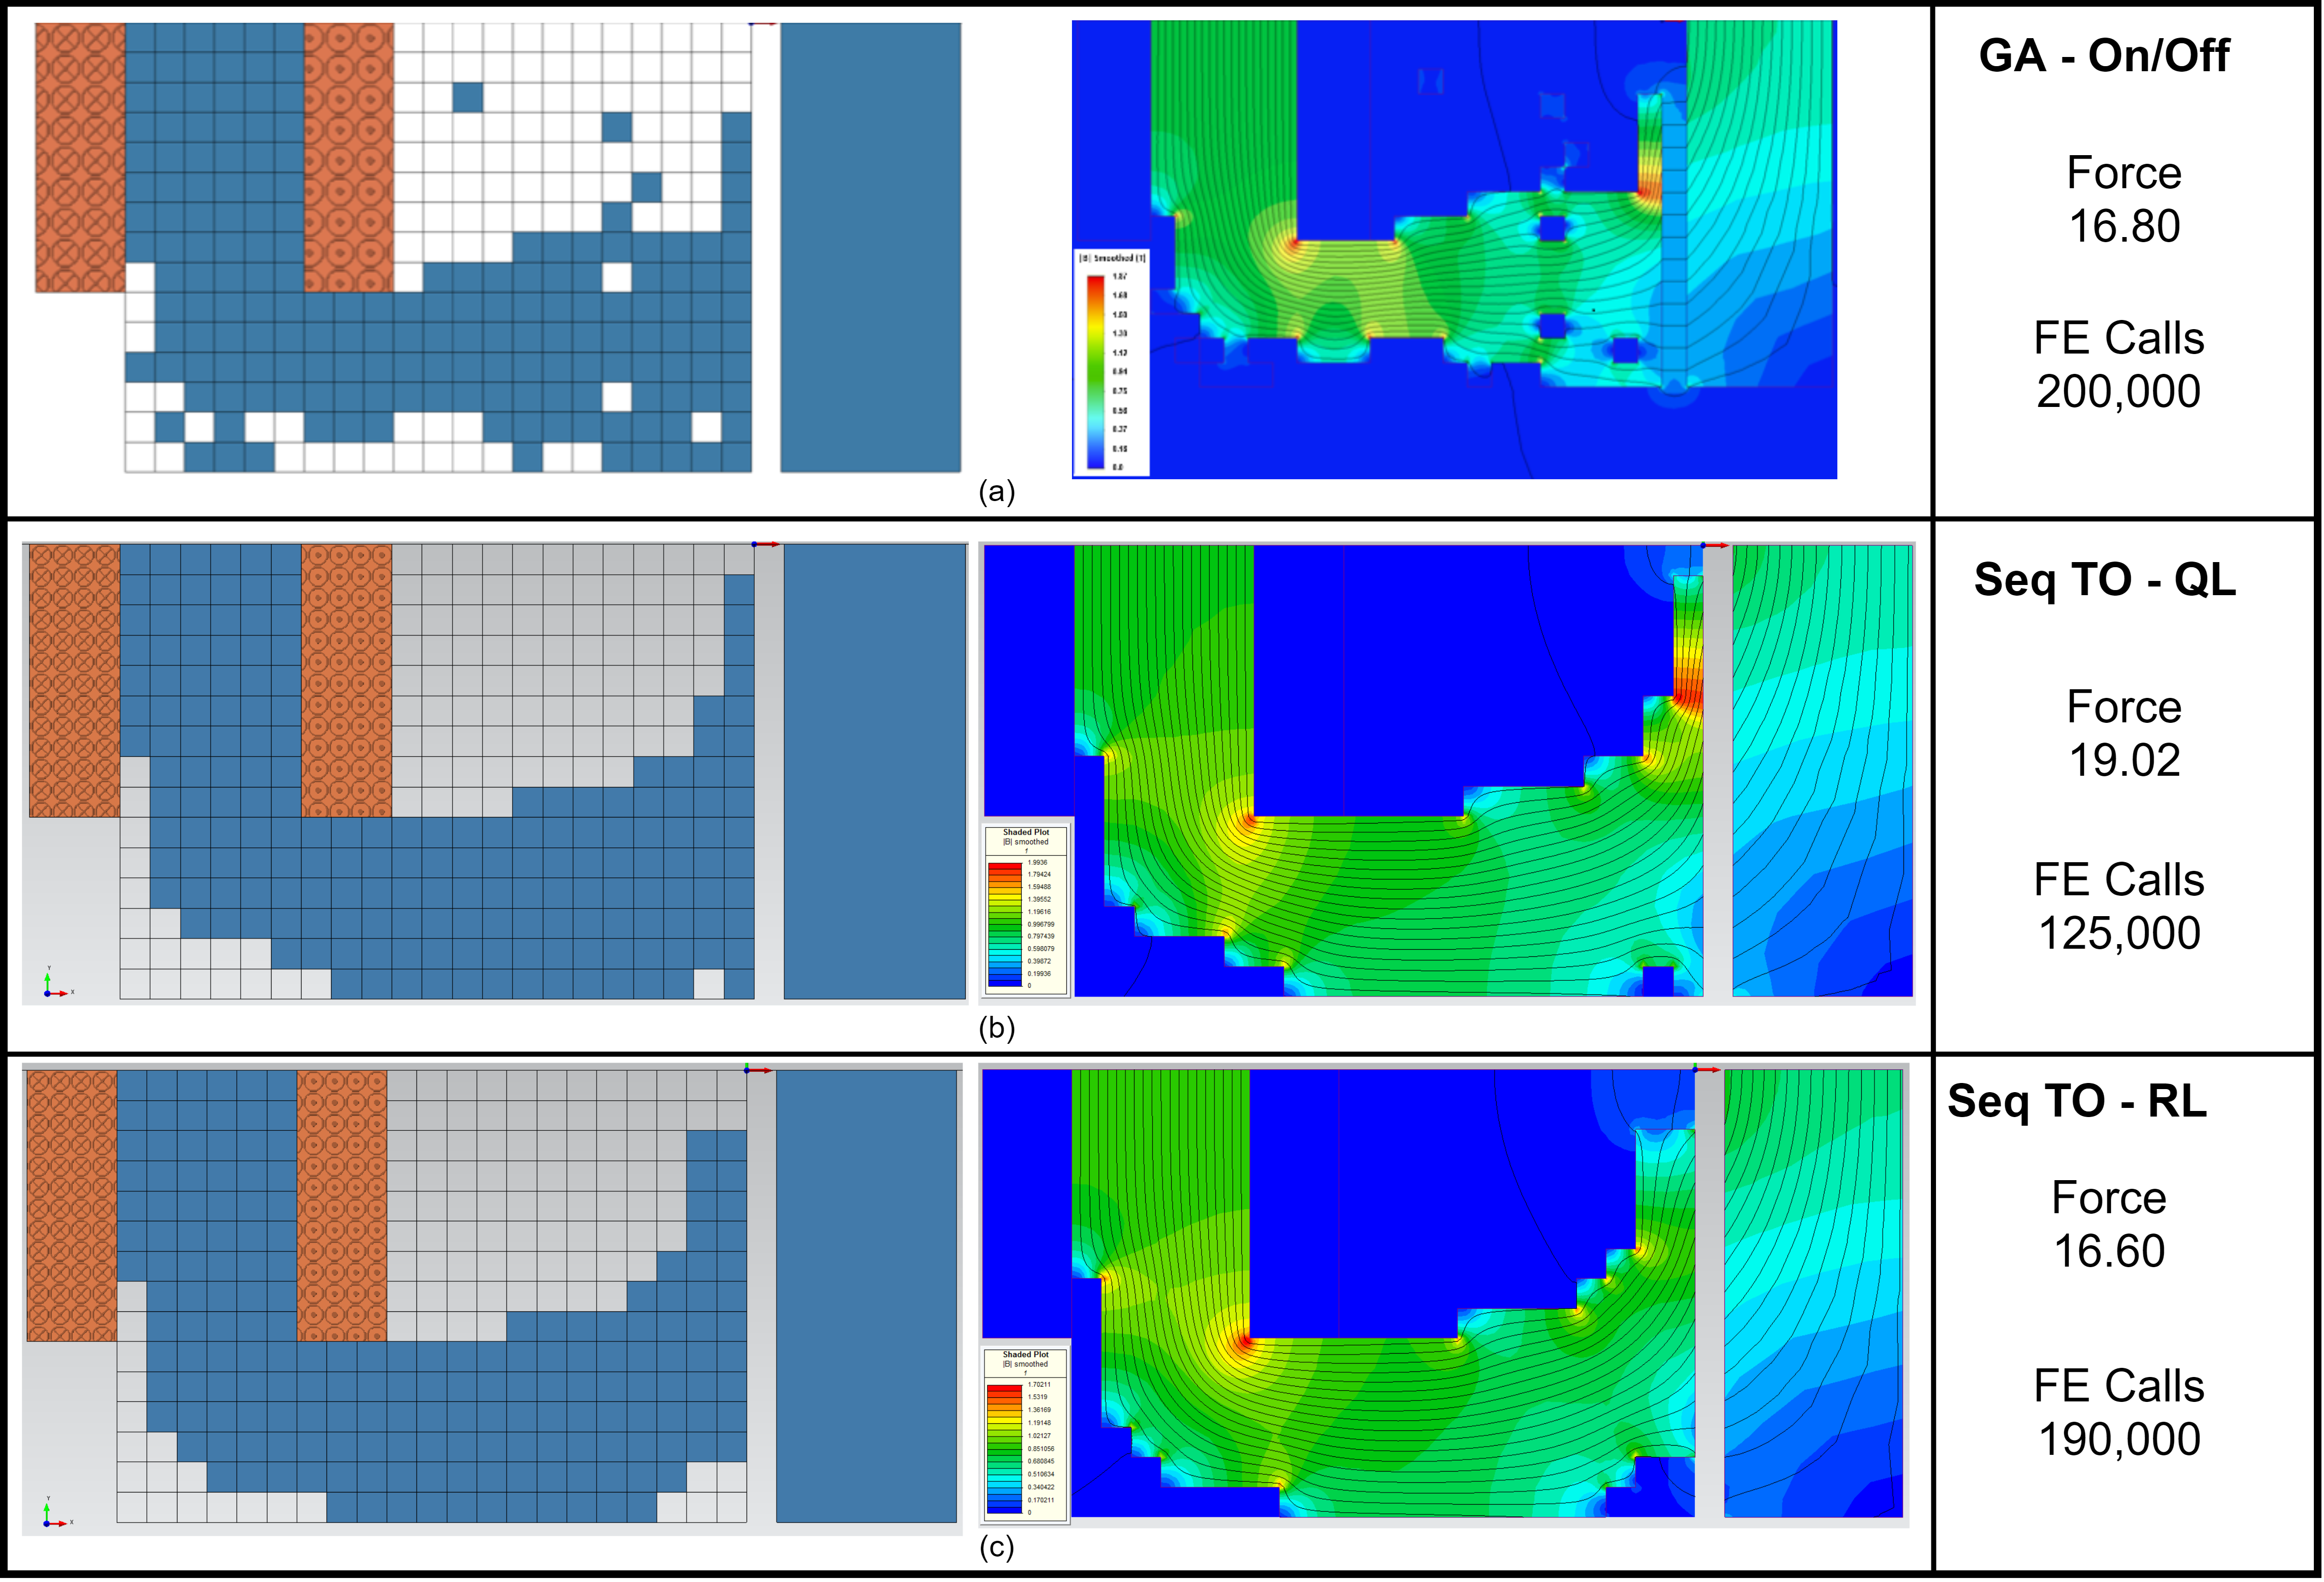
\includegraphics[width=\textwidth]{Figures/Ch_RL/Ccore_0.5A.png}
    \caption{Optimal geometry and B distribution for excitation scenario (1.0 A, 250 Turns) for (a) GA (b) QL based on SeqTO-v1 (c) A2C based on SeqTO-v2.}
    \label{fig:RL_Ccore_0.5A_GeoNB}
\end{figure}

\begin{figure}[h!]
    \centering
    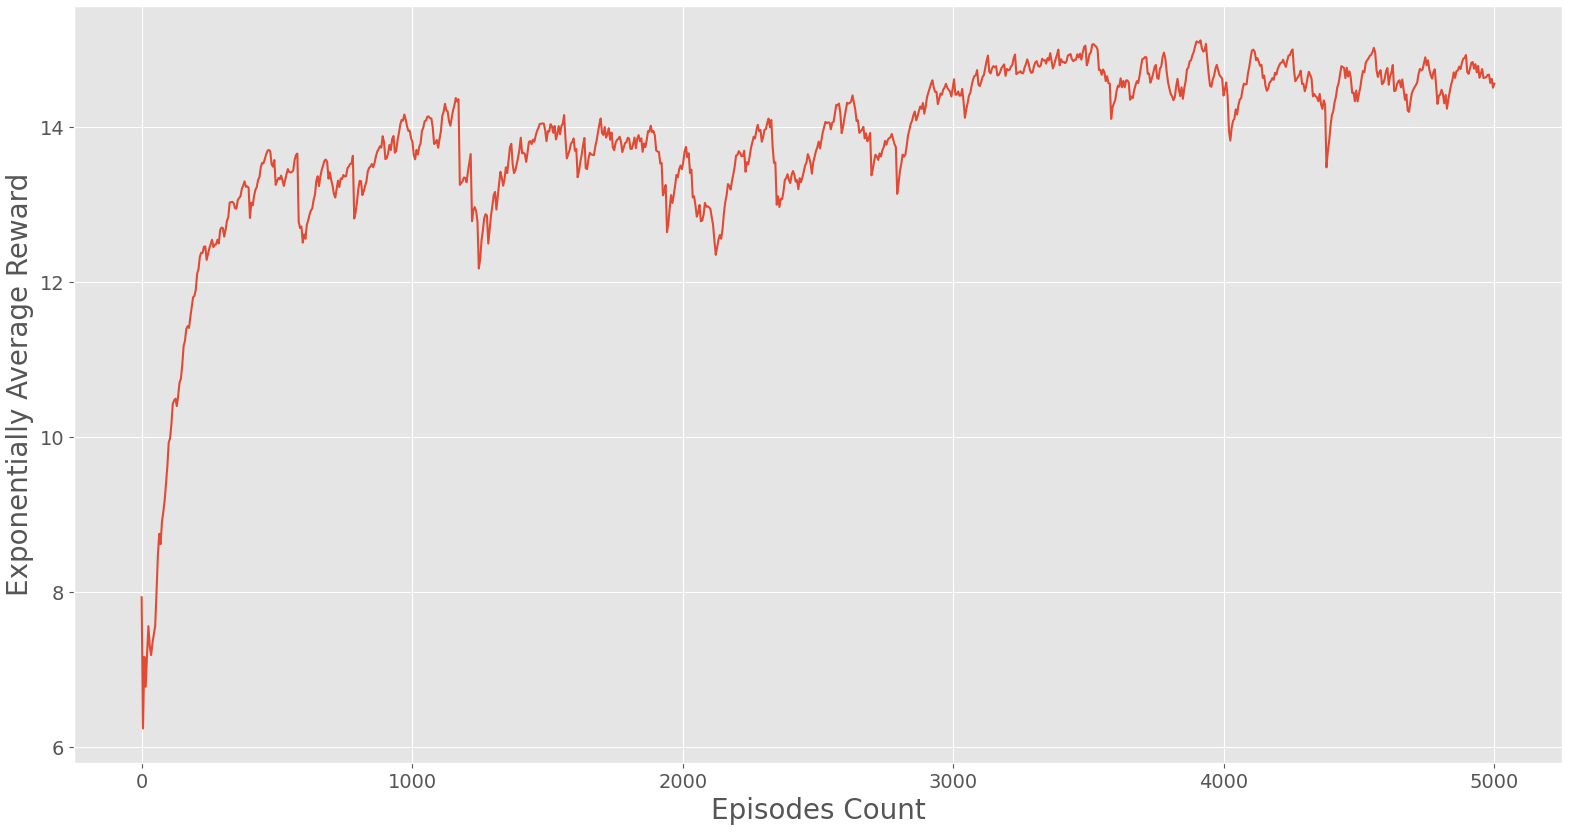
\includegraphics[width=0.85\textwidth]{Figures/Ch_RL/0.5A_A2C.png}
    \caption{Convergence results for 1.0 Amps, 250 Turns}
    \label{fig:RL_convergence_500AT}
\end{figure}

\begin{figure}[h!]
    \centering
    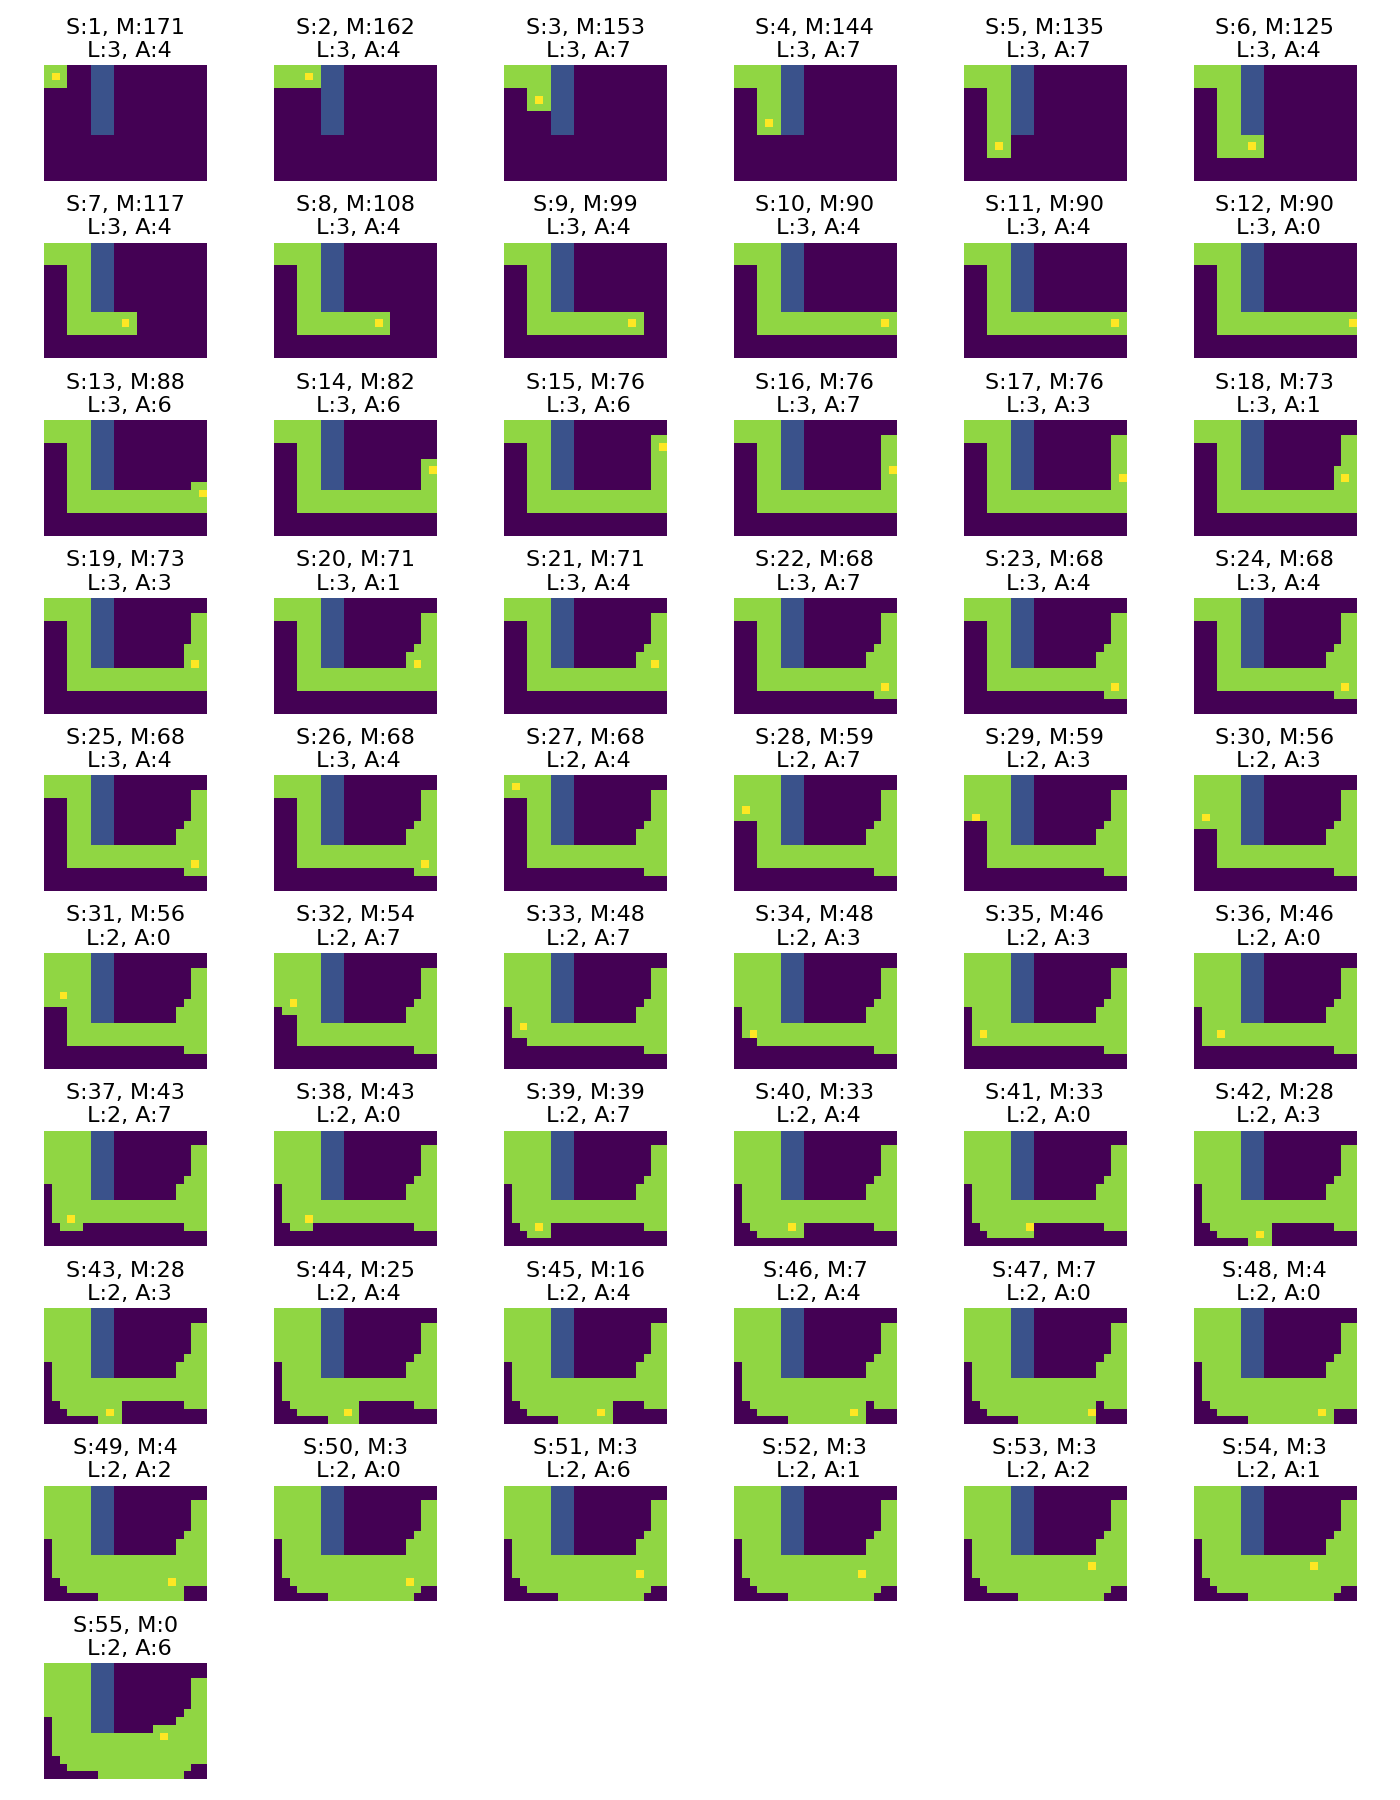
\includegraphics[width=\textwidth]{Figures/Ch_RL/0.50_Count180_NetForce19.02.png}
    \caption{Sequence for optimal geometry for excitation: 1.0 A, 250 Turns. Only the design domain is shown. S: Step No., M: Material left, L: Lives left.}
    \label{fig:RL_Ccore_0.5A_sequence}
\end{figure}

The sequence of actions corresponding to the optimal geometry obtained for this excitation using the A2C agent is shown in Figure \ref{fig:RL_Ccore_0.5A_sequence}. The optimal geometry obtained with a $1\ \times 1$ controller based on QL generates a higher force ($19.02 \hspace{2pt} \hspace{2pt} N$) than the one obtained through an A2C controller ($16.60 \hspace{2pt} \hspace{2pt} N$). As mentioned earlier, the reason can be attributed to the ability of a $1\ \times 1$ controller to place a thin strip of iron close to the air gap, whereas SeqTO-\textit{v2} limits such maneuverability. Since the pointer of the controller cannot move out of the design space, the smallest width of material block is limited to 2 near the boundary of the design space, in the SeqTO-\textit{v2} environment. This can be seen from Step: 12 to 15 in Figure \ref{fig:RL_Ccore_0.5A_sequence}.  

\clearpage
\newpage

\subsubsection{C-core Excitation Scenario 2}
\textit{Coil Current $= 0.75 A$  \& Coil Turns $= 500$}

This scenario is part of the `\textit{test}’ excitation cases i.e., interaction without learning, where the A2C agent did not learn from an environment operating this excitation scenario during the training phase. The GA algorithm and the QL-based agent were directly optimized using the `\textit{test}' case excitation values and results in the optimal design solution. 

Although this `\textit{test}' case was not part of the training for A2C, the agent still managed to obtain a close to optimal ($32.70 \hspace{2pt} N$; $ 6\% $ lower) performance when compared to QL ($34.80 \hspace{2pt} N$) and an improvement over the result obtained using GA (based on On/Off TO) ($32.50 \hspace{2pt} N$). The agent’s performance improves on further tuning of the agent. This re-training is performed as a post-processing step, where the agent is exposed to the excitation scenario (\textit{Coil Current = 0.75 A \& Coil Turns = 500}) and it learns from this experience, i.e., interaction with learning. After this re-training, the agent managed to attain a force magnitude ($34.60 \hspace{2pt} N$) value similar to the QL-based SeqTO-v1 ($1\ \times 1$). Again, the main difference here is the granularity level that can be achieved by the SeqTO-v2 as compared to SeqTO-v1 as the QL managed to achieve the same results with less material and higher effective FE Calls. The optimal results from GA, QL, A2C and A2C(re-train) is shown in Figure \ref{fig:RL_Ccore_0.75A_GeoNB} (a), (b), (c) & (d) respectively, along with their respective magnetic flux density distribution.

\begin{figure}[h!]
    \centering
    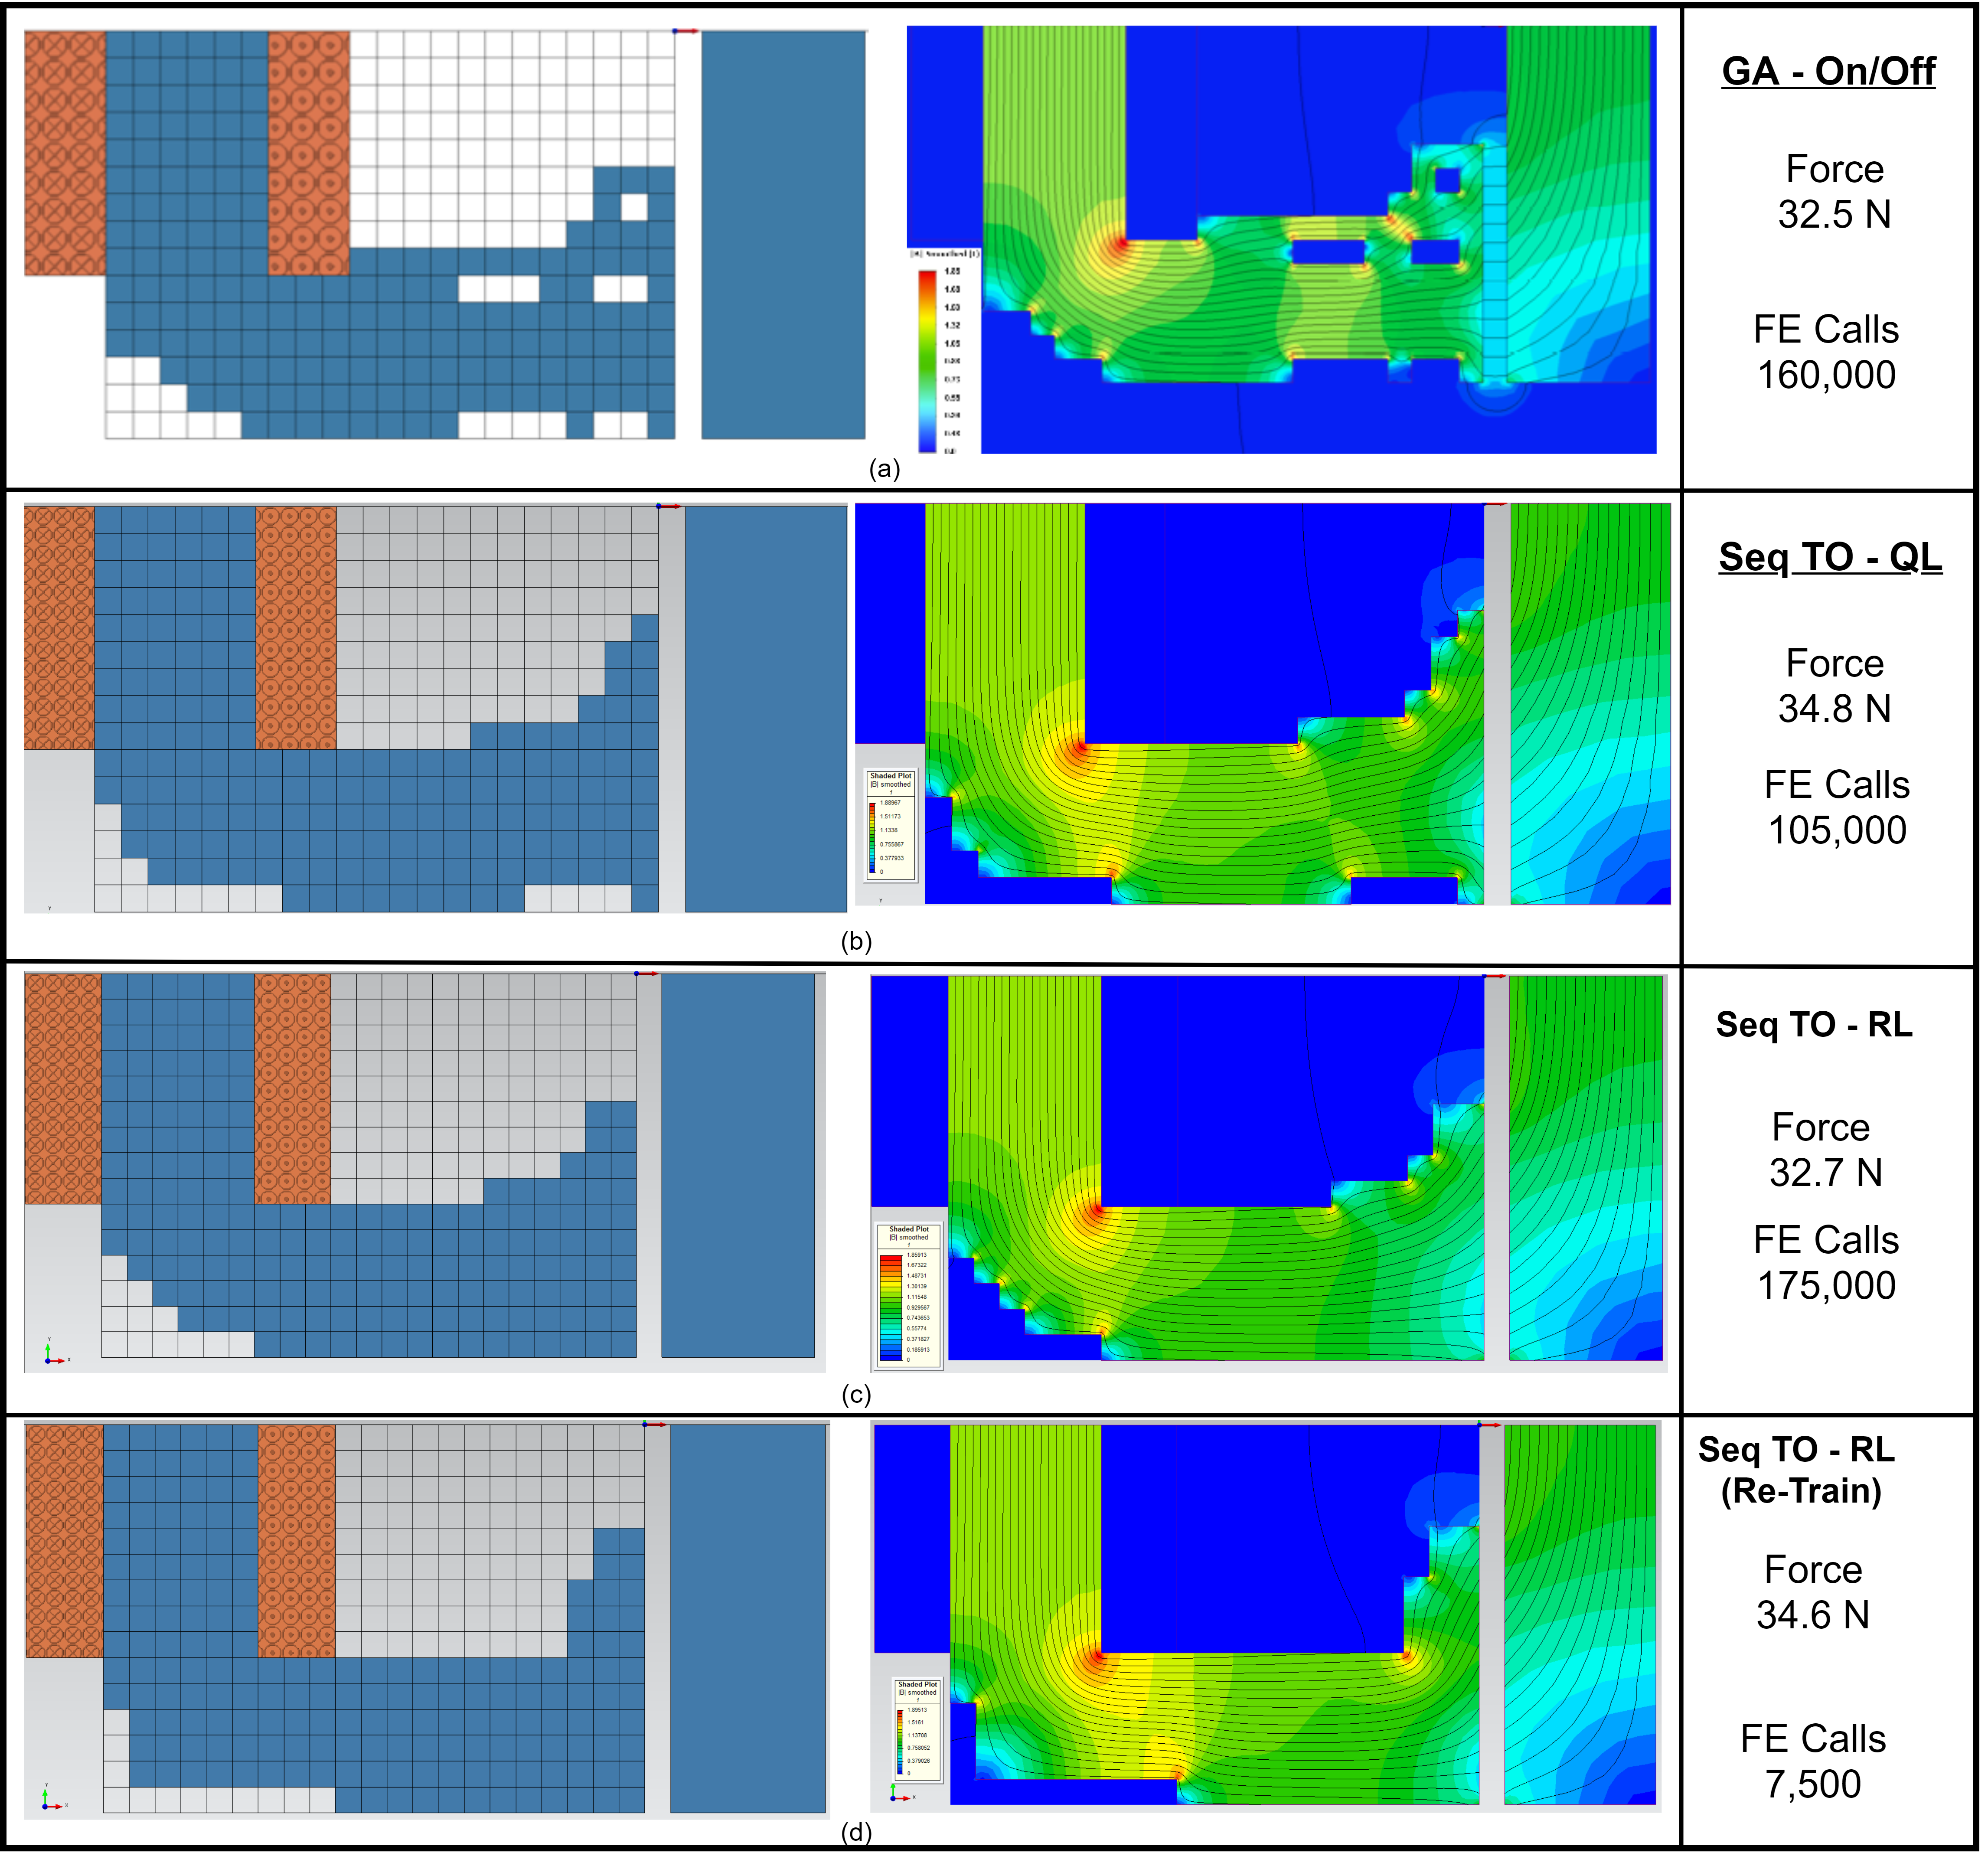
\includegraphics[width=\textwidth]{Figures/Ch_RL/Ccore_0.75A.png}
    \caption{Optimal geometry and B distribution for excitation scenario (0.75 A, 500 Turns) for (a) GA (b) QL based on SeqTO-v1 (c) A2C based on SeqTO-v2 (d) fine-tuned A2C agent.}
    \label{fig:RL_Ccore_0.75A_GeoNB}
\end{figure}

\begin{figure}
    \centering
    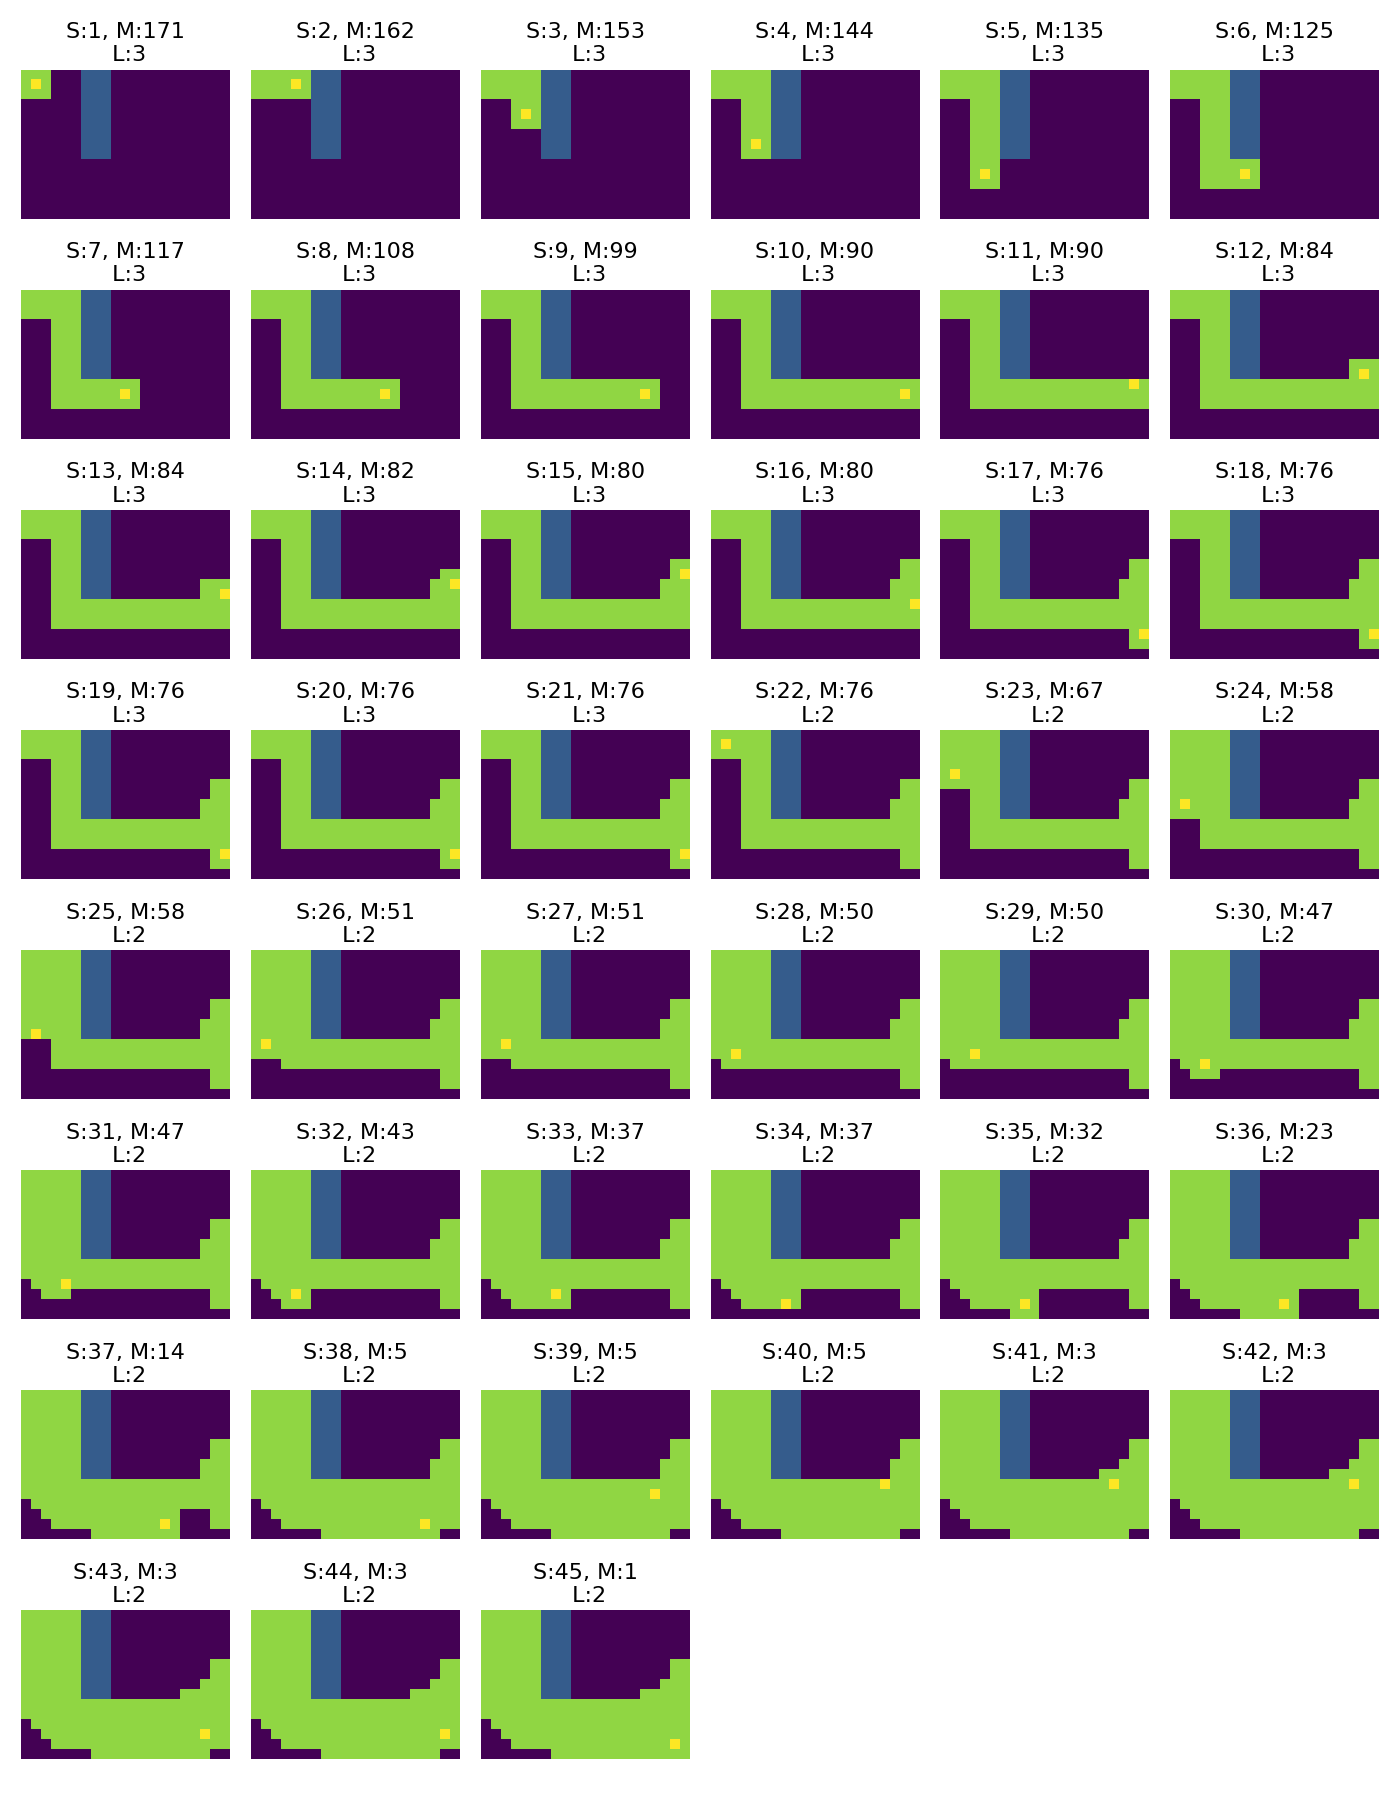
\includegraphics[width=\textwidth]{Figures/Ch_RL/0.75_Count179_NetForce32.7.png}
    \caption{Sequence for optimal geometry for excitation: 0.75 A, 500 Turns. S: Step No., M: Material left, L: Lives left.}
    \label{fig:RL_Ccore_0.75A_sequence}
\end{figure}

The transitional change in the design space due to interaction between the agent and the environment for the excitation scenario (\textit{Coil Current = 0.75 A, Coil Turns = 500}) is shown in Figure \ref{fig:RL_Ccore_0.75A_sequence}. Similar agent behaviour as seen earlier for excitation scenario of \textit{1.0 A, 250 Turns} in Section \ref{section:RL_c_core_excitation_1A_250T}, as can be seen in Figure \ref{fig:RL_Ccore_0.75A_sequence}. The ability to obtain a close to optimal geometry (only $6\%$ lower compared to QL) without ever encountering the excitation condition during the training phase, shows the ability of a function approximator-based A2C agent to generalize to the unseen but relevant input. Further, the number of FEA evaluations needed for re-tuning of the agent for this excitation scenario stands at $7500$. After this re-tuning, the force magnitude obtained from the optimal design reaches $34.60 \hspace{2pt} N$ (comparable to QL with $34.80 \hspace{2pt} N$). This results in significant computational cost reduction as compared to other learning methodologies like QL ($120,000$) and GA ($160,000$) for obtaining similar optimal designs, without a compromise on the performance.
An observation that highlights the capability of the agent's maneuverability can be seen in Figure \ref{fig:RL_Ccore_0.75A_sequence} (step: 13), where the agent uses the boundary of the design domain to place 2 elements and follows up with 4 elements each in the next couple of steps (step: 14 -15). This is possible as the pointer of the controller stays inside the design domain but part of the $3\ \times 3$ block gets trimmed out as it falls out of the design space. The agent uses this capability to save some material. Later in the episode, it wastes four steps (Step: 23 to 26) trying to move out of the design domain and loses a life (L: $3\ \rightarrow 2$). This places the controller back at the origin and now the agent adds magnetic material where the design is severely affected by magnetic saturation. The agent learns to exploit the MDP dynamics where it receives a penalty for moving out of the domain, but the trade-off is being able to move back to the origin and deal with the saturation in the region of material placed near the coil.

\clearpage
\newpage

\begin{figure}[h!]
    \centering
    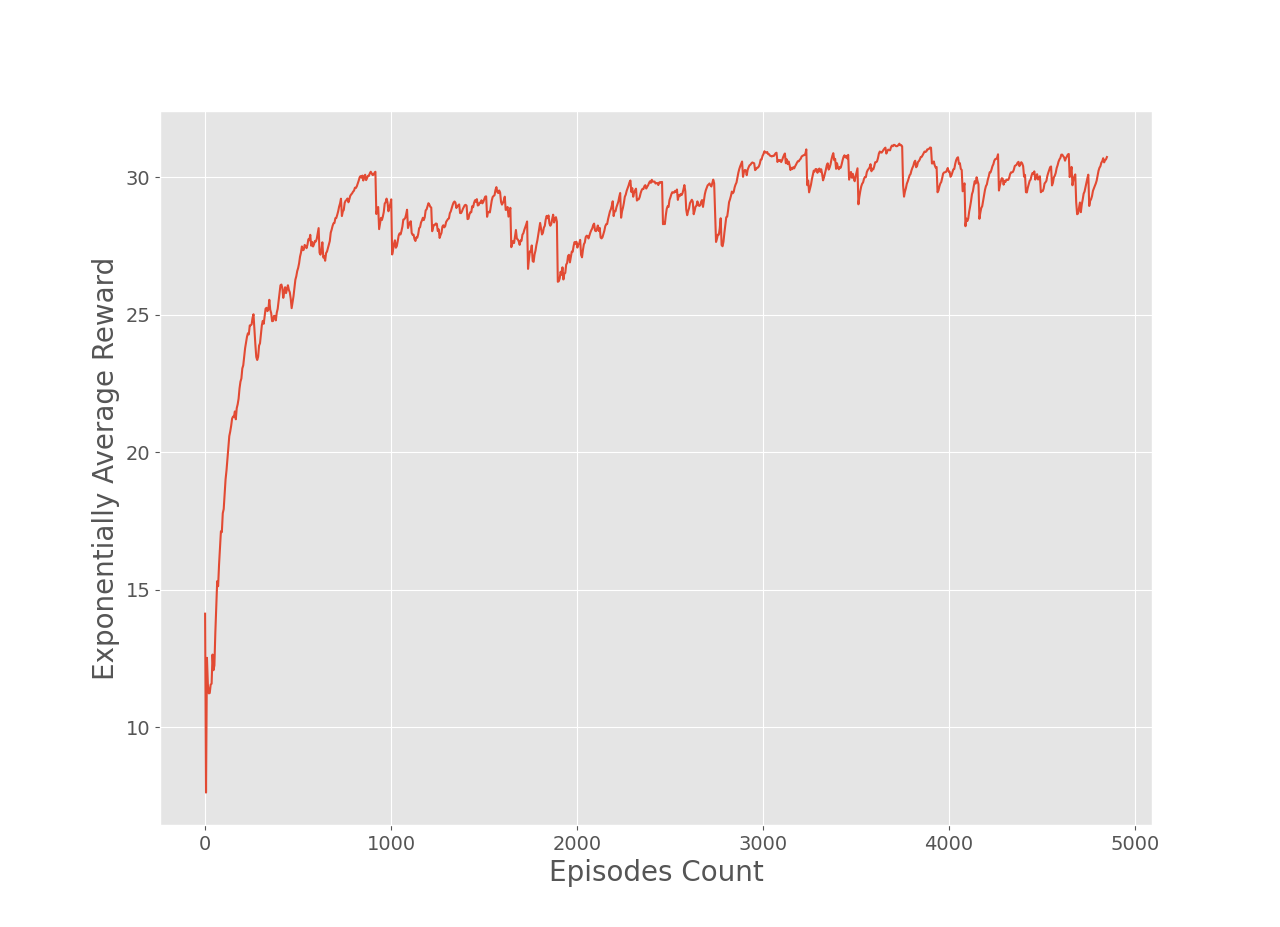
\includegraphics[width=0.75\textwidth]{Figures/Ch_RL/0.75A_RL.png}
    \caption{Convergence results for 0.75 Amps, 500 Turns.}
    \label{fig:RL_convergence_75Amps}
\end{figure}

\subsubsection{C-core Excitation Scenario 3}
Coil Current $= 1.5 $A \\Coil Turns $= 500$ 

For \textit{Coil current $= 1.5$ A \& Coil  Turns $= 500$}, it is observed that all the three algorithms ended up with the core design that resembles the conventional C-core design geometry. Significantly, for cases with an excitation of \textit{500 Amp-Turns} and beyond, the effect of saturation is dominant, and based on the information present in the flux distribution and the excitation level, the agent can form a policy to tackle the phenomenon of material non-linearity.

\begin{figure}[h!]
    \centering
    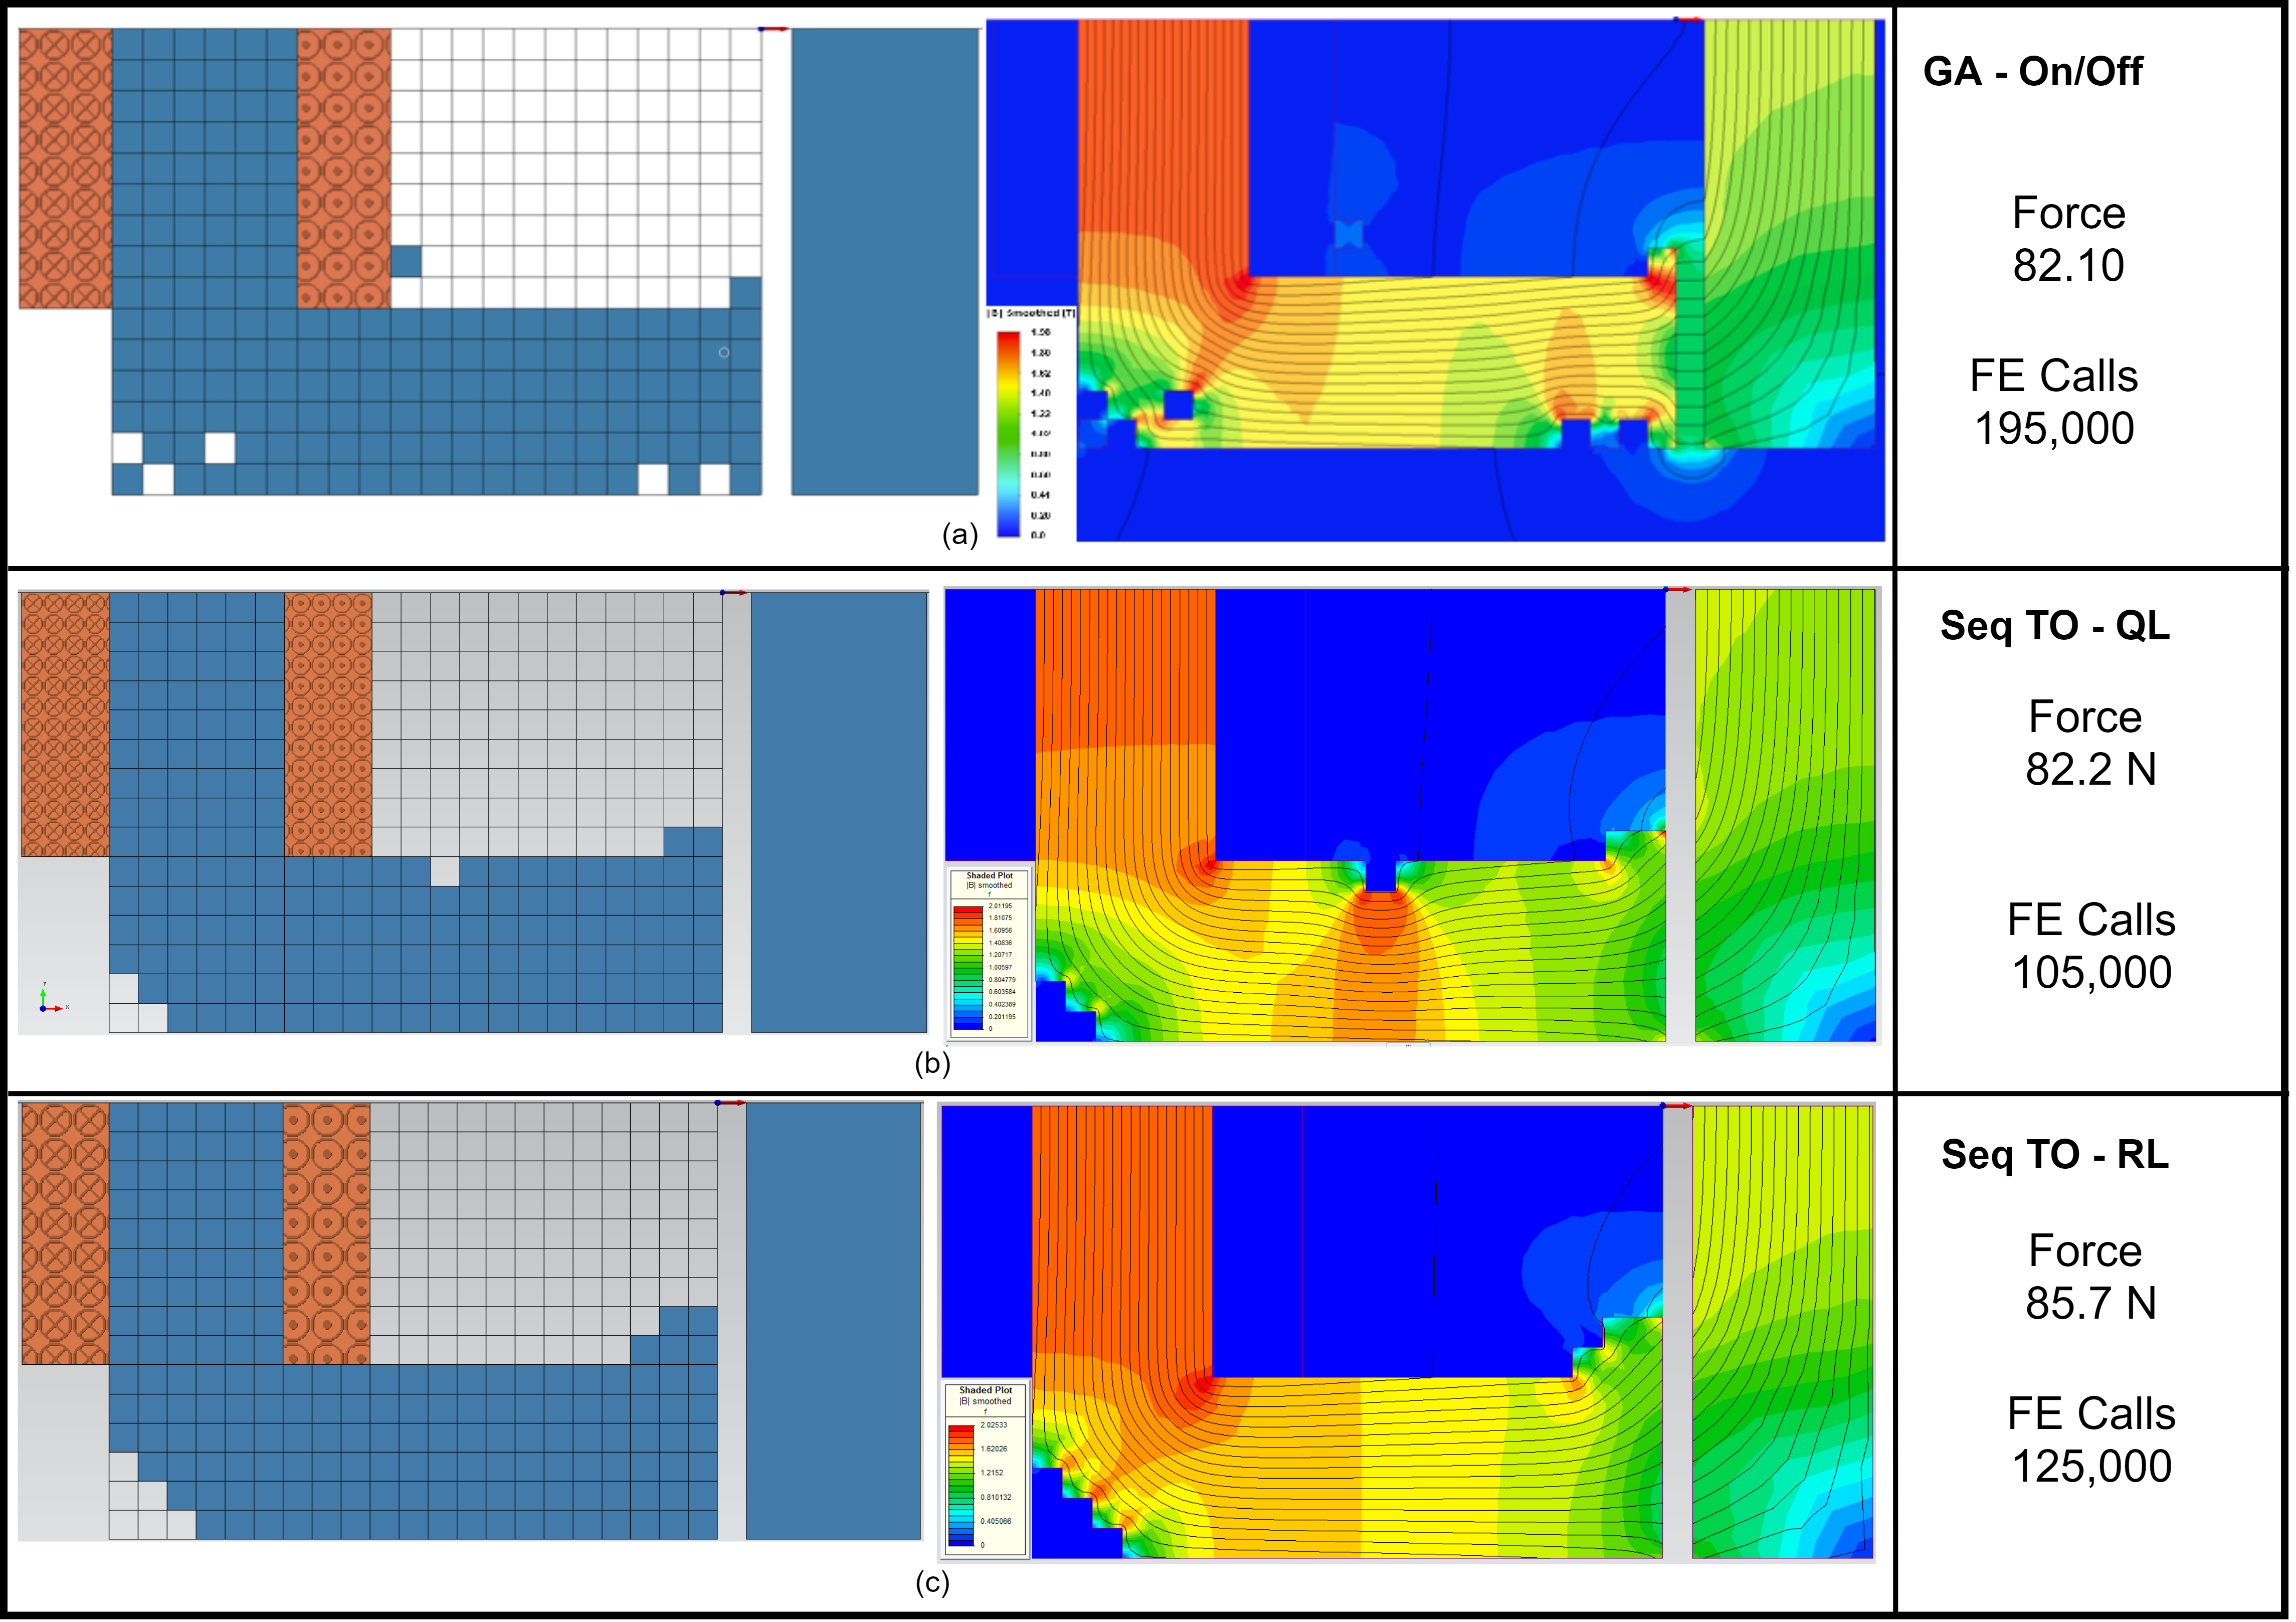
\includegraphics[width=\textwidth]{Figures/Ch_RL/Ccore_1.5A.png}
    \caption{Optimal geometry and B distribution for excitation scenario (1.5 A, 500 Turns) for (a) GA (b) QL based on SeqTO-v1 (c) A2C based on SeqTO-v2.}
    \label{fig:RL_Ccore_1.5A_GeoNB}
\end{figure}

\begin{figure}[h!]
    \centering
    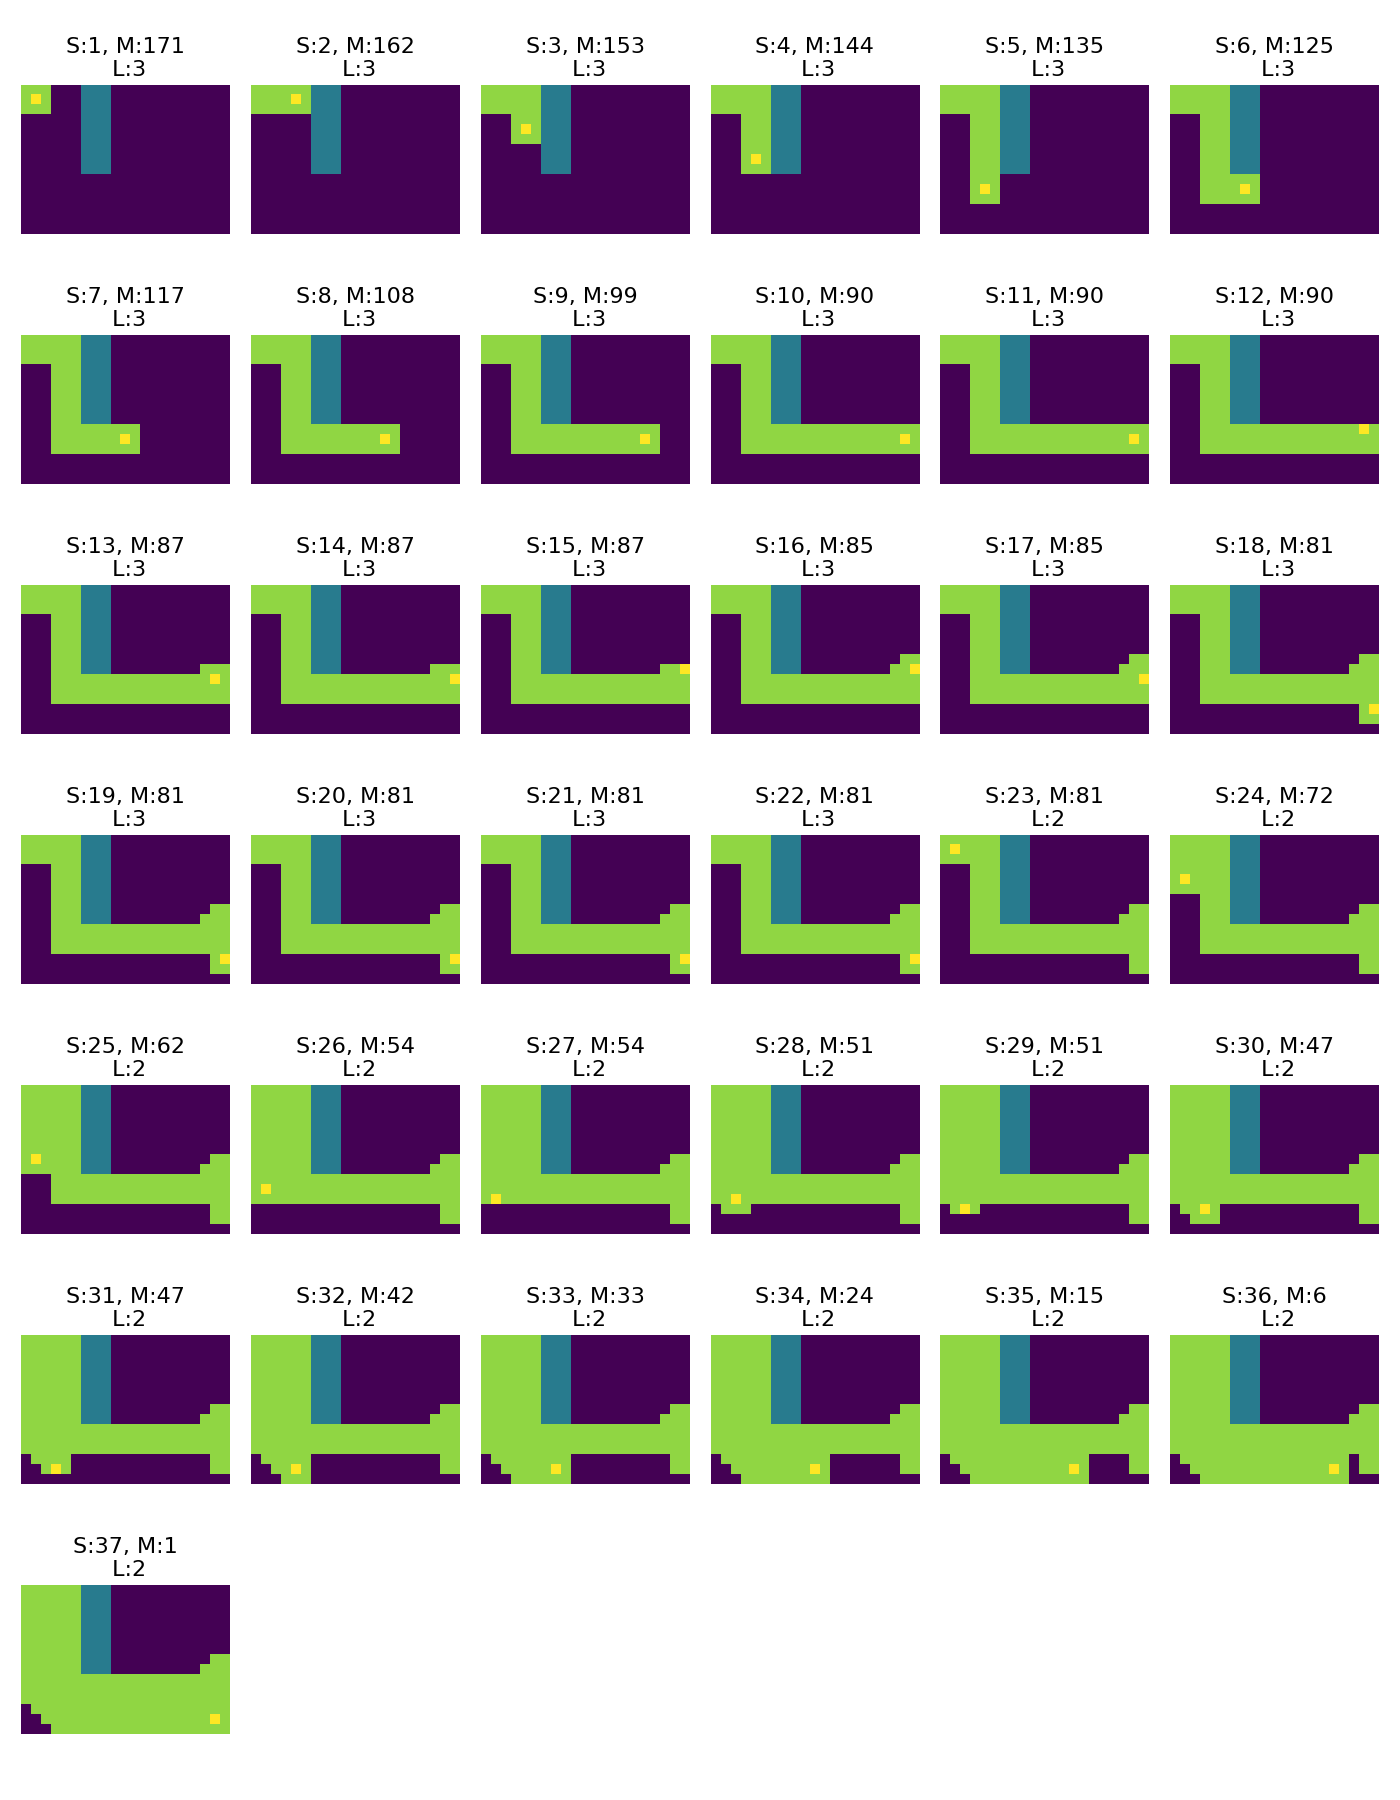
\includegraphics[width=0.95\textwidth]{Figures/Ch_RL/1.50_Count179_NetForce88.02.png}
    \caption{Sequence for optimal geometry for excitation: 1.5 A, 500 Turns. S: Step No., M: Material left, L: Lives left.}
    \label{fig:RL_Ccore_1.5A_sequence}
\end{figure}

\clearpage
\newpage

\begin{figure}[h!]
    \centering
    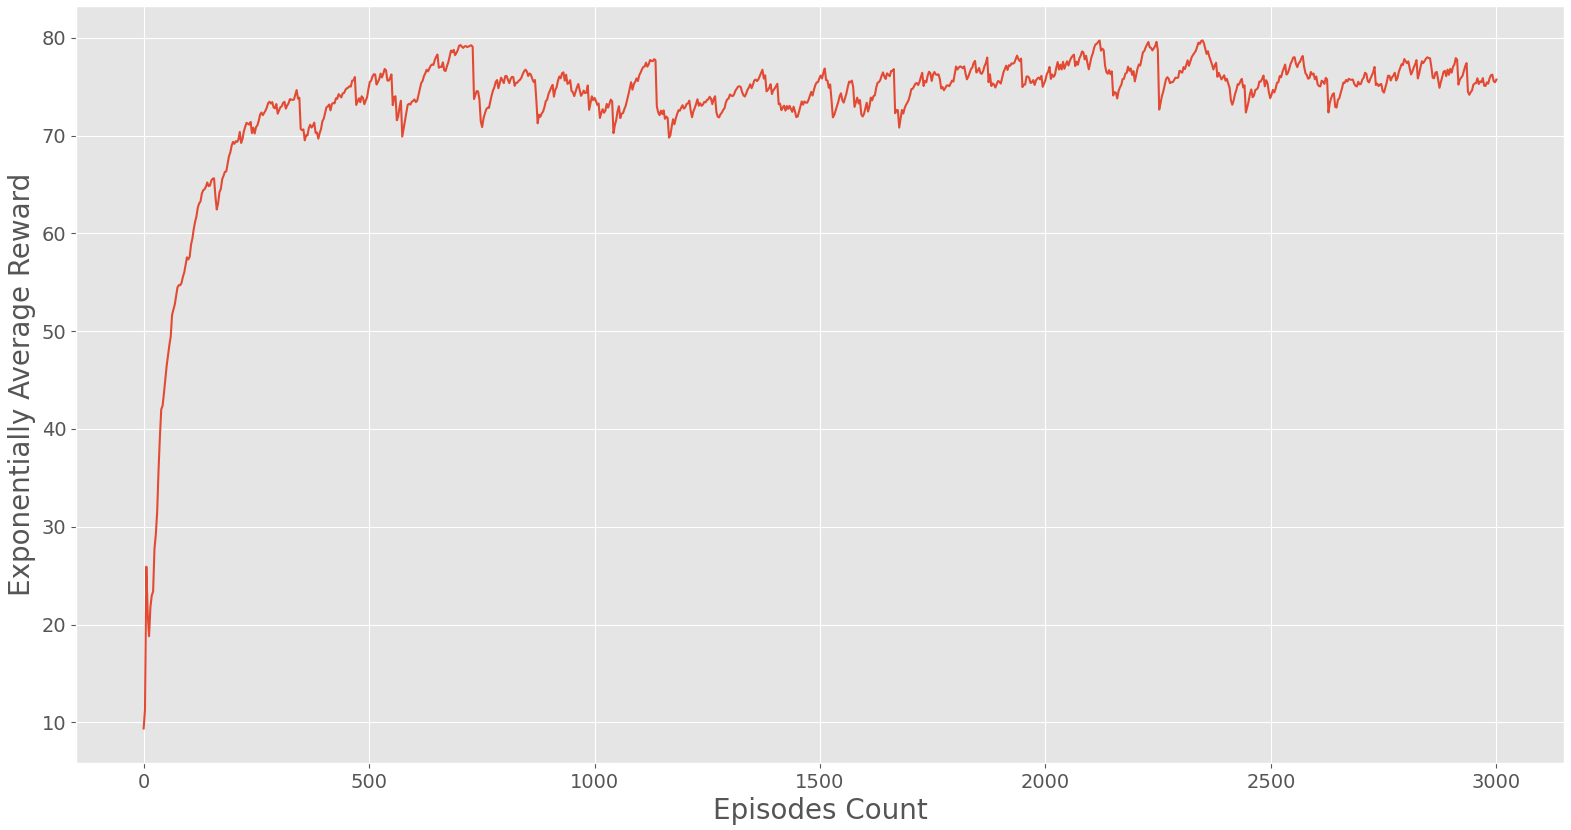
\includegraphics[width=0.75\textwidth]{Figures/Ch_RL/1.5A_A2C.png}
    \caption{Convergence results for 1.5 Amps, 500 Turns.}
    \label{fig:RL_convergence_750AT}
\end{figure}

\subsubsection{Other C-core excitation scenarios}

The analysis of other scenarios is similar to the three scenarios discussed earlier in this section. For excitation scenarios of (\textit{1.75 A \& 500 Turns}) and (\textit{2.0 A \& 500 Turns}), there is not much margin for topological change as compared to the conventional geometry of the C-core (shown in Figure \ref{fig:RL_c_core_conventional_latex}). For both these scenarios, the conventional geometry is one of the solutions provided by the A2C algorithm, as can be seen in Figure \ref{fig:RL_Ccore_1.75A} (b) and \ref{fig:RL_Ccore_2.0A} (b) for 1.75 A and 2.0 A respectively. Based on the agent’s action, it can be concluded that the optimal design does not deviate much from the conventional geometry for higher values of excitation (750 Amp-Turns onwards). This is in agreement with the optimal solutions obtained using other optimization algorithms (GA and QL). 

\begin{figure}[h!]
    \centering
    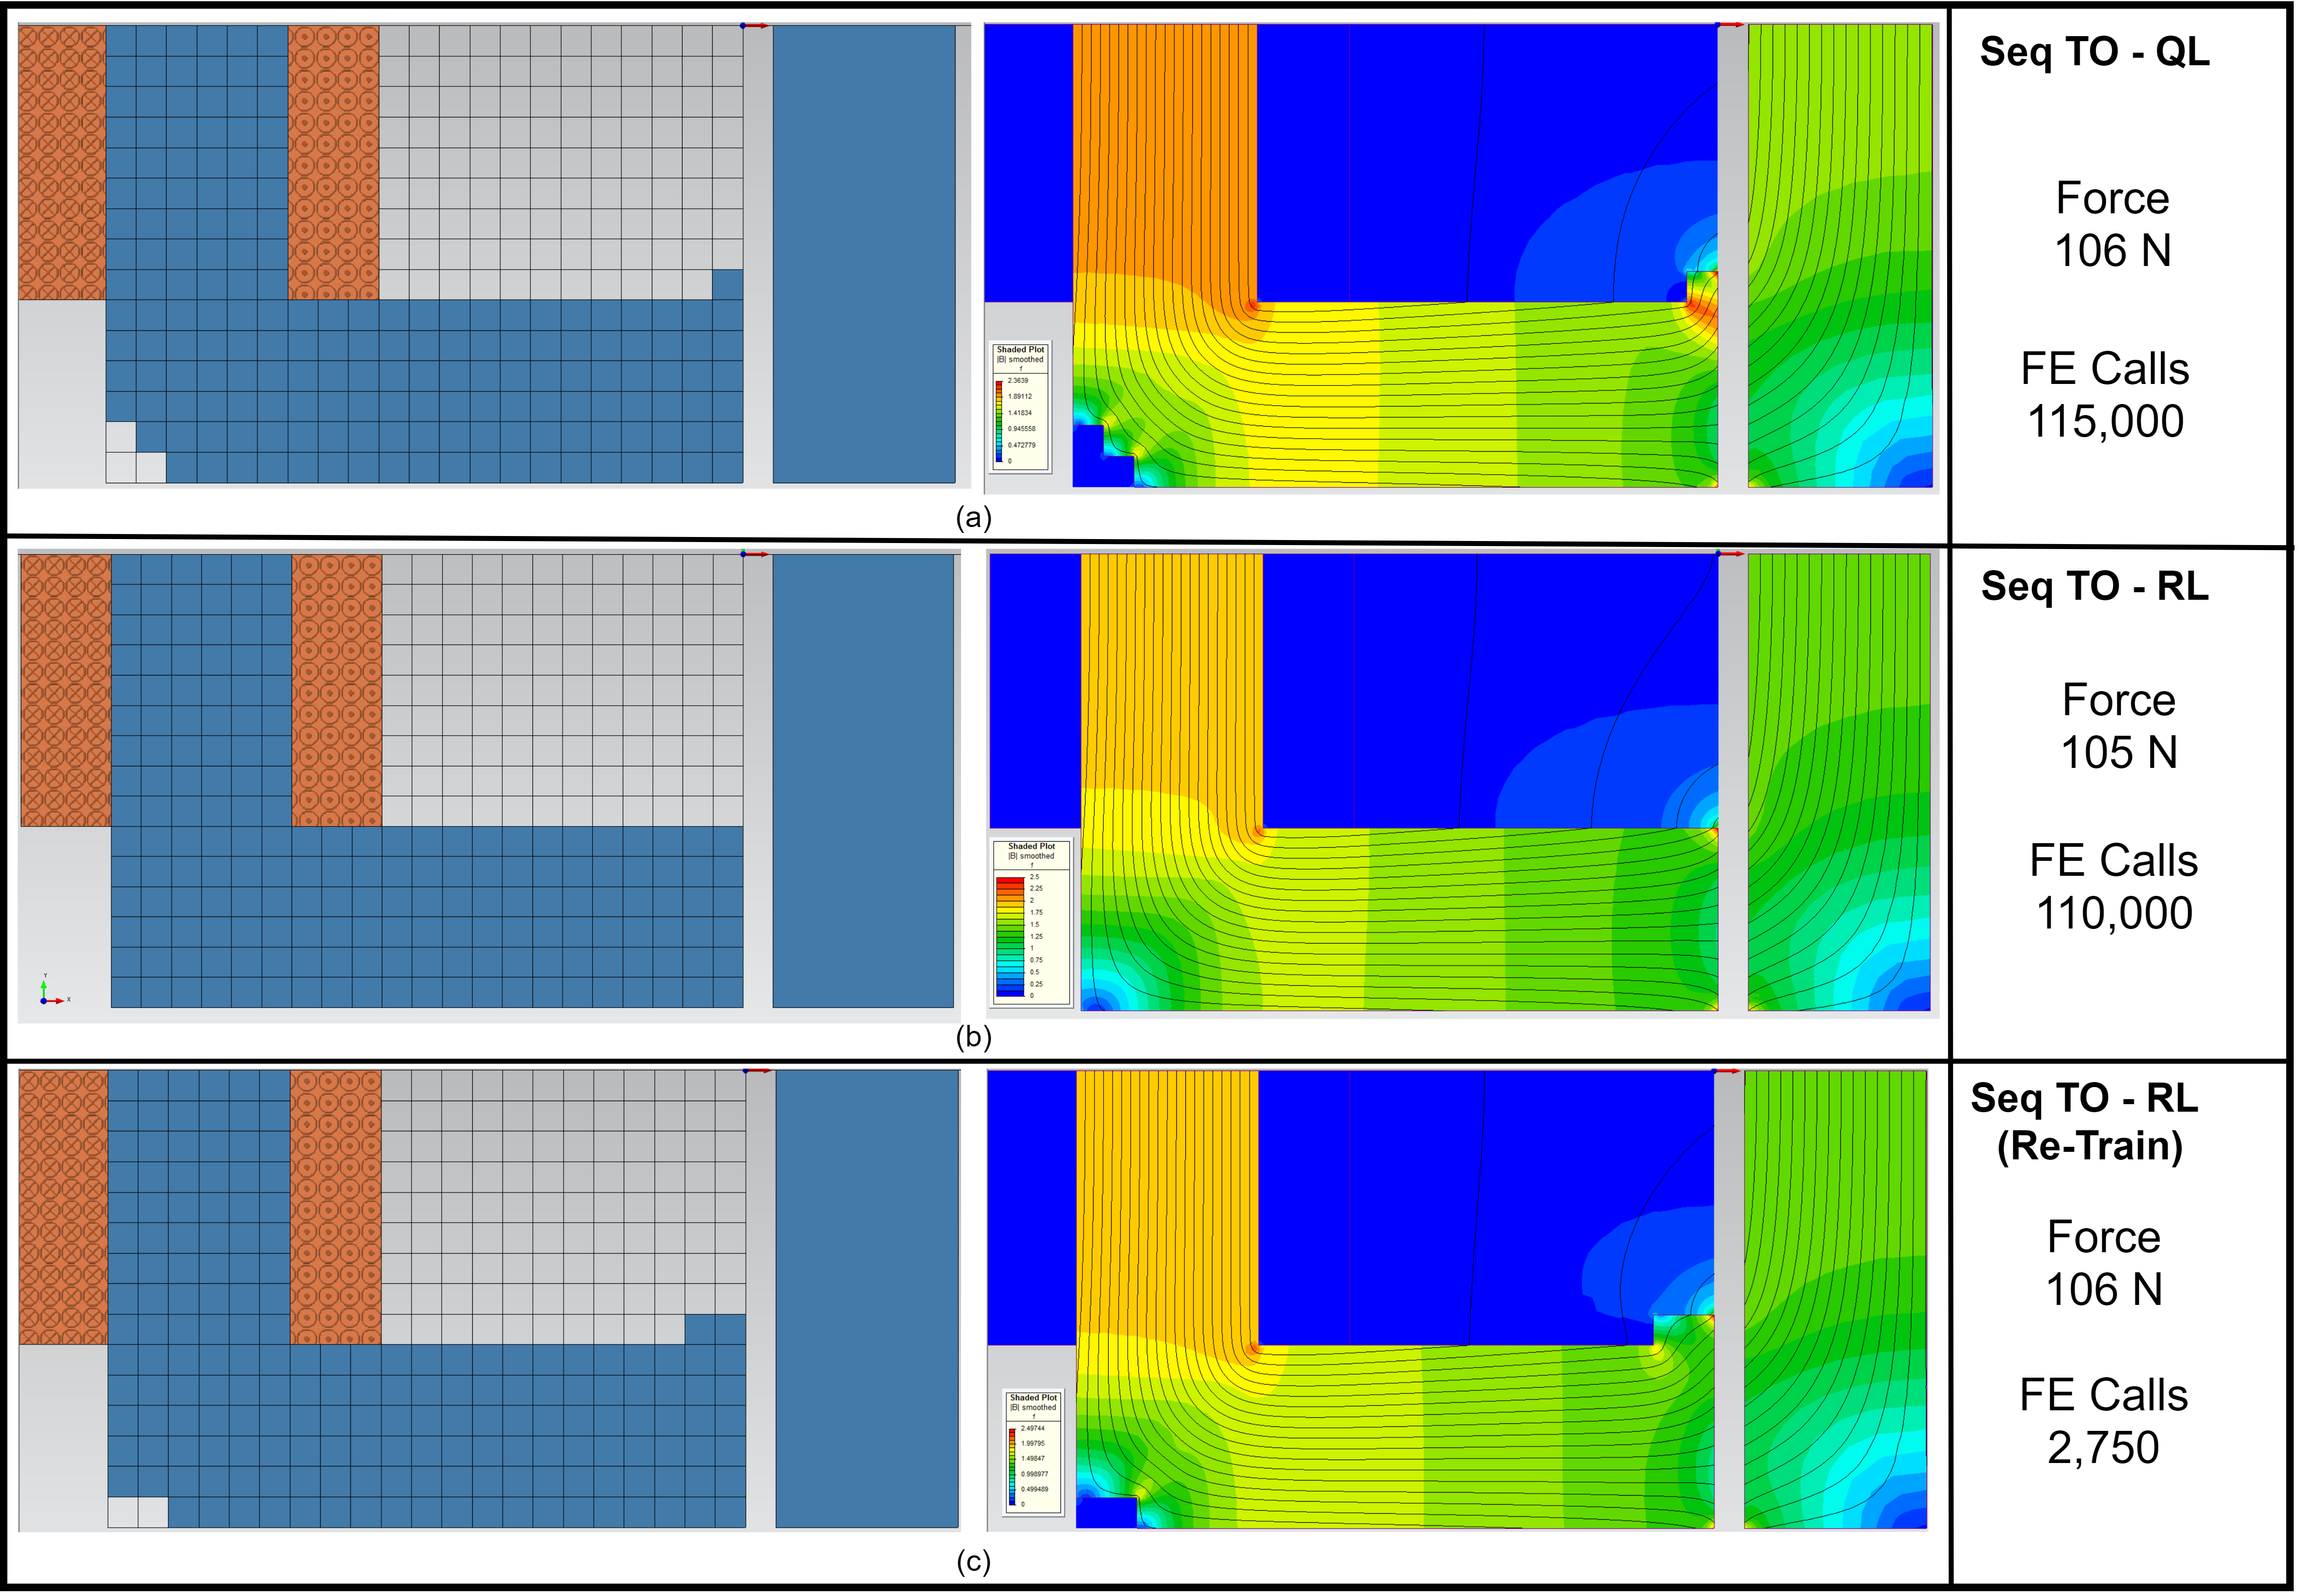
\includegraphics[width=\textwidth]{Figures/Ch_RL/Ccore_2.0A.png}
    \caption{Optimal geometry and B distribution for excitation scenario (2.0 A, 500 Turns) for (a) GA (b) QL based on SeqTO-v1 (c) A2C based on SeqTO-v2.}
    \label{fig:RL_Ccore_2.0A}
\end{figure}

\begin{figure}[h!]
    \centering
    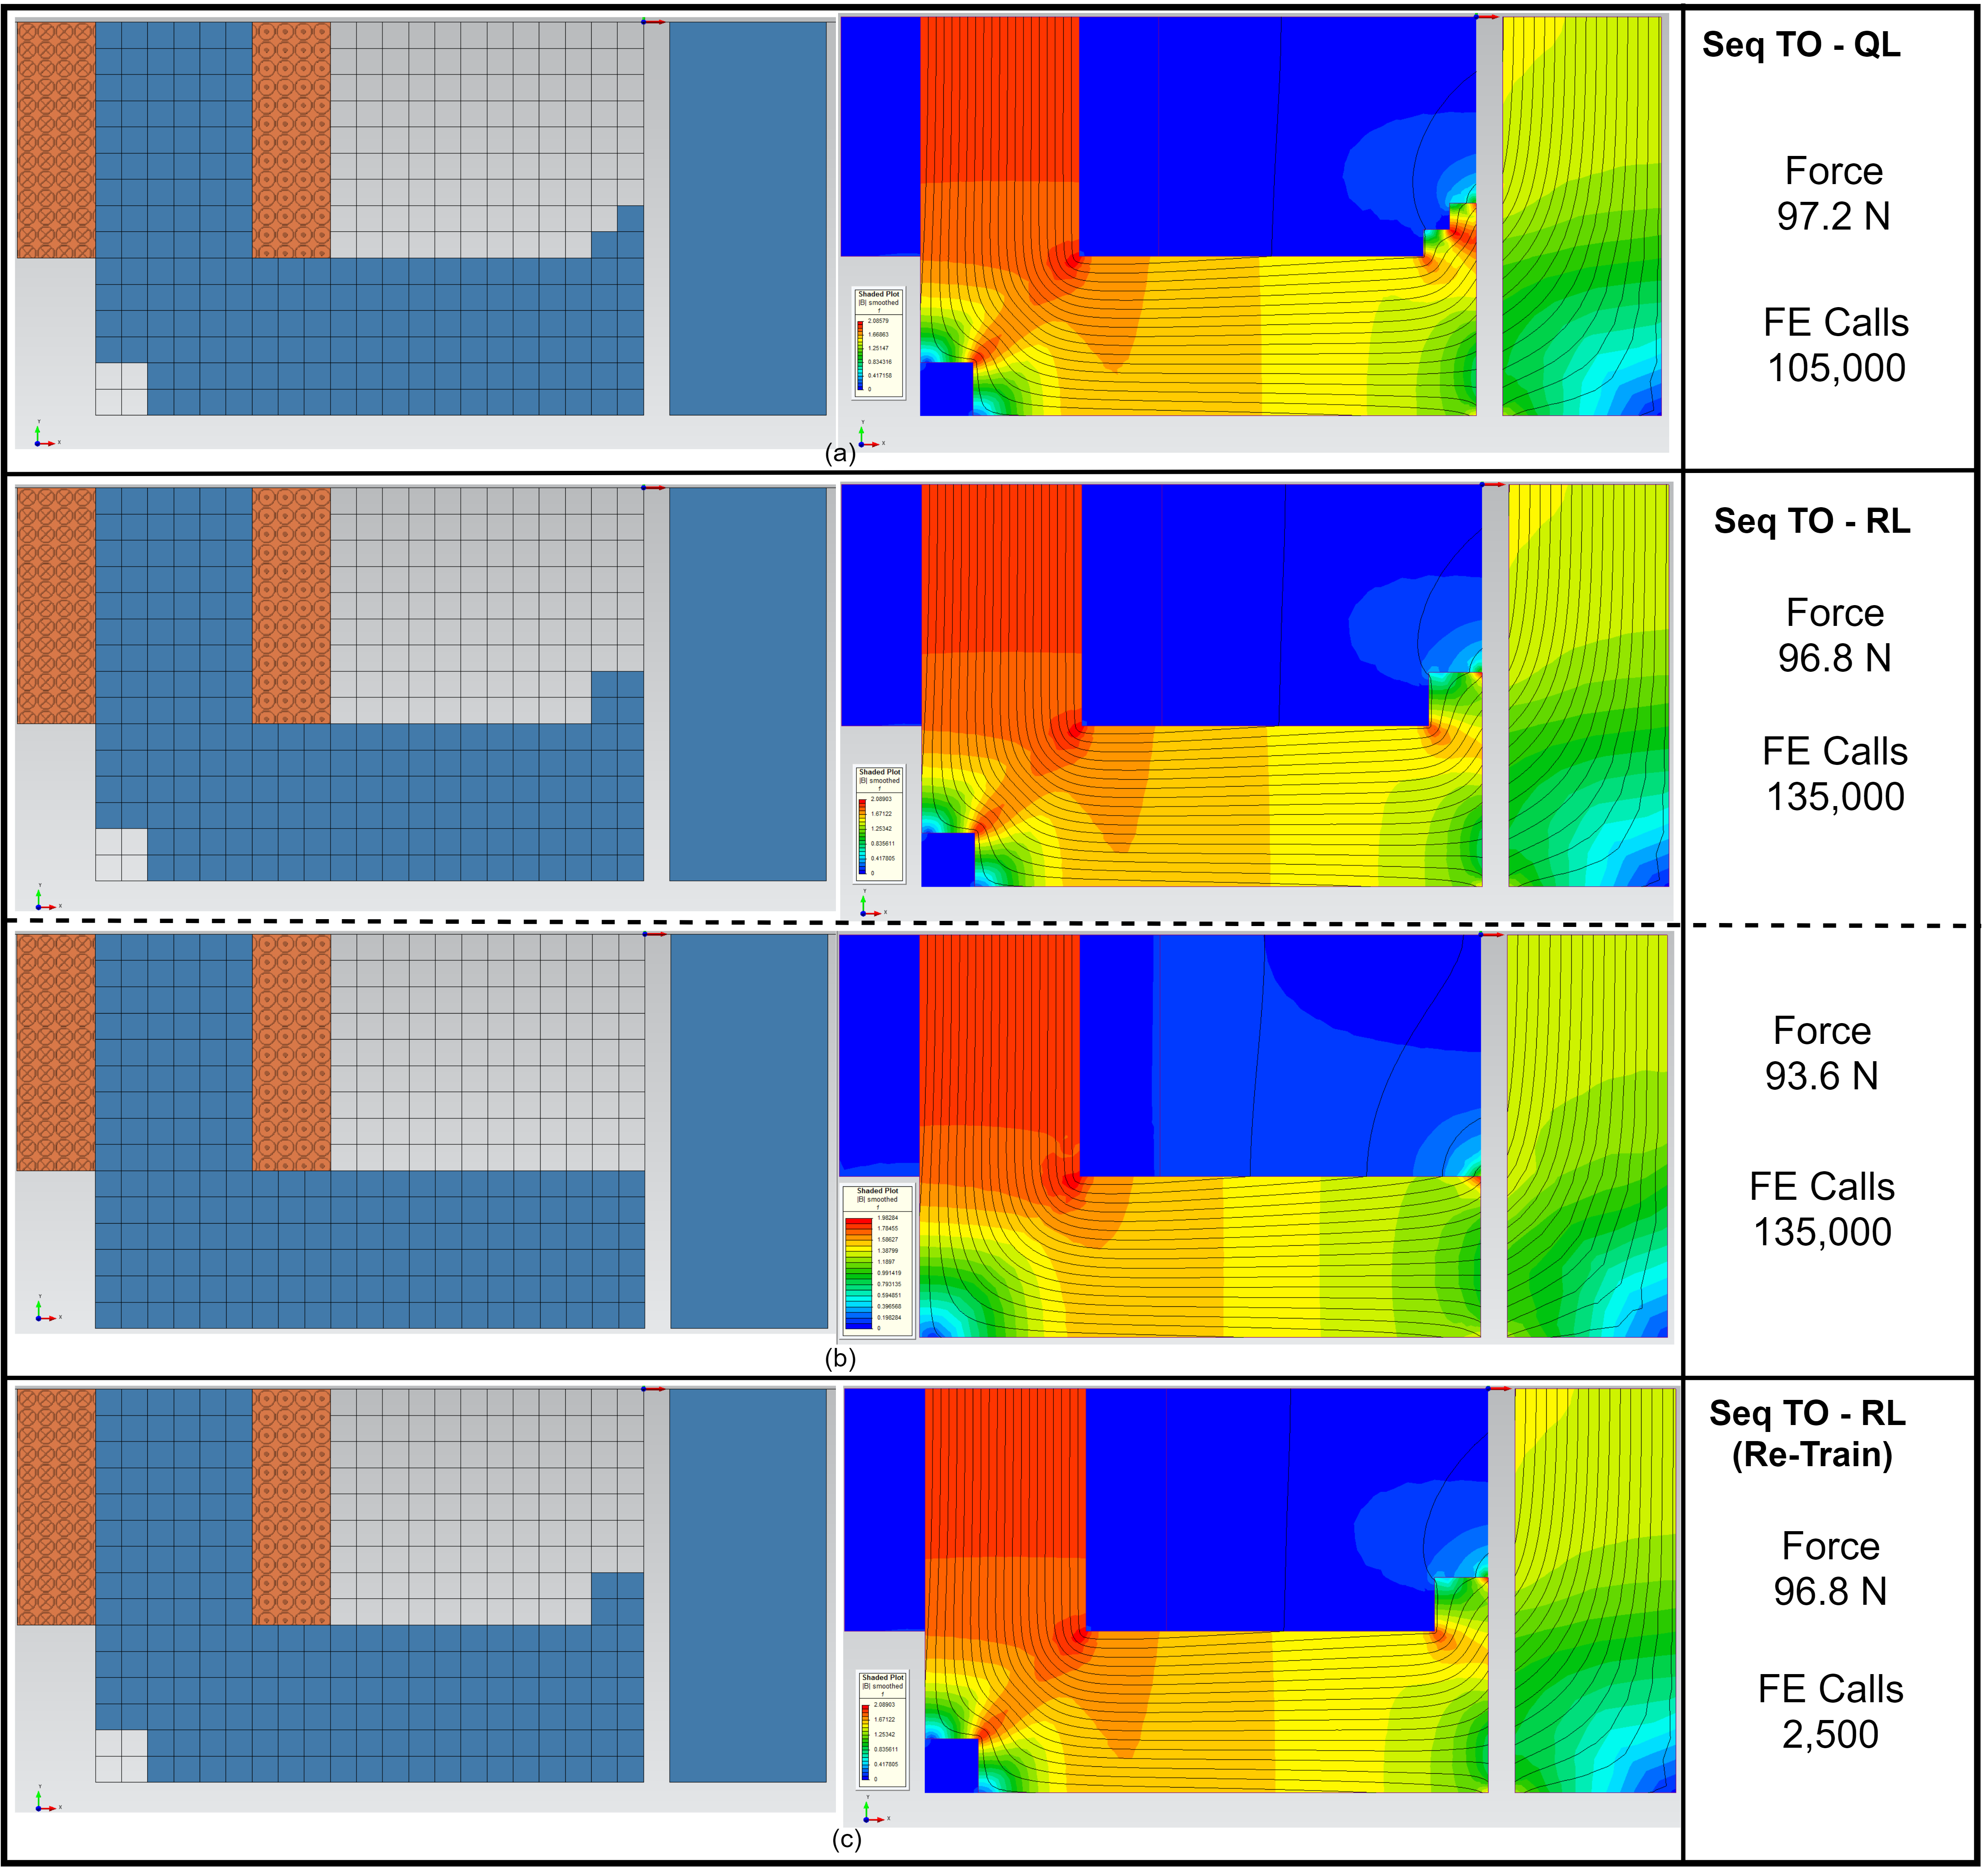
\includegraphics[width=\textwidth]{Figures/Ch_RL/Ccore_1.75A.png}
    \caption{Optimal geometry and B distribution for excitation scenario (1.75 A, 500 Turns) for (a) GA (b) QL based on SeqTO-v1 (c) A2C based on SeqTO-v2.}
    \label{fig:RL_Ccore_1.75A}
\end{figure}

The excitation scenario: \textit{1.25 A \& 500 Turns} shows resemblance to \textit{1.5 A \& 500 Turns}.  A comparison of optimal geometries from GA (On/Off), Tabular QL (SeqTO-\textit{v1}) and A2C (SeqTO-\textit{v2}), is shown in Figure \ref{fig:RL_Ccore_1.25A}. In contrast, the agent shows a significant change in topology for lower values of excitation as can be seen for the scenario: \textit{0.25A \& 500 Turns} in Figure \ref{fig:RL_Ccore_0.25A}. The reason being that the magnetic material placed near the coils is no longer easily saturated and the agent can aggressively place more material near the airgap facing the armature, forcing more flux out laterally.

\begin{figure}[h!]
    \centering
    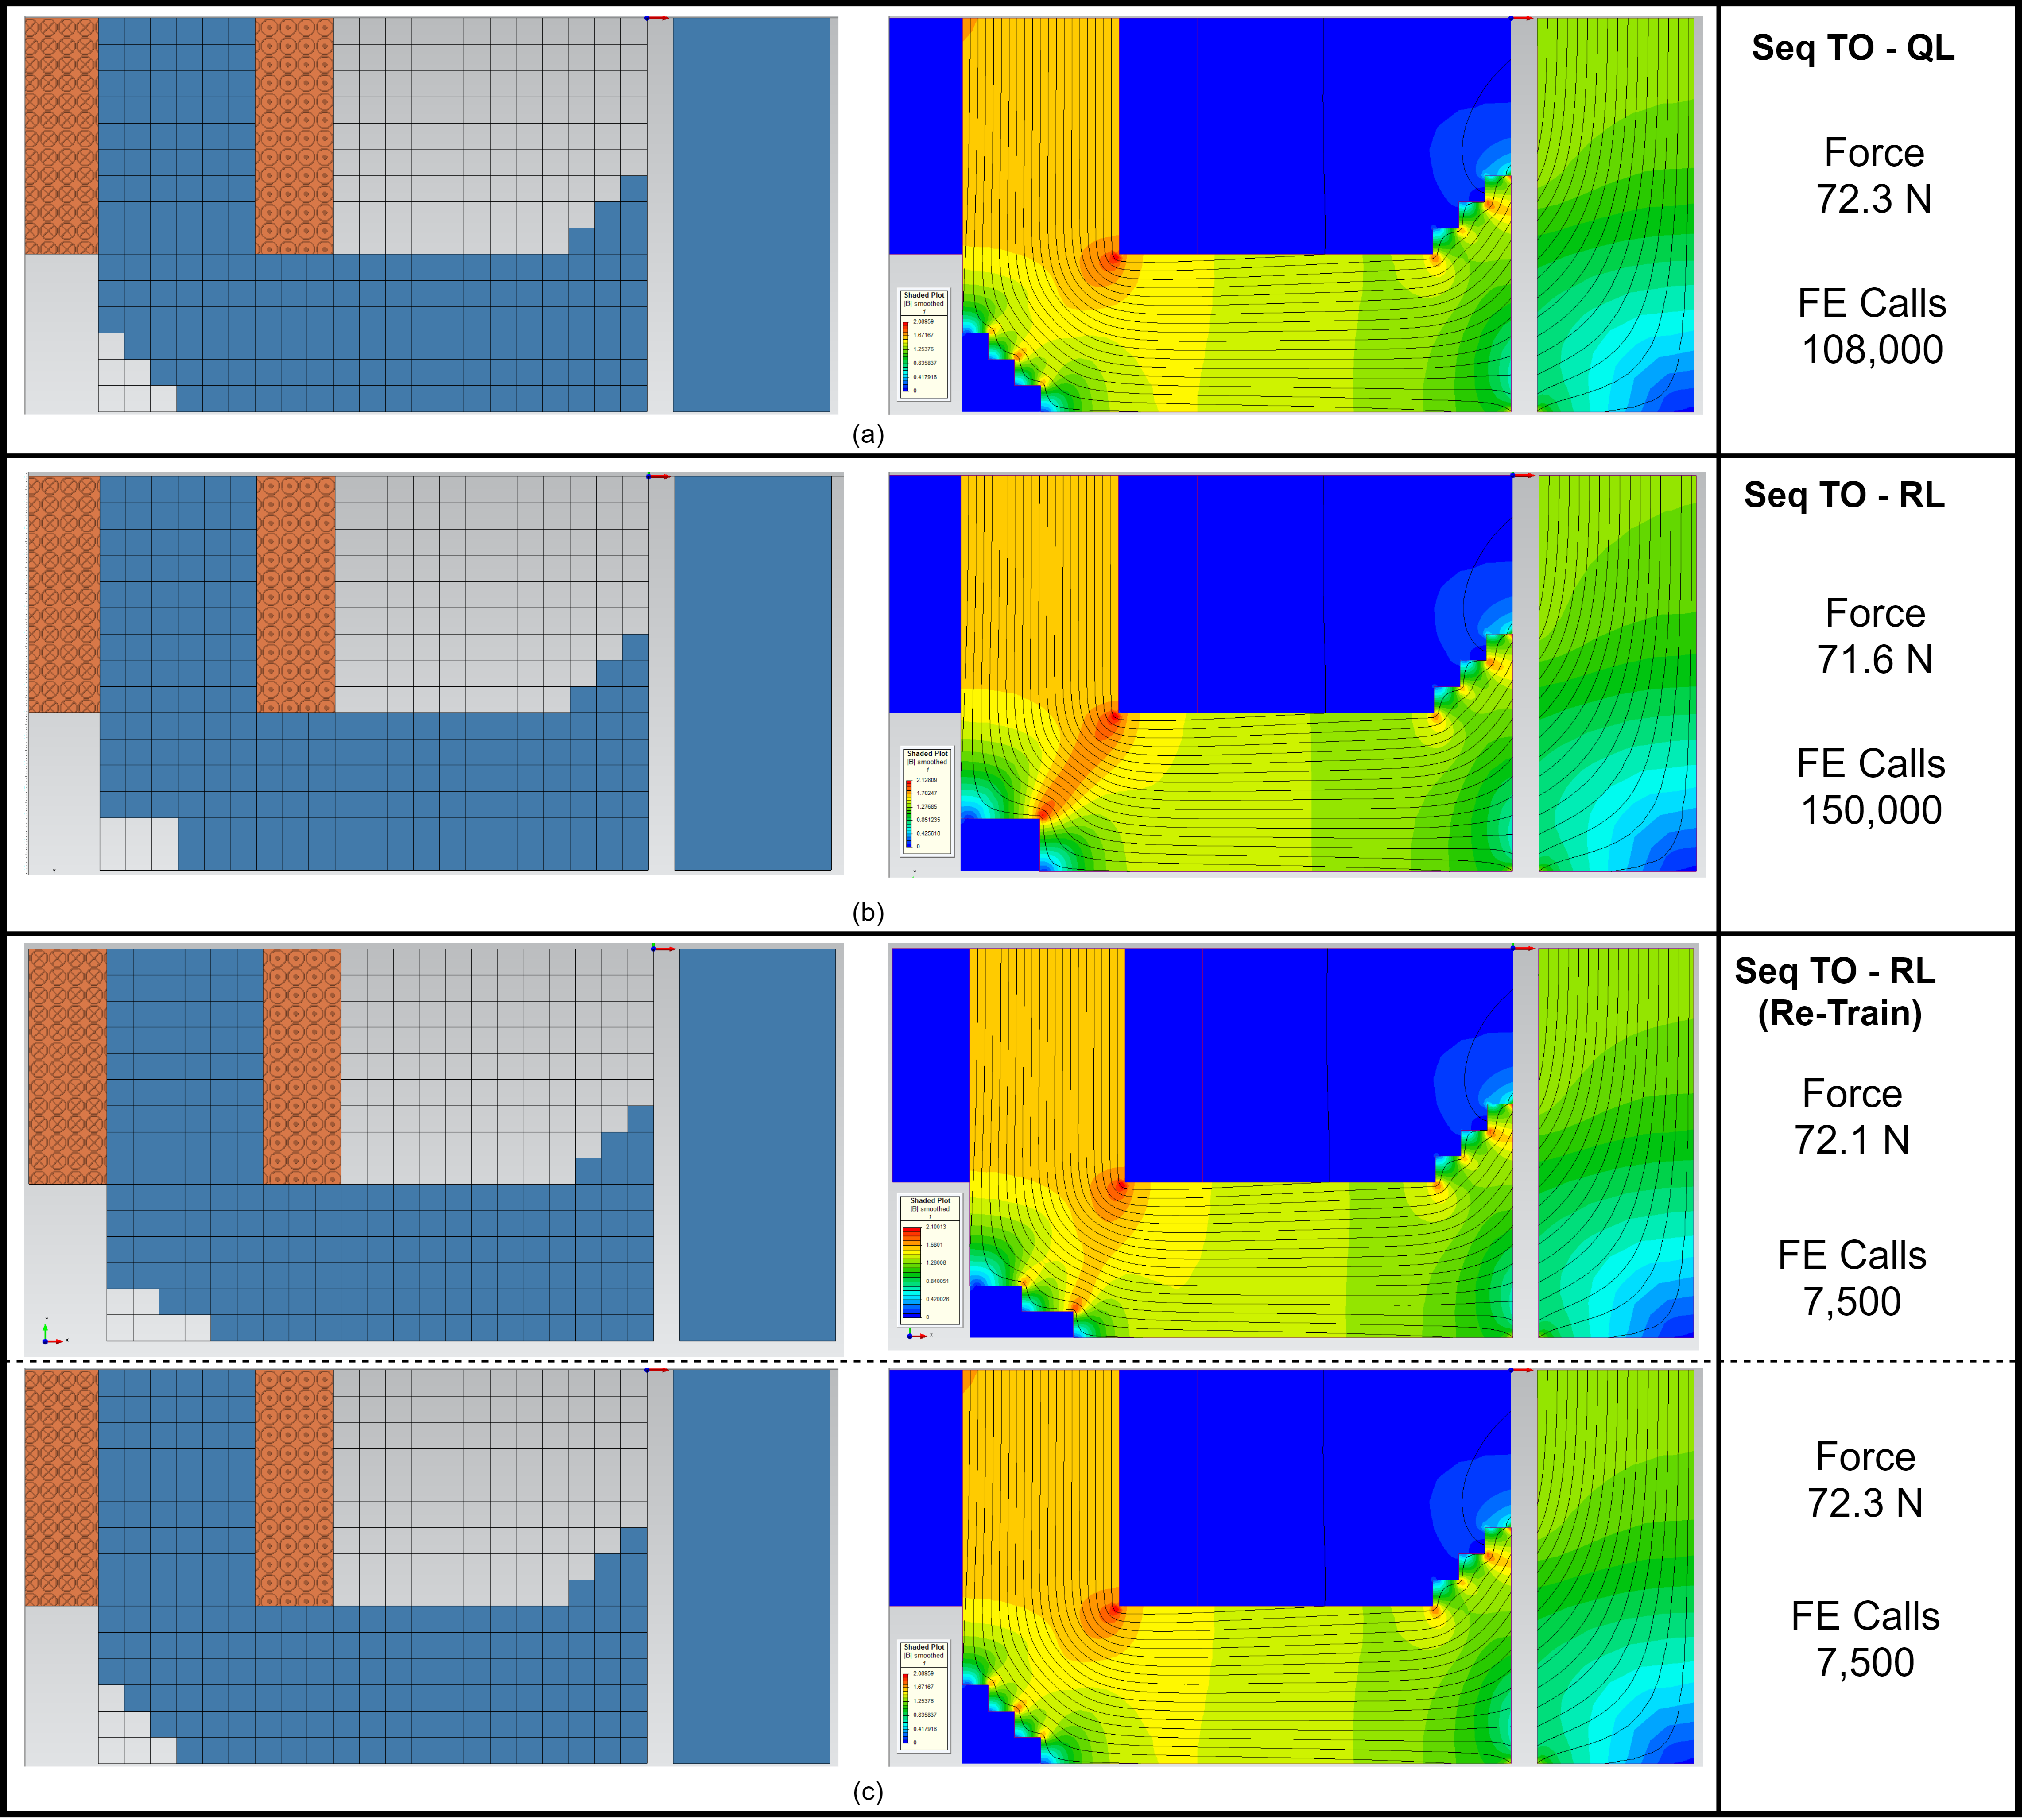
\includegraphics[width=\textwidth]{Figures/Ch_RL/Ccore_1.25A.png}
    \caption{Optimal geometry and B distribution for excitation scenario (1.25 A, 500 Turns) for (a) GA (b) QL based on SeqTO-v1 (c) A2C based on SeqTO-v2.}
    \label{fig:RL_Ccore_1.25A}
\end{figure}

\begin{figure}[h!]
    \centering
    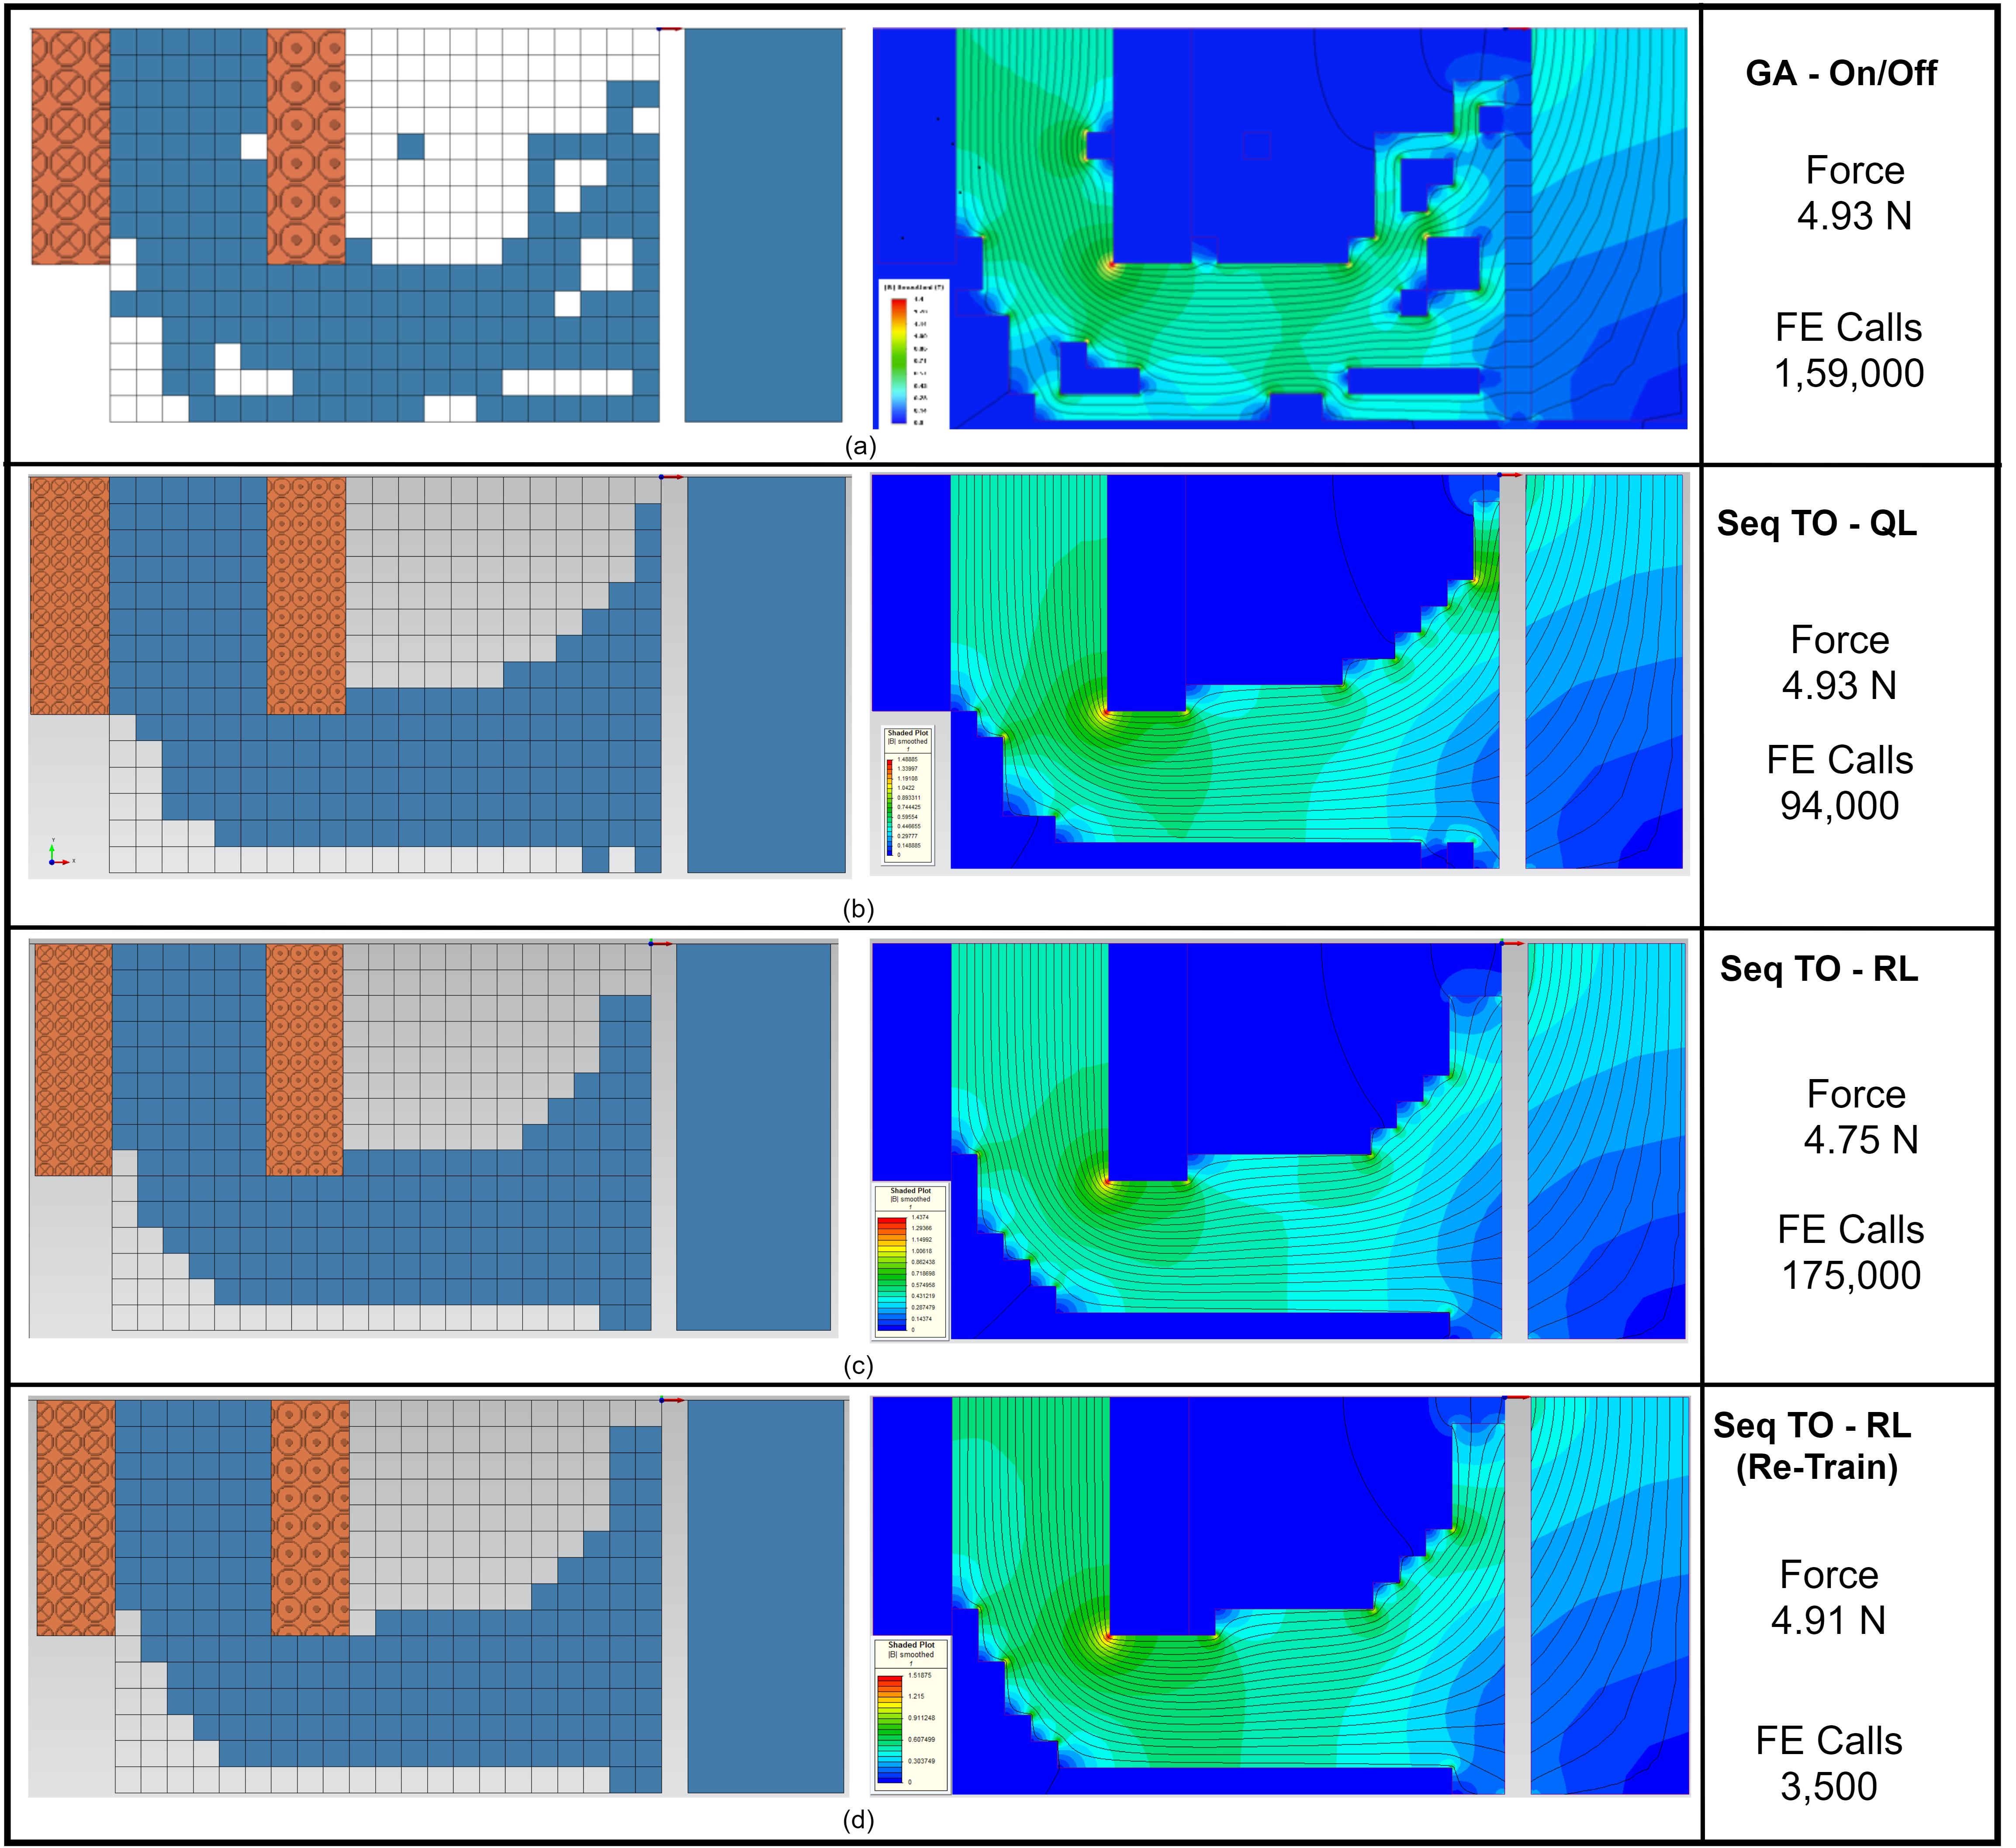
\includegraphics[width=\textwidth]{Figures/Ch_RL/Ccore_0.25A.png}
    \caption{Optimal geometry and B distribution for excitation scenario (0.25 A, 500 Turns) for (a) GA (b) QL based on SeqTO-v1 (c) A2C based on SeqTO-v2.}
    \label{fig:RL_Ccore_0.25A}
\end{figure}


\clearpage
\newpage

The probabilistic nature of A2C (or PG algorithms), as explained in Section \ref{subsec:RL_PG_exploration_n_exploitation} can be seen by two optimal designs obtained for excitation of \textit{1.75 A \& 500 Turns} in Figure \ref{fig:RL_Ccore_1.75A} (b) and for \textit{1.25 A \& 500 Turns} in Figure \ref{fig:RL_Ccore_1.25A}. 
An A2C based agent derives it's action ($a$) from a stochastic policy $\pi_{\theta}(a|s)$, defined as the probability of an agent taking action `$a$' in any state `$s$', and is expressed as 
\begin{align}
    \pi_{\theta}(a|s) = \frac{e^{f(s, a)}}{\sum_{a_i} e^{f(s, a_i)}} \label{eqn:RL_A2C_probabilistic2}
\end{align}
where the policy ($\pi$) has $\theta$ as its parameters and gives a probability distribution for selecting an action `a' over all the possible actions ($a_i$) conditioned on the current state ($s$).
 
This is different for Q-Learning which follows a greedy policy, where the algorithm chooses the same (high valued) action every time. 
\begin{align}
    a^* = \underset{a}{\arg\max} \; Q(s, a)
    \label{eqn:QL_not_probabilistic}
\end{align}

The different nature of deterministic and stochastic policy is the sole reason for multiple optimal geometries obtained for scenarios: \textit{1.25 A \& 500 Turns} and \textit{1.75 A \& 500 Turns}.

\section{Conclusion}

It is verified through numerical optimization that the trained A2C agent acquired a policy to optimize the performance of the C-core actuator while strictly satisfying the volume constraint. Compared with conventional optimization methods such as the evolutionary algorithms, which result in high computational cost for iterative electromagnetic analyses for generating optimal designs, a trained deep learning-based RL method is capable of yielding feasible solutions without any time-consuming iterative analysis process. Although the time required for training is long, the agent once trained requires a significantly lower computational cost compared to GA or Tabular QL for previously unseen excitation conditions, thus showing that the trained agent is generalizable. This capability was demonstrated through different excitation scenarios and the RL agent managed to achieve the optimal solution in most of the training scenarios and close of optimal in the rest. 
These close to optimal topologies (5-10 \% lower performance than optimal) can be further improved upon using re-trainings requiring very little computation cost. Alternatively, these sub-optimal solutions can serve as a starting seed for a different optimization scheme. The inability of the agent to reach the optimal structure can partially be explained due to the inflexibility of the SeqTO-v2 methodology, where the methodology does not support placing a thin strip close to the air gap, as QL can achieve with SeqTO-v1 ($1\ \times 1$). 
However, the number of EM simulations (FE calls) needed to use SeqTO-v1 ($1\ \times 1$) will be simply too much to handle as function approximators, such as neural networks, will require far more training data compared to a deterministic tabular look-up table. An improved version of the SeqTO environment will be explored in the future along with the applicability of other RL algorithms.
Overall, this is a notable display that the agent possesses generalizability over similar topology optimization tasks. 

Although the proposed methodology of Sequence-based TO and sequential decision making using Deep Reinforcement learning algorithms is shown to be capable of providing ``instant" optimal or near-optimal solutions for an electromagnetic device, the proposed TO technique and learning methodology can be easily extended to other fields of designing and engineering where TO is used.


\begin{comment}
\textit{It is verified from the numerical examples that the trained agent acquired a policy to reduce total structural volume while satisfying the stress and displacement constraints. Although it takes a long time for the training, the trained agent requires very low computational cost compared with GA at the application stage. Furthermore, the trained agent is applicable to a truss with different topology, geometry and loading and
boundary conditions after it is trained for a specific truss with various loading and boundary conditions. This applicability was demonstrated through both smaller-scale and larger-scale trusses and sparse sub-optimal topologies were obtained for both cases. 

It is notable that the agent was able to optimize the structure with the unforeseen boundary conditions which the agent has never experienced during the training. It implies that the agent possesses generalized performance for a complex structural optimization task. 
However, in order to create a more reliable agent, it is necessary to implement the training with various topology, geometry, and loading and boundary conditions.Anotherapproachmaybetoincorporatearule-based method to create a hybrid optimization agent. It is also advantageous that the agent is easily replicated and available in other computers by importing the trained parameters. The proposed method for training agent is expected tobecomeasupportingtooltoinstantlyfeedbackthesub-optimal topology and enhance our design exploration.
}

There is not much margin for topological change that could be achieved when the core  near saturation while maintaining the volume constraint.

The test cases are based on an earlier work \parencite{midha_2018} with variation over the excitation (Amp-Turns) from 125 AT to 750 AT. In total, three test cases are selected from \parencite{midha_2018} to test the validity of the proposed algorithm. The previous work is based on a GA and uses different types of filtering \parencite{midha2019selection} to come up with a final optimal solution Table \ref{tab:PG_results}. The results in Table \ref{tab:PG_results} is based on Env. (2) \& (3) with an action dimensionality of eight (Table \ref{tab:env_act_space}) and uses PG based agent. It performs well for all the test cases and improves upon the values obtained from GA with or without filtering. Significantly, for cases with an excitation of 500 AT and 750 AT, the effect of saturation is dominant and the agent can form a policy to tackle the phenomenon of non-linearity.

Furthermore, as can be seen from Figure \ref{fig:750_amp_turn} for an excitation of $750$ AT, that an agent based on Env. (2) and Env. (3) with PG based agent can modify its behaviour based on the response of the environment. This is one single agent able to handle multiple sets of excitation (350, 500, 750 AT) using a single critic, decision element and actor. Thus it can be said that RL based agents mitigate the issue of training an agent afresh for every single test case. 

Results related to optimal geometry and Magnetic flux density distribution for Train Scenario (Coil Current $= 0.5 A$, Coil Turns $= 500$), from different algorithms are shown in Figure \ref{}.

The agent behaviour in the test case of 1 Amp, 500 Turns is shown and discussed in Appendix \ref{appB}.

There is not much margin for topological change that could be achieved when the core  near saturation while maintaining the volume constraint.
The most challenging cases are when the coil excitation is 500 AT and for 750 AT. The optimal agent behaviour are exhibited in Figure \ref{fig:500_amp_turn} and Figure \ref{fig:750_amp_turn} respectively.

The current chapter extends the MDP devised in Chapter \ref{chapter:4_MDP} to account for more complex geometries, while keeping the computational cost low. Having set the MDP, different Reinforcement Learning algorithms were tested such as Q-learning (Tabular \& with function approximators), Policy Gradient algorithm and their extension such as Advantage Actor Critic (A2C), for optimizing the core of a C-core electromagnetic actuator.

\end{comment}